% Customizable fields and text areas start with % >> below.
% Lines starting with the comment character (%) are normally removed before release outside the collaboration, but not those comments ending lines

% svn info. These are modified by svn at checkout time.
% The last version of these macros found before the maketitle will be the one on the front page,
% so only the main file is tracked.
% Do not edit by hand!
\RCS$Revision: 373342 $
\RCS$HeadURL: svn+ssh://svn.cern.ch/reps/tdr2/notes/AN-15-266/trunk/AN-15-266.tex $
\RCS$Id: AN-15-266.tex 373342 2016-11-09 12:27:28Z schoef $
%%%%%%%%%%%%% local definitions %%%%%%%%%%%%%%%%%%%%%
% This allows for switching between one column and two column (cms@external) layouts
% The widths should  be modified for your particular figures. You'll need additional copies if you have more than one standard figure size.
\newlength\cmsFigWidth
\ifthenelse{\boolean{cms@external}}{\setlength\cmsFigWidth{0.85\columnwidth}}{\setlength\cmsFigWidth{0.4\textwidth}}
\ifthenelse{\boolean{cms@external}}{\providecommand{\cmsLeft}{top\xspace}}{\providecommand{\cmsLeft}{left\xspace}}
\ifthenelse{\boolean{cms@external}}{\providecommand{\cmsRight}{bottom\xspace}}{\providecommand{\cmsRight}{right\xspace}}
%%%%%%%%%%%%%%%  Title page %%%%%%%%%%%%%%%%%%%%%%%%
\cmsNoteHeader{AN-15-266} % This is over-written in the CMS environment: useful as preprint no. for export versions
% >> Title: please make sure that the non-TeX equivalent is in PDFTitle below
\title{Search for scalar top quark pair production in the dilepton final state at $\sqrt{s}$ = 13 TeV}



%User defined commands
\newcommand{\todo}[1]{{\bf\color{red}#1}}
\newcommand{\met}{\MET}
\newcommand{\metSig}{S\xspace}
\newcommand{\metSigFull}{\ensuremath{\frac{\met}{\sqrt{H_T}}}\xspace}
\newcommand{\mt}{\ensuremath{M_{T}}\xspace}
\newcommand{\mtll}{\ensuremath{M_{T2}(ll)}\xspace}
\newcommand{\mtbb}{\ensuremath{M_{T2}(bb)}\xspace}
\newcommand{\mtlblb}{\ensuremath{M_{T2}(lblb)}\xspace}
\newcommand{\metPhoton}{\ensuremath{\met(\gamma)}\xspace}
\newcommand{\metSigPhoton}{\ensuremath{S(\gamma)}\xspace}
\newcommand{\Njets}{\ensuremath{n_\text{jet}}\xspace}
\newcommand{\Nbtags}{\ensuremath{n_\text{b-tag}}\xspace}



% >> Authors
%Author is always "The CMS Collaboration" for PAS and papers, so author, etc, below will be ignored in those cases
%For multiple affiliations, create an address entry for the combination
%To mark authors as primary, use the \author* form
%\address[cern]{CERN}
\author[University of Ghent]{Robert Schoefbeck}
\author[University of Ghent]{Didar Dobur}
\author[University of Ghent]{Tom Cornelis}
\author[University of Ghent]{Nicolas Bult\'{e}}
\author[Vrije Universiteit Brussel]{Steven Lowette}
\author[University Of Florida]{Lesya Shchutska}
\author[HEPHY]{Daniel Spitzbart}


% >> Date
% The date is in yyyy/mm/dd format. Today has been
% redefined to match, but if the date needs to be fixed, please write it in this fashion.
% For papers and PAS, \today is taken as the date the head file (this one) was last modified according to svn: see the RCS Id string above.
% For the final version it is best to "touch" the head file to make sure it has the latest date.
\date{\today}

% >> Abstract
% Abstract processing:
% 1. **DO NOT use \include or \input** to include the abstract: our abstract extractor will not search through other files than this one.
% 2. **DO NOT use %**                  to comment out sections of the abstract: the extractor will still grab those lines (and they won't be comments any longer!).
% 3. For PASs: **DO NOT use tex macros**         in the abstract: CDS MathJax processor used on the abstract doesn't understand them _and_ will only look within $$. The abstracts for papers are hand formatted so macros are okay.
\abstract{
   We present a search for direct stop quark production in the opposite-sign dilepton channel using $pp$ collision data at $\sqrt{s}$ = 13 TeV collected by the CMS detector.
   The search is done in both the $ee$, $e\mu$ and $\mu\mu$ channels and involves a base selection of two jets, of which at least one is $b$-tagged, and missing transverse energy.
   The signal regions are defined using "stransverse mass" variables (\mtll, \mtbb, \mtlblb), which efficiently separate the signal from the dominant \ttbar background.
}

% >> PDF Metadata
% Do not comment out the following hypersetup lines (metadata). They will disappear in NODRAFT mode and are needed by CDS.
% Also: make sure that the values of the metadata items are sensible and are in plain text:
% (1) no TeX! -- for \sqrt{s} use sqrt(s) -- this will show with extra quote marks in the draft version but is okay).
% (2) no %.
% (3) No curly braces {}.
\hypersetup{%
pdfauthor={Robert Schoefbeck, Didar Dobur, Tom Cornelis},%
pdftitle={Search for scalar top quark pair production in the dilepton final state at sqrt(s) = 13 TeV},%
pdfsubject={CMS},%
pdfkeywords={CMS, physics, SUSY}}

\maketitle %maketitle comes after all the front information has been supplied
% >> Text
%%%%%%%%%%%%%%%%%%%%%%%%%%%%%%%%  Begin text %%%%%%%%%%%%%%%%%%%%%%%%%%%%%
%% **DO NOT REMOVE THE BIBLIOGRAPHY** which is located before the appendix.
%% You can take the text between here and the bibiliography as an example which you should replace with the actual text of your document.
%% If you include other TeX files, be sure to use "\input{filename}" rather than "\input filename".
%% The latter works for you, but our parser looks for the braces and will break when uploading the document.
%%%%%%%%%%%%%%%

\section{Introduction}

Numerous astronomical observations suggest the existence of a substance that permeates the universe and appears to only interact significantly with ordinary matter via gravity. 
Attempts to directly observe it have been unsuccessful, but this mysterious ``dark matter'' is estimated to make up over a quarter of the total mass-energy in the universe. 
The possibility that dark matter interacts with ordinary matter by other means besides gravitation remains open, implying dark matter may be produced directly by the LHC. 
If produced, dark matter particles are practically invisible to the detector and manifest as missing energy in the event. 
This document describes a search for dark matter produced in association with $\ttbar$ in the dilepton channel with data collected by the CMS detector in 2016 of $\PP$ collisions at $13\:\TeV$.

The simplest and most relevant model for dark matter production with $\ttbar$ proposes a spin-$0$ interaction between dark matter (DM) and Standard Model (SM) particles. 
If the new physics associated with DM satisfies minimal flavour violation, where the couplings between the mediator and the SM particles are Yukawa-type, then heavy flavour (top quark) production is favoured. 
At leading order, the process is gluon-induced and a $\ttbar$ pair is produced with a pair of DM fermions (Fig.~\ref{fig:ttdm_diagram}). 
%The DM fermions can be Dirac or Majorana with the difference being a factor of two in the cross section; they are taken to be Dirac fermions in the signal samples used in this analysis.

\begin{figure}
\centering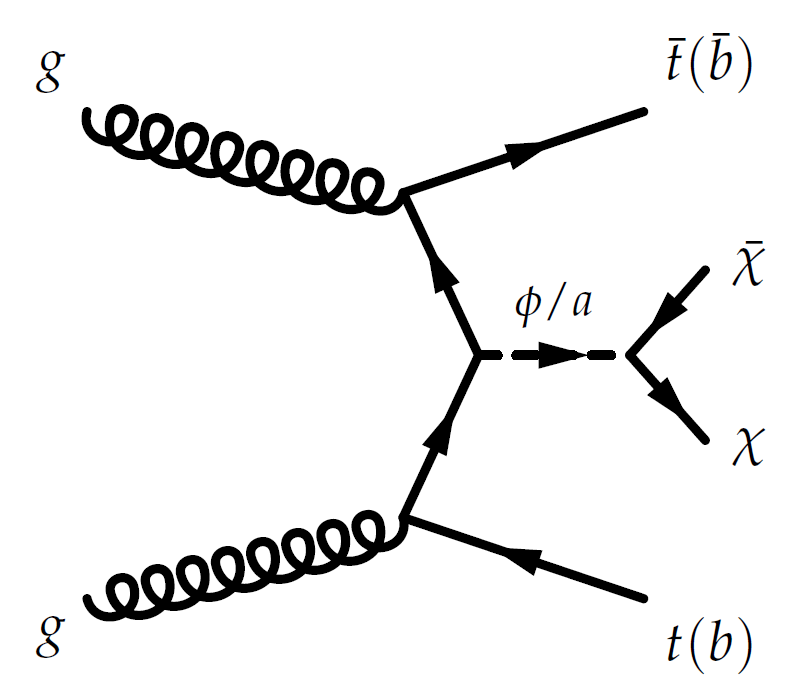
\includegraphics[width=8cm]{figures/ttbarDM.png}
\caption{Leading order diagram in simplified model for $\ttbar+$DM production.}
\label{fig:ttdm_diagram}
\end{figure}

  We use events with two opposite-sign isolated leptons, and two jets with at least one b-tagged jet to perform the search. The stransverse
  mass variable \mtll~\cite{Lester:1999tx} is used to separate the dark matter signal from the Standard Model background, which consists primarily of \ttbar pairs decaying to the dilepton channel.
  The stransverse mass is a generalization of the transverse mass \mt to a system of pair produced particles that decay semi-invisibly. 
  In the case of $W$ boson production, \mt is formed from the transverse momentum of a high \pt lepton (from the $W$ decay) and the missing transverse momentum (\met) in the event, 
  which is assumed to come from the corresponding neutrino. The definition of \mt in the limit where the masses of the daughter particles can be neglected is given by

  \begin{equation}
    \label{eq:mt}
    \mt = \sqrt{2 E_\ell \met \left[1 - \cos(\Delta\phi)\right]}
  \end{equation}

  The transverse mass has the property that if the lepton and the \met both come from the decay of a
  single particle with mass $m$, then $\mt \leq m$. In order to generalize to a system with two particles
  of the same mass, each decaying semi-invisibly, we have to decompose the measured \met into
  a sum of two missing transverse momentum vectors according to %as in Equation~\ref{eq:METsplit}:
 
  \begin{equation}
    \label{eq:METsplit}
    \mathbf{p}_T^{miss} = \mathbf{p}_{T1}^{miss} + \mathbf{p}_{T2}^{miss}.
  \end{equation}

  We may then pair each missing transverse momentum vector with the visible products of the
  decay in order to form \mt for each leg of the pair production. However, since the correct division of the \met into two components is not known, 
  a useful method is to minimize the maximum of the two transverse masses formed under all possible combinations satisfying Equation~\ref{eq:METsplit}. 
  That is, we explore the parameter space of all possible hypothetical neutrino momenta
  that satisfy Equation \ref{eq:METsplit} and for each point in this parameter space we calculate \mt for each half
  of the event and report the maximum of the two. We take the \mtll value for the event to be the
  minimum of the larger \mt value for each such point. This can be represented as %by the expression  for \mtll given in Equation~\ref{eq:mt2ll}:

  \begin{equation}
    \label{eq:mt2ll}
    M_{T2}^2(ll) = \min_{\mathbf{p}_{T1}^{miss} + \mathbf{p}_{T2}^{miss} = \mathbf{p}_T^{miss}} \left( \max \left[ \mt^2(\mathbf{p}_T^{\ell1},\mathbf{p}_{T1}^{miss}) , \mt^2(\mathbf{p}_T^{\ell2},\mathbf{p}_{T2}^{miss}) \right] \right)
  \end{equation}

  It can be shown~\cite{Lester:1999tx} that this definition of \mtll has the same convenient property as the transverse mass: 
  it must be less than the mass of the pair-produced semi-invisibly decaying particle.
  In the case of \ttbar+DM searches in the dilepton channel, the primary challenge comes from separating SM \ttbar 
  production from the signal, since the composition of the final states is identical except
  for invisible particles. In dileptonic \ttbar events the final state is

  \begin{equation*}
    pp \to t + \bar{t} + X \to bW^+ + \bar{b}W^- + X \to b\ell\bar{\nu}_\ell + \bar{b}\bar{\ell}\nu_\ell + X.  
  \end{equation*}

  Assuming that the contribution of the other products $X$ to the \met is not large, the assumptions
  made in the definition of \mtll hold for the lepton-\met system and its value has an upper
  bound at the $W$ mass. On the other hand, dark matter production according to Fig.~\ref{fig:ttdm_diagram}
  provides two extra invisible particles.
  Hence, partitioning of  \met into two components no longer needs to respect an upper bound at the W mass.

  Similarly, one is also able to construct two other variants on the \mtll variable, which take into account the $b$-jets and are expected to have an upper bound at the top mass:

  \begin{align}
    \label{eq:mt2bb}
    M_{T2}^2(bb)   &= \min_{\mathbf{p}_{T1}^{miss} + \mathbf{p}_{T2}^{miss} = \mathbf{p}_T^{miss}} \left( \max_{b \in b_1,b_2} \left[ \mt^2(\mathbf{p}_T^{b},\mathbf{p}_{T1}^{miss}) \right] \right) \\
    M_{T2}^2(lblb) &= \min_{\mathbf{p}_{T1}^{miss} + \mathbf{p}_{T2}^{miss} = \mathbf{p}_T^{miss}} \left( \max_{b \in b_1,b_2, \ell \in \ell_1, \ell_2} \left[ \mt^2(\mathbf{p}_T^{b} + \mathbf{p}_T^{\ell}, \mathbf{p}_{T1}^{miss}) \right] \right)
  \end{align}
  There are two choices how to pair the two leptons  and the two b-jets in the case of \mtlblb. This ambiguity is resolved by minimizing the maximum invariant mass of the two lepton-jet pairs.

  The analysis strategy described in the note uses this property of \mtll, \mtbb and \mtlblb in order to construct
  signal regions, with $\mtll > M_W$, that should have a small
  contamination from dileptonic top decays stemming from the Standard Model.

\section{Samples}

  \subsection{Data samples}

    This analysis uses 2016 pp collision data at $\sqrt{s}$ = 13 TeV, corresponding to an integrated luminosity of 36.4\fbinv. Events are selected from following double-lepton and single-lepton
    primary data sets:

    \begin{itemize}
      \item DoubleEG: two electron channel ($ee$)
      \item DoubleMuon: two muon channel ($\mu\mu$)
      \item MuonEG: one electron and one muon channel ($e\mu$)
      \item SingleElectron: backup for $ee$ and $e\mu$ channels
      \item SingleMuon: backup for $\mu\mu$ and $e\mu$ channels
    \end{itemize}

    For each of the primary data sets, runs 2016B to 2016H are considered:
    \begin{itemize}
      \item {\verb /<PD>/Run2016B-23Sep2016-v3/MINIAOD } (run 272007-275376)
      \item {\verb /<PD>/Run2016C-23Sep2016-v1/MINIAOD } (run 275657-276283)
      \item {\verb /<PD>/Run2016D-23Sep2016-v1/MINIAOD } (run 276315-276811)
      \item {\verb /<PD>/Run2016E-23Sep2016-v1/MINIAOD } (run 276831-277420)
      \item {\verb /<PD>/Run2016F-23Sep2016-v1/MINIAOD } (run 277772-278808)
      \item {\verb /<PD>/Run2016G-23Sep2016-v1/MINIAOD } (run 278820-280385)
      \item {\verb /<PD>/Run2016H-PromptReco-v2/MINIAOD } (run 280919-284035)
      \item {\verb /<PD>/Run2016H-PromptReco-v3/MINIAOD } (run 284036-284068)
    \end{itemize}
    and processed using the {\verb Cert_271036-284044_13TeV_23Sep2016ReReco_Collisions16_JSON } golden JSON file where all CMS subdetectors are flagged as good.


  \subsection{Simulation}
    Background samples have been produced in the Spring16 miniAODv2 campaign and have an average pile-up of $\mu = 20$ and a bunch crossing spacing of 25ns.
    The backgrounds are listed in Table \ref{samples-backgrounds2016} along with their theoretical cross sections.
    \begin{table}
  \center
  \tiny
  \begin{tabular}{l|l|l}
     process                & dataset path & $\sigma \cdot BR$ (pb)\\
     \hline
     Drell-Yan              & \verb /DYJetsToLL_M-5to50_TuneCUETP8M1_13TeV-madgraphMLM-pythia8/[Spring16mAOD]-v1/MINIAODSIM \; (for $H_T < 100$ GeV)          & 71310 \\ 
                            & \verb /DYJetsToLL_M5to50_HT-100to200_TuneCUETP8M1_13TeV-madgraphMLM-pythia8/[Spring16mAOD]-v1/MINIAODSIM                        & 224.2 \\
                            & \verb /DYJetsToLL_M5to50_HT-100to200_TuneCUETP8M1_13TeV-madgraphMLM-pythia8/[Spring16mAOD]_etx1-v1/MINIAODSIM                   & 224.2 \\
                            & \verb /DYJetsToLL_M5to50_HT-200to400_TuneCUETP8M1_13TeV-madgraphMLM-pythia8/[Spring16mAOD]-v1/MINIAODSIM                        & 37.2 \\
                            & \verb /DYJetsToLL_M5to50_HT-200to400_TuneCUETP8M1_13TeV-madgraphMLM-pythia8/[Spring16mAOD]_ext1-v1/MINIAODSIM                   & 37.2 \\
                            & \verb /DYJetsToLL_M5to50_HT-400to600_TuneCUETP8M1_13TeV-madgraphMLM-pythia8/[Spring16mAOD]-v1/MINIAODSIM                        & 3.581 \\
                            & \verb /DYJetsToLL_M5to50_HT-600toInf_TuneCUETP8M1_13TeV-madgraphMLM-pythia8/[Spring16mAOD]-v1/MINIAODSIM                        & 1.124 \\
                            & \verb /DYJetsToLL_M5to50_HT-600toInf_TuneCUETP8M1_13TeV-madgraphMLM-pythia8/[Spring16mAOD]_ext1-v1/MINIAODSIM                   & 1.124 \\
                            & \verb /DYJetsToLL_M-50_TuneCUETP8M1_13TeV-madgraphMLM-pythia8/[Spring16mAOD]_ext1-v1/MINIAODSIM \; (for $H_T < 100$ GeV)        & 5765.4 \\
                            & \verb /DYJetsToLL_M-50_HT-100to200_TuneCUETP8M1_13TeV-madgraphMLM-pythia8/[Spring16mAOD]-v1/MINIAODSIM                          & 171.5 \\
                            & \verb /DYJetsToLL_M-50_HT-100to200_TuneCUETP8M1_13TeV-madgraphMLM-pythia8/[Spring16mAOD]_ext1-v1/MINIAODSIM                     & 171.5 \\
                            & \verb /DYJetsToLL_M-50_HT-200to400_TuneCUETP8M1_13TeV-madgraphMLM-pythia8/[Spring16mAOD]-v1/MINIAODSIM                          & 52.58 \\
                            & \verb /DYJetsToLL_M-50_HT-200to400_TuneCUETP8M1_13TeV-madgraphMLM-pythia8/[Spring16mAOD]_ext1-v1/MINIAODSIM                     & 52.58 \\
                            & \verb /DYJetsToLL_M-50_HT-400to600_TuneCUETP8M1_13TeV-madgraphMLM-pythia8/[Spring16mAOD]-v1/MINIAODSIM                          & 6.761 \\
                            & \verb /DYJetsToLL_M-50_HT-400to600_TuneCUETP8M1_13TeV-madgraphMLM-pythia8/[Spring16mAOD]_ext1-v1/MINIAODSIM                     & 6.761 \\
                            & \verb /DYJetsToLL_M-50_HT-600toInf_TuneCUETP8M1_13TeV-madgraphMLM-pythia8/[Spring16mAOD]-v1/MINIAODSIM                          & 2.72 \\
                            & \verb /DYJetsToLL_M-50_HT-600toInf_TuneCUETP8M1_13TeV-madgraphMLM-pythia8/[Spring16mAOD]_ext1-v1/MINIAODSIM                     & 2.72 \\
     $t\bar{t}$       %      & \verb /TTTo2L2Nu_13TeV-powheg/[Spring16mAOD]-v1/MINIAODSIM                                                                      & 87.31 \\
                            & \verb /TTTo2L2Nu_13TeV-powheg/[Spring16mAOD*]_ext3-v1/MINIAODSIM						                      & 87.31 \\
     single $t$             & \verb /ST_tW_top_5f_inclusiveDecays_13TeV-powheg-pythia8_TuneCUETP8M1/[Spring16mAOD]-v2/MINIAODSIM			      & 35.6 \\
                            & \verb /ST_tW_antitop_5f_inclusiveDecays_13TeV-powheg-pythia8_TuneCUETP8M1/[Spring16mAOD]-v1/MINIAODSIM                          & 35.6 \\
                      %      & \verb /ST_t-channel_4f_leptonDecays_13TeV-amcatnlo-pythia8_TuneCUETP8M1/[Spring16mAOD]-v1/MINIAODSIM                            & 70.31 \\
                      %      & \verb /ST_t-channel_4f_leptonDecays_13TeV-amcatnlo-pythia8_TuneCUETP8M1/[Spring16mAOD]_ext1-v1/MINIAODSIM                       & 70.31 \\
     $t\bar{t}Z$      %      & \verb /TTZToQQ_TuneCUETP8M1_13TeV-amcatnlo-pythia8/[Spring16mAOD]-v1/MINIAODSIM                                                 & 0.5297 \\
                      %      & \verb /TTZToLLNuNu_M-10_TuneCUETP8M1_13TeV-amcatnlo-pythia8/[Spring16mAOD]-v1/MINIAODSIM                                        & 0.2529 \\
                            & \verb /ttZJets_13TeV_madgraphMLM/[Spring16mAOD]]-v1/MINIAODSIM                                                                  & 0.7826 \\
     $t\bar{t}W$            & \verb /TTWJetsToLNu_TuneCUETP8M1_13TeV-amcatnloFXFX-madspin-pythia8/[Spring16mAOD]-v1/MINIAODSIM                                & 0.2043 \\
                            & \verb /TTWJetsToQQ_TuneCUETP8M1_13TeV-amcatnloFXFX-madspin-pythia8/[Spring16mAOD]-v1/MINIAODSIM                                 & 0.4062 \\
     $t\bar{t}H$            & \verb /ttHJetToNonbb_M125_13TeV_amcatnloFXFX_madspin_pythia8_mWCutfix/[Spring16mAOD*]_ext1-v2\MINIAODSIM                        & 0.2151 \\
     $tZq$                  & \verb /tZq_ll_4f_13TeV-amcatnlo-pythia8_TuneCUETP8M1/[Spring16mAOD]-v1/MINIAODSIM                                               & 0.0758 \\
                     %       & \verb /tZq_nunu_4f_13TeV-amcatnlo-pythia8_TuneCUETP8M1/[Spring16mAOD]-v1/MINIAODSIM 					    & 0.1379 \\
%    $t\bar{t}\gamma$       & \verb /TTGJets_TuneCUETP8M1_13TeV-amcatnloFXFX-madspin-pythia8/[Spring16mAOD]-v1/MINIAODSIM                                     & 3.697 \\
     $WW, WZ, ZZ$           & \verb /WWTo1L1Nu2Q_13TeV_amcatnloFXFX_madspin_pythia8/[Spring16mAOD]-v1/MINIAODSIM                                              & 49.997 \\
                            & \verb /WWToLNuQQ_13TeV-powheg/[Spring16mAOD]-v1/MINIAODSIM                                                                      & 43.53 \\
                            & \verb /WWToLNuQQ_13TeV-powheg/[Spring16mAOD]_ext1-v1/MINIAODSIM                                                                 & 43.53 \\
                            & \verb /WZTo1L3Nu_13TeV_amcatnloFXFX_madspin_pythia8/[Spring16mAOD]-v1/MINIAODSIM                                                & 3.054 \\
                            & \verb /WZTo1L1Nu2Q_13TeV_amcatnloFXFX_madspin_pythia8/[Spring16mAOD]-v1/MINIAODSIM                                              & 10.71 \\
                            & \verb /WZTo2L2Q_13TeV_amcatnloFXFX_madspin_pythia8/[Spring16mAOD]-v1/MINIAODSIM                                                 & 5.60 \\
                            & \verb /WZTo3LNu_TuneCUETP8M1_13TeV-powheg-pythia8/[Spring16mAOD]-v1/MINIAODSIM                                                  & 4.42965 \\
                            & \verb /ZZTo2L2Q_13TeV_amcatnloFXFX_madspin_pythia8/[Spring16mAOD]-v1/MINIAODSIM                                                 & 3.28 \\
                            & \verb /ZZTo2Q2Nu_13TeV_amcatnloFXFX_madspin_pythia8/[Spring16mAOD]-v1/MINIAODSIM                                                & 4.04 \\
                            & \verb /VVTo2L2Nu_13TeV_amcatnloFXFX_madspin_pythia8/[Spring16mAOD]-v1/MINIAODSIM                                                & 11.95 \\
     tribosons              & \verb /WWW_4F_TuneCUETP8M1_13TeV-amcatnlo-pythia8/[Spring16mAOD]-v1/MINIAODSIM                                                  & 0.2086 \\
                            & \verb /WWZ_TuneCUETP8M1_13TeV-amcatnlo-pythia8/[Spring16mAOD]-v1/MINIAODSIM                                                     & 0.1651 \\
                            & \verb /WZZ_TuneCUETP8M1_13TeV-amcatnlo-pythia8/[Spring16mAOD]-v1/MINIAODSIM                                                     & 0.05565 \\
                            & \verb /ZZZ_TuneCUETP8M1_13TeV-amcatnlo-pythia8/[Spring16mAOD]-v1/MINIAODSIM                                                     & 0.01398 \\
  \end{tabular}\\
  \vspace{2mm}
    \verb [Spring16mAOD] = \verb RunIISpring16MiniAODv2-PUSpring16_80X_mcRun2_asymptotic_2016_miniAODv2_v0 \\
    \verb [Spring16mAOD*] = \verb RunIISpring16MiniAODv2-PUSpring16RAWAODSIM_80X_mcRun2_asymptotic_2016_miniAODv2_v0 \\
  \caption{Background samples}
  \label{samples-backgrounds2016}
\end{table}

    Signal samples are listed in Table \ref{samples-signals2016}.
    \begin{table}
  \center
  \tiny
  \begin{tabular}{l|l}
     process                & dataset \\ 
     \hline
     T2tt signal            & \verb /SMS-T2tt_mStop-150to250_TuneCUETP8M1_13TeV-madgraphMLM-pythia8/[Spring16mAODFS]-v1/MINIAODSIM \\
                            & \verb /SMS-T2tt_mStop-250to350_TuneCUETP8M1_13TeV-madgraphMLM-pythia8/[Spring16mAODFS]-v1/MINIAODSIM \\ 
                            & \verb /SMS-T2tt_mStop-350to400_TuneCUETP8M1_13TeV-madgraphMLM-pythia8/[Spring16mAODFS]-v1/MINIAODSIM \\ 
                            & \verb /SMS-T2tt_mStop-400to1200_TuneCUETP8M1_13TeV-madgraphMLM-pythia8/[Spring16mAODFS]-v1/MINIAODSIM \\
                            & \verb /SMS-T2tt_mStop-425_mLSP-325_TuneCUETP8M1_13TeV-madgraphMLM-pythia8/[Spring16mAODFS]-v1/MINIAODSIM \\
                            & \verb /SMS-T2tt_mStop-500_mLSP-325_TuneCUETP8M1_13TeV-madgraphMLM-pythia8/[Spring16mAODFS]-v2/MINIAODSIM \\
                            & \verb /SMS-T2tt_mStop-850_mLSP-100_TuneCUETP8M1_13TeV-madgraphMLM-pythia8/[Spring16mAODFS]-v1/MINIAODSIM \\
  \end{tabular}\\
  \vspace{2mm}
     \verb [Spring16mAODFS] = \verb RunIISpring16MiniAODv2-PUSpring16Fast_80X_mcRun2_asymptotic_2016_miniAODv2_v0 \\
  \caption{FastSim Signal samples scanning $m_{\sTop}$ between 150 and 1200 GeV.}
  \label{samples-signals2016}
\end{table}


\section{Triggers}
\label{sec:trigger}

In this analysis we use various sets of triggers in order to achieve an optimal selection efficiency. For each dilepton channel ($ee$, $\mu\mu$ and $e\mu$) we take the logical OR
of the dilepton triggers listed in Tab.~\ref{table:triggers} thus combining isolated and non-isolated triggers.
We moreover complement the partially inefficient dilepton triggers by single lepton triggers and remove the overlap between two primary data sets by vetoing events that 
fired a dilepton trigger in the single lepton primary data sets.
Because the e$\mu$ channel is complemented by two single lepton primary data sets, the procedure has two steps: We first add events from the {\verb SingleElectron } primary data set
that fired single electron triggers but failed the double lepton triggers that we use to select events in the {\verb MuonEG } primary data set. We furthermore add events from the
{\verb SingleMuon } primary data set that fired single muon triggers but fired none of the triggers we use to select events in either the {\verb MuonEG } or the {\verb SingleElectron } primary data set.

Table \ref{table:triggers} gives an overview of all triggers used in this analysis.

\begin{table}
  \center
  \scriptsize
  \begin{tabular}{c|l|l}
     channel  & primary dataset & HLT paths\\
     \hline
     $ee$     & DoubleEG        & \verb HLT_Ele23_Ele12_CaloIdL_TrackIdL_IsoVL_DZ \\
              &                 & \verb HLT_Ele17_Ele12_CaloIdL_TrackIdL_IsoVL_DZ \\
              &                 & \verb HLT_DoubleEle33_CaloIdL_GsfTrkIdVL \\
              &                 & \verb HLT_DoubleEle33_CaloIdL_GsfTrkIdVL_MW \\
              & SingleElectron  & \verb HLT_Ele105_CaloIdVT_GsfTrkIdT \\
              &                 & \verb HLT_Ele115_CaloIdVT_GsfTrkIdT \\
     \hline
     $\mu\mu$ & DoubleMuon      & \verb HLT_Mu17_TrkIsoVVL_Mu8_TrkIsoVVL \\
              &                 & \verb HLT_Mu17_TrkIsoVVL_Mu8_TrkIsoVVL_DZ \\
              &                 & \verb HLT_Mu17_TrkIsoVVL_TkMu8_TrkIsoVVL \\
              &                 & \verb HLT_Mu17_TrkIsoVVL_TkMu8_TrkIsoVVL_DZ \\
              &                 & \verb HLT_Mu30_TkMu11 \\
              & SingleMuon      & \verb HLT_Mu50 \\
              &                 & \verb HLT_TkMu50 \\
              &                 & \verb HLT_Mu45_eta2p1 \\
     \hline
     $e\mu$   & MuonEG          & \verb HLT_Mu23_TrkIsoVVL_Ele12_CaloIdL_TrackIdL_IsoVL \\
              &                 & \verb HLT_Mu17_TrkIsoVVL_Ele12_CaloIdL_TrackIdL_IsoVL \\
              &                 & \verb HLT_Mu8_TrkIsoVVL_Ele23_CaloIdL_TrackIdL_IsoVL \\
              &                 & \verb HLT_Mu8_TrkIsoVVL_Ele17_CaloIdL_TrackIdL_IsoVL \\
              &                 & \verb HLT_Mu30_Ele30_CaloIdL_GsfTrkIdVL \\
              & SingleElectron  & \verb HLT_Ele105_CaloIdVT_GsfTrkIdT \\
              &                 & \verb HLT_Ele115_CaloIdVT_GsfTrkIdT \\
              & SingleMuon      & \verb HLT_Mu50 \\
              &                 & \verb HLT_TkMu50 \\
              &                 & \verb HLT_Mu45_eta2p1 \\
  \end{tabular}
  \caption{Summary of HLT triggers grouped by channel and primary dataset. }
  \label{table:triggers}
\end{table}

%\subsection{Trigger efficiencies}

% figures from http://schoef.web.cern.ch/schoef/pngEff/
\begin{figure}
  \centering
  %\subfloat[only isolated double-lepton triggers][only isolated \\ double-lepton triggers]{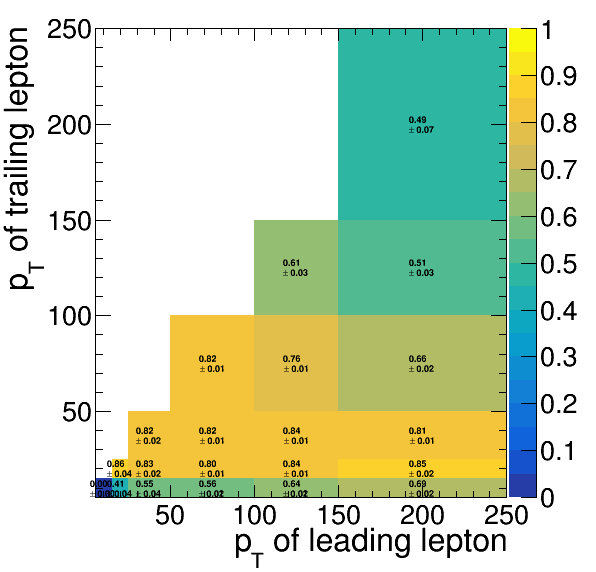
\includegraphics[width=0.5\textwidth]{figures/trigger/HLT_mumu_pt1_pt2_highEta1_NOAddTrig.png}}
  %\subfloat[including non-isolated double-lepton triggers][including non-isolated \\ double-lepton triggers]{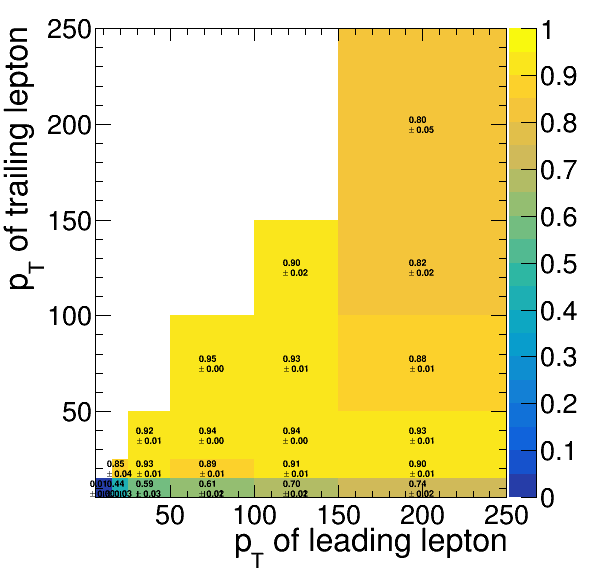
\includegraphics[width=0.5\textwidth]{figures/trigger/HLT_mumu_pt1_pt2_highEta1_DoubleLepTrigOR.png}}\\
  %\subfloat[including single-lepton triggers][including \\ single-lepton triggers]{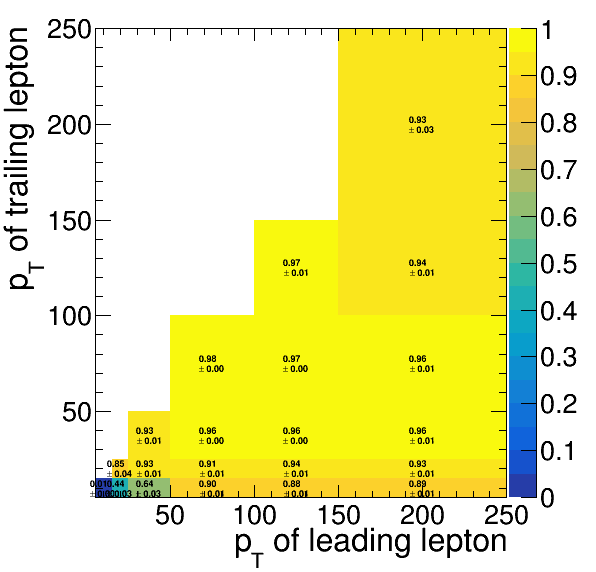
\includegraphics[width=0.5\textwidth]{figures/trigger/HLT_mumu_pt1_pt2_highEta1_AllTriggersInOR.png}}
  \subfloat[only isolated double-lepton triggers][only isolated \\ double-lepton triggers]{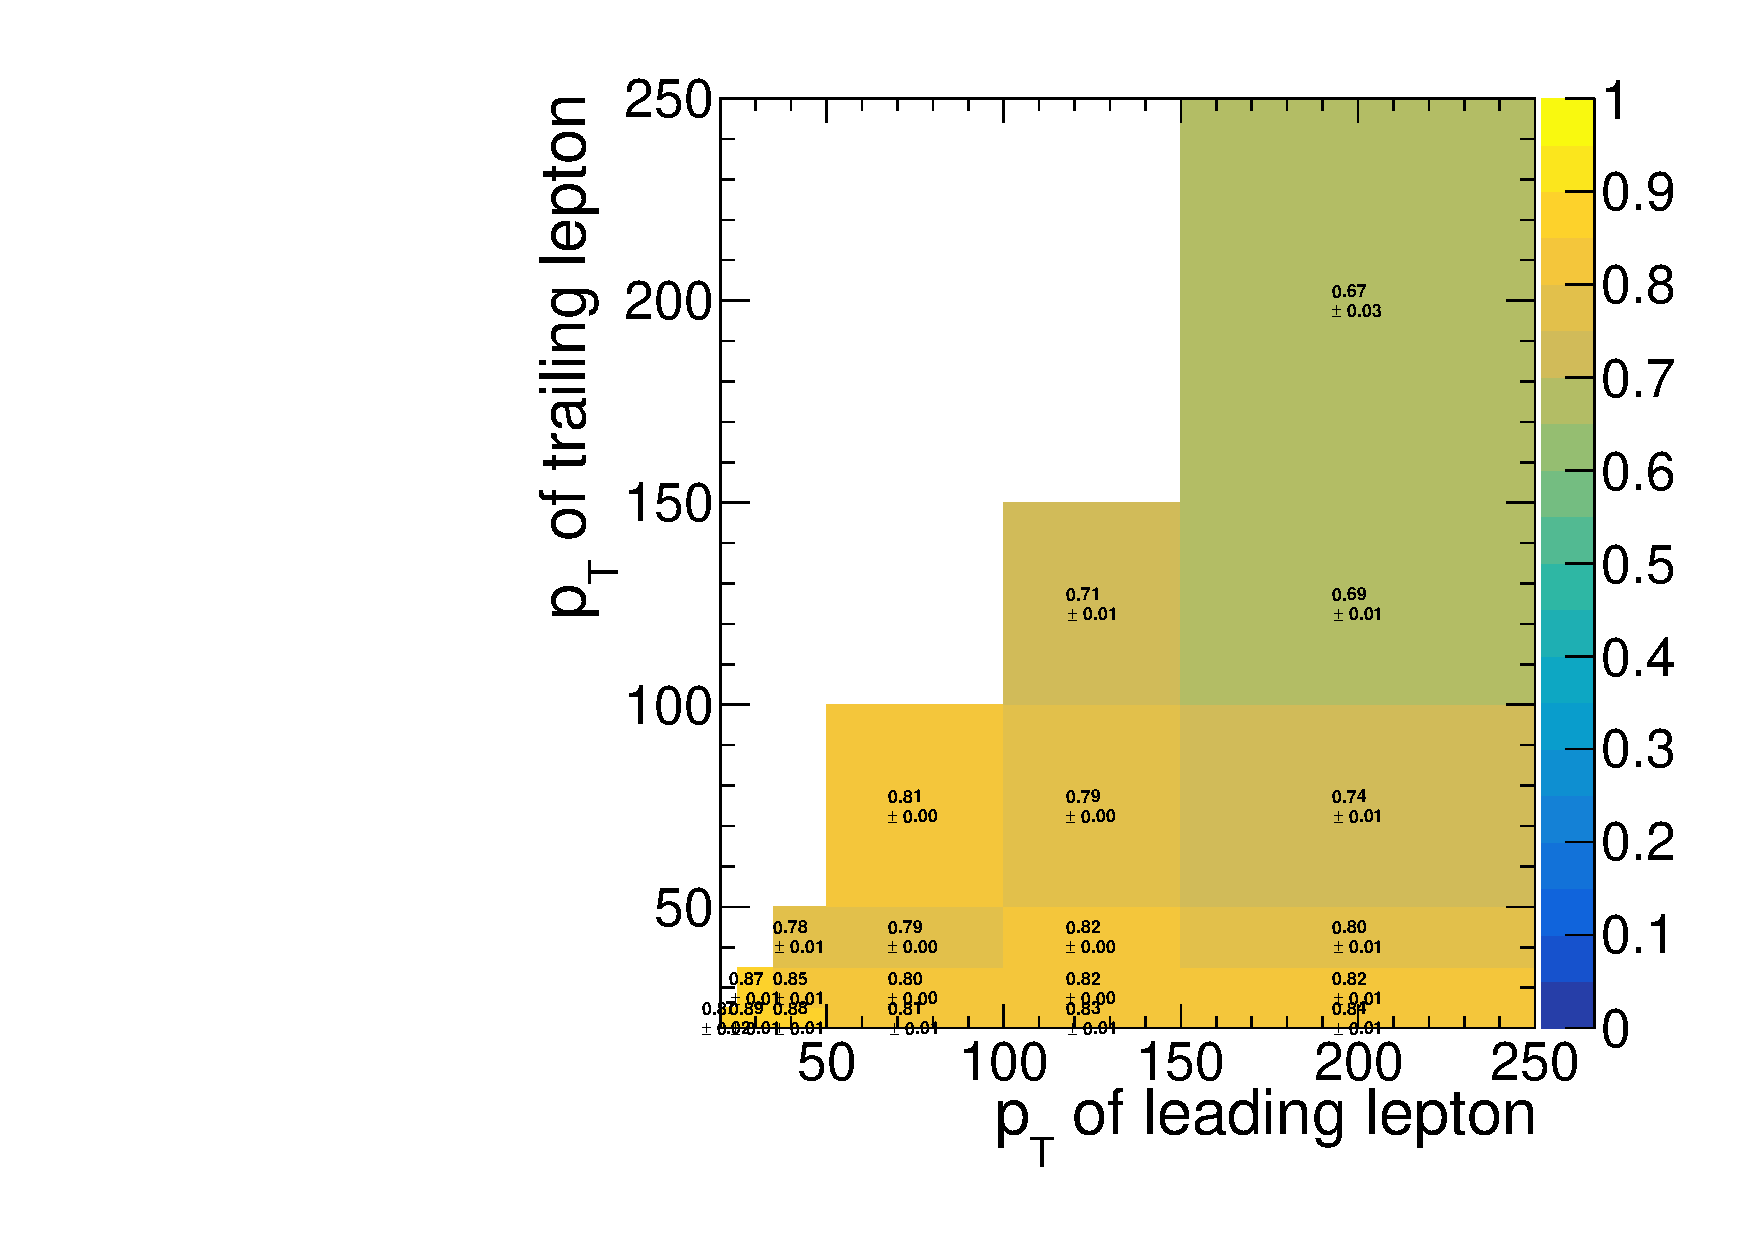
\includegraphics[width=0.5\textwidth]{figures/trigger/HLT_mumuIso_pt1_pt2_highEta1_veryCoarse_BCDEF.pdf}}
  \subfloat[including non-isolated double-lepton triggers][including non-isolated \\ double-lepton triggers]{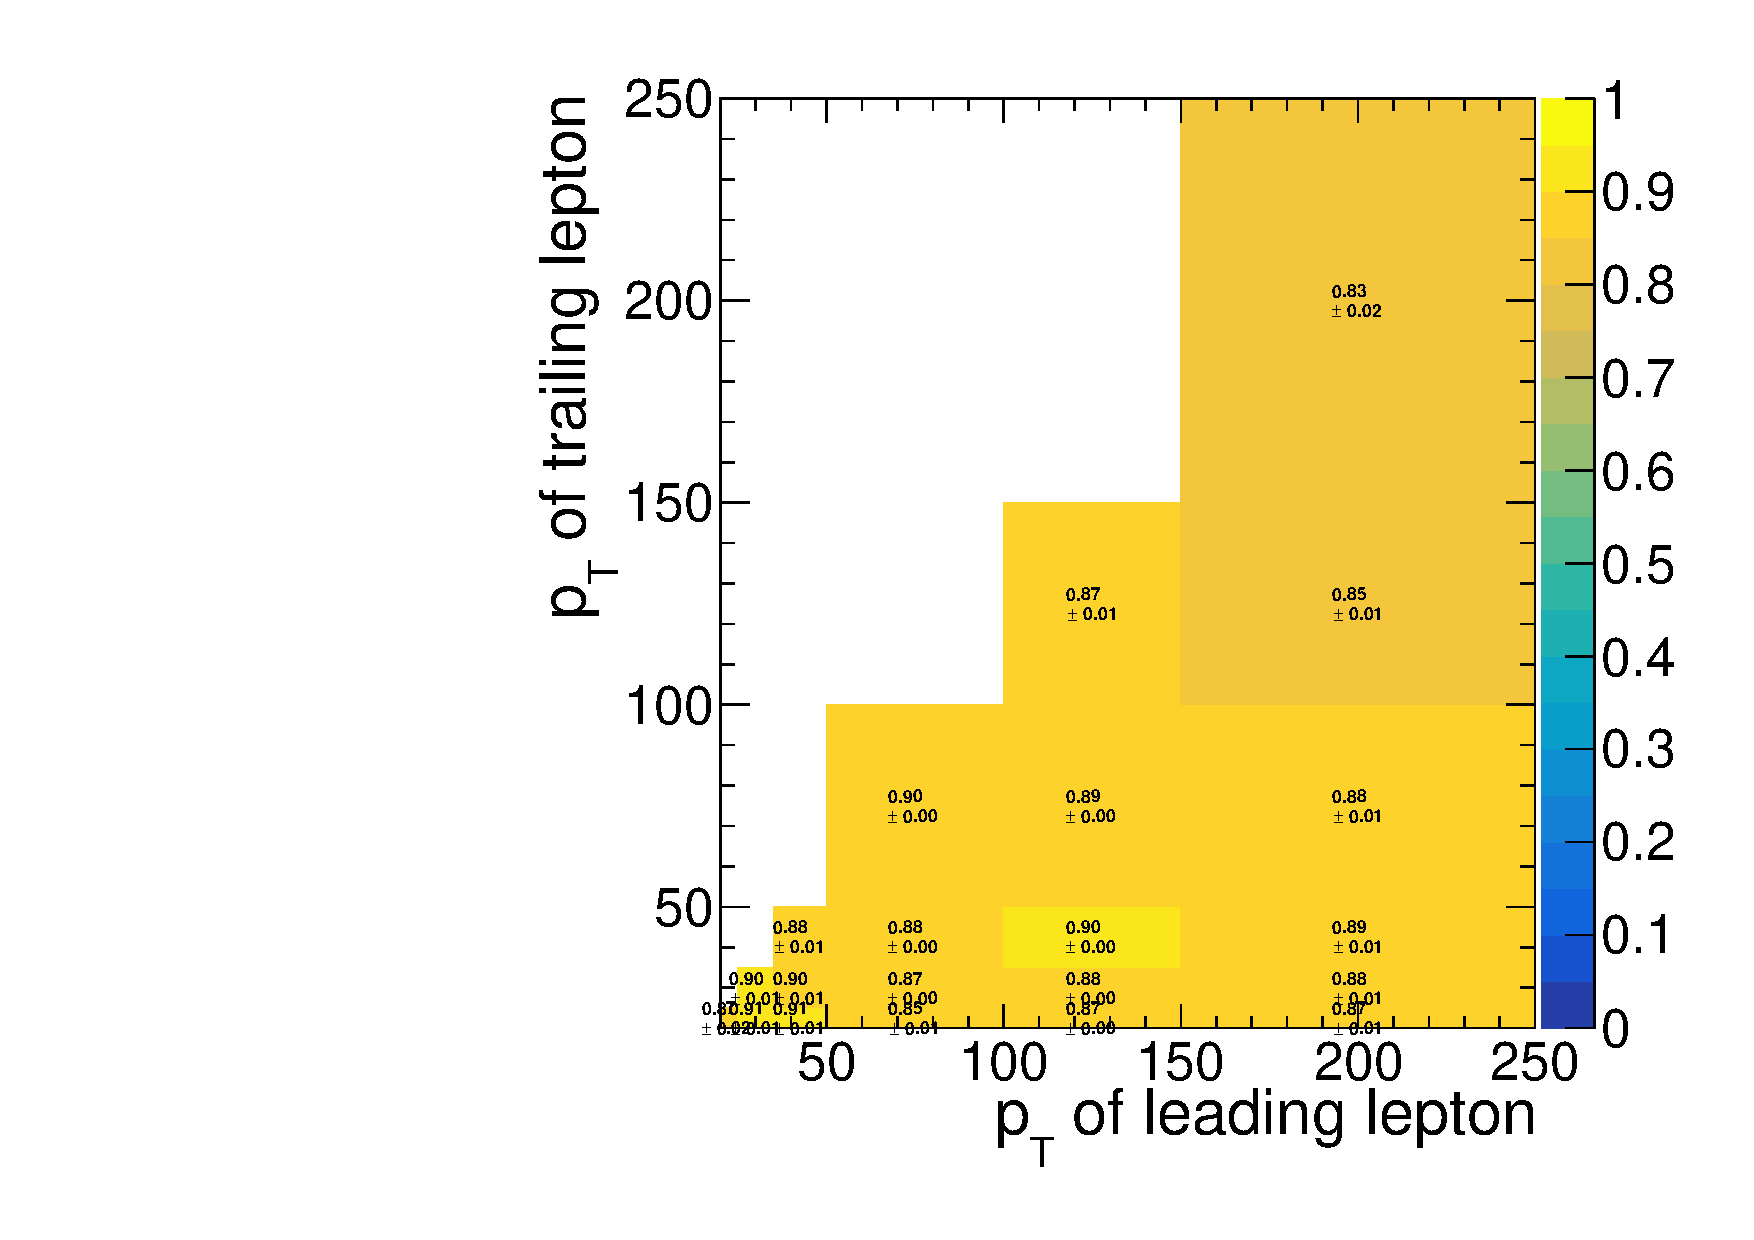
\includegraphics[width=0.5\textwidth]{figures/trigger/HLT_mumuIso_OR_HLT_mumuNoiso_pt1_pt2_highEta1_veryCoarse_BCDEF.pdf}}\\
  \subfloat[including single-lepton triggers][including \\ single-lepton triggers]{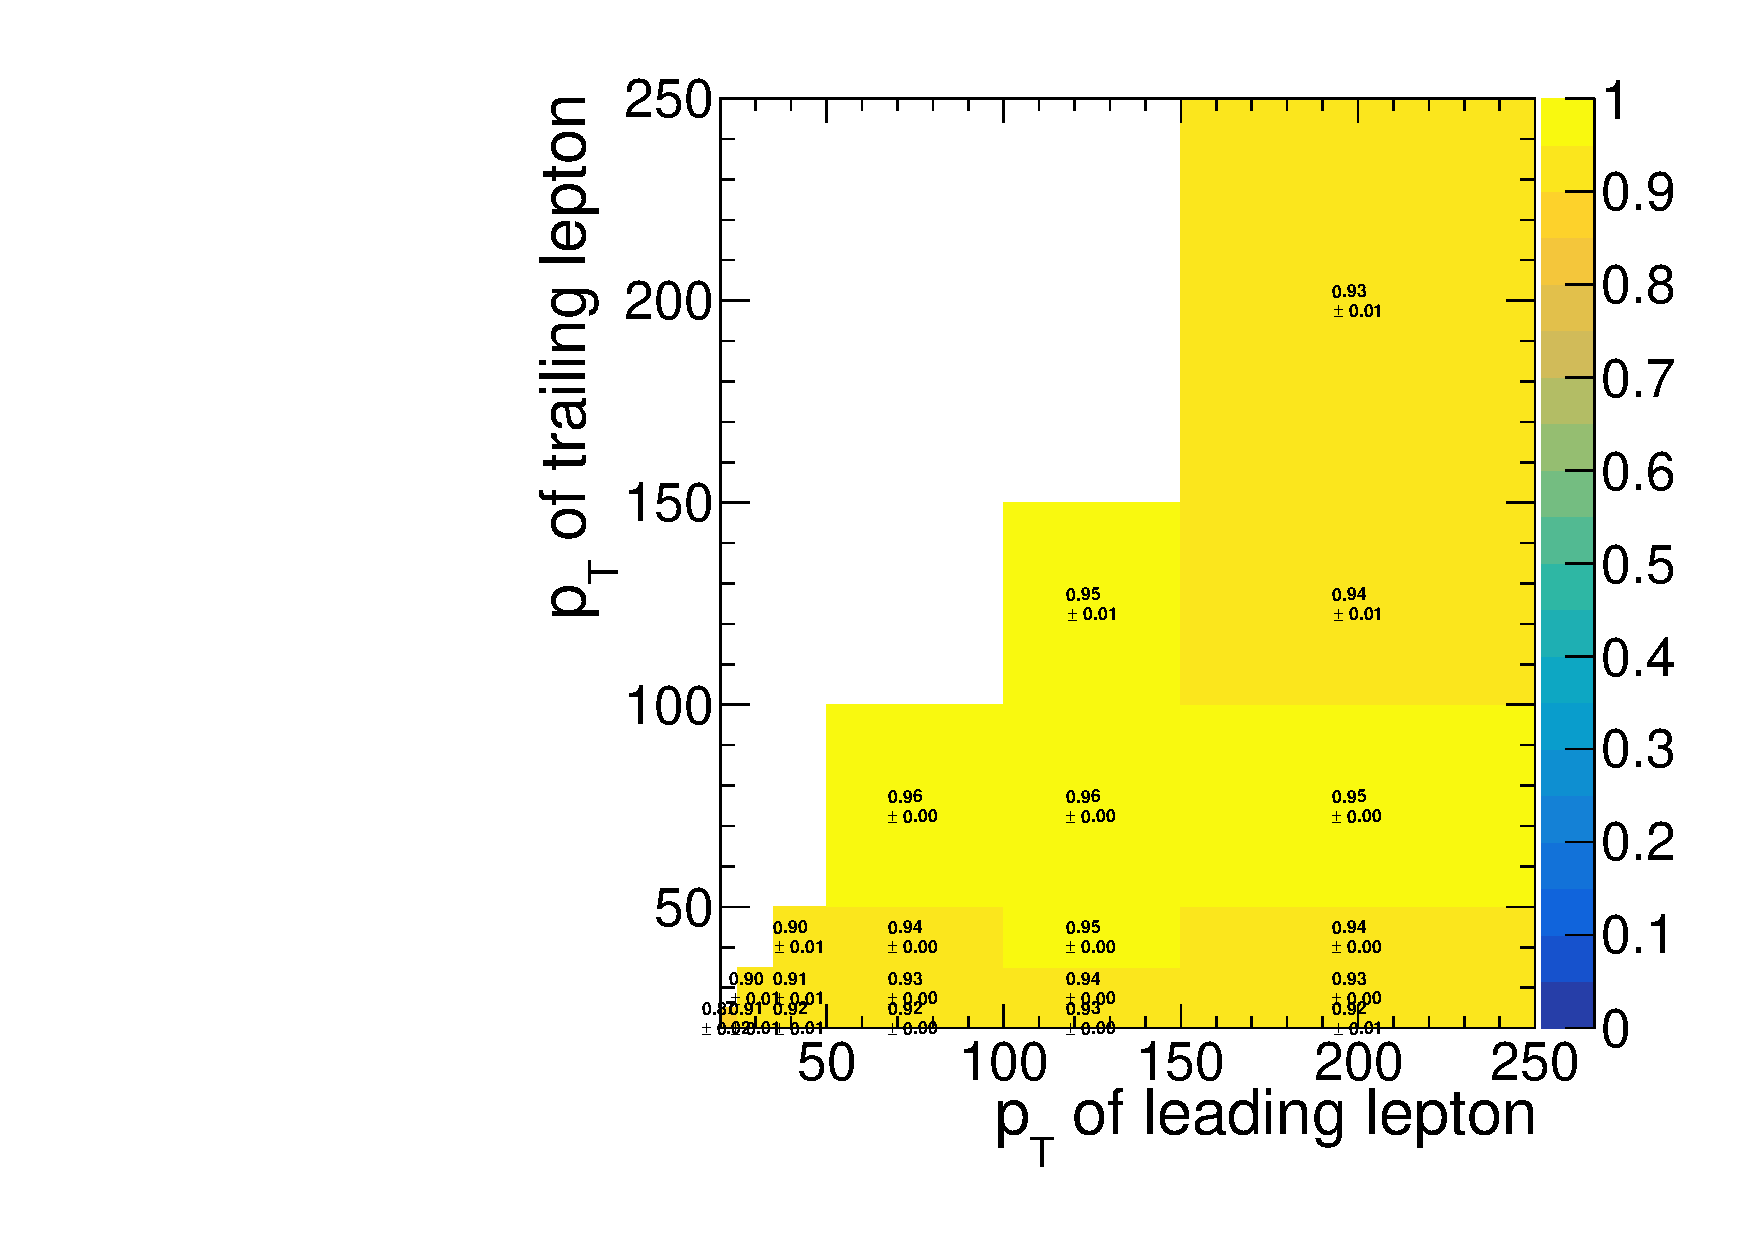
\includegraphics[width=0.5\textwidth]{figures/trigger/HLT_mumuIso_OR_HLT_mumuNoiso_OR_HLT_SingleMu_noniso_pt1_pt2_highEta1_veryCoarse_BCDEF.pdf}}
  \caption{Gain in trigger efficiency for the $\mu\mu$ channel by adding non-isolated and single-lepton triggers}
  \label{fig:additionalTriggers}
\end{figure}

We measure the trigger efficiencies in the unbiased {\verb MET } and {\verb JetHT } data sets which give consistent results. 
We use the measurement obtained in the {\verb MET } because of the smaller statistical uncertainties.
There is a significant inefficiency for muons with high transverse momentum in the muon endcaps, hence
we parametrize the trigger inefficiency as a function of the two lepton momenta and define two bins of the $\eta$ of the leading lepton that are separated by $|\eta|=1.5$. In the e$\mu$ channel, we bin the measurement in the same way but we take the $\eta$ of the muon, whether it is leading or not. 
The measured trigger efficiencies are used to scale the simulation.

Figure~\ref{fig:additionalTriggers} shows the gain in trigger efficiency by including the non-isolated double-lepton and, additionally, the single-lepton triggers for the example of the $\mu\mu$ channel and for $|\eta|>1.5$ for the leading muon. The improvement at high transverse momenta is dramatic. All other trigger efficiency maps show less prominent effects and are collected in Appendix~\ref{app:triggerEff}.

\section{Object definition and selection}

  All lepton, jet and \met objects in the event are reconstructed using the Particle Flow (PF) algorithm~\citep{CMS-PAS-PFT-09-001}.
  Jets are corrected for by {\texttt Spring16\_25nsV6} corrections and and propagated to \ETmiss (type-1 corrections). 
  \subsection{Lepton selection}
    Leptons are selected according to a set of identification and isolation criteria which are summarized in Table~\ref{leptonSelection} and discussed in the following.
    The leading lepton is required to have a transverse momentum of at least 25 \GeV, while the trailing lepton must exceed 20 \GeV.
    Both leptons must satisfy $-2.4 < \eta < 2.4$. 
    Events with additional leptons satisfying $p_T> 15$ GeV and with relative isolation below 0.4 are vetoed.

    % In case 3rd lepton is vetoed by a loose selection
\begin{table}
  \center
  \small
  \begin{tabular}{c|cc|cc}
                     & \multicolumn{2}{c|}{dilepton selection}            & \multicolumn{2}{c}{3rd lepton veto} \\
                     & electrons                   & muons               & electrons                   & muons \\
     \hline
     \pt             & $> 20\GeV$                  & $> 20\GeV$          & $> 15\GeV$                  & $>15\GeV$ \\
     $|\eta|$        & $< 2.4$                     & $< 2.4$             & $< 2.4$                     & $< 2.4$  \\ 
     isolation       & relIso03 $< 0.12$            & relIso03 $< 0.12$    & relIso03 $< 0.4$            & relIso03 $< 0.4$\\
     $|d_{xy}|$      & $< 0.05$                    & $< 0.05$            & $< 0.05$                    & $< 0.05$    \\
     $|d_{z}|$       & $< 0.1$                     & $< 0.1$             & $< 0.1$                     & $< 0.1$  \\
     SIP3D           & $< 4$                       & $< 4$               & $< 4$                       & $< 4$ \\
     identification  & cut-based tight id          & medium muon id      & cut based veto id           & veto muon id \\
                     & lostHits = 0                &                     &                             &\\ 
  \end{tabular}
  \caption{Lepton selection criteria}
  \label{leptonSelection}
\end{table}


    \subsubsection{Electron identification}
      Electrons need to pass the tight cut-based POG recommended working point in the 25ns scenario~\citep{twiki:eleId} which includes the
      requirement to pass the conversion veto. Additionally, on some identification variables we apply tighter cuts with respect to the official working point. Electron candidates 
      are only considered when they have exactly 0 missing hits. The longitudinal impact parameter $|dz|$ with respect to the primary vertex
      is required to be less than 1\mm in the endcap region ($1.479 < |\eta| < 2.4$). % Note: other impact parameters in the cut-based tight id are dxy < 0.111mm and dz < 0.466mm in the barrel and dxy < 0.351 mm; all which are tighter than our 0.5mm and 1mm
      Additionally, the significance of the 3D impact parameter should satisfy $\text{SIP}_\text{3D} \equiv \left| \frac{\text{IP}}{\sigma_\text{IP}} \right| < 4$ 
      where IP is the distance of closest approach of the lepton track to the event primary vertex and $\sigma_\text{IP}$ is its associated uncertainty. 

    \subsubsection{Muon identification}
      Muons have to pass the medium identification working point \citep{twiki:muonID}. Additionally, the transverse impact parameter $|dxy|$ and the longitudinal impact parameter $|dz|$ with respect to the primary vertex
      are required to be less than 0.5\mm and 1\mm respectively. In the same way as for electrons, the $\text{SIP}_\text{3D}$ is required to be less than 4.

    \subsubsection{Lepton isolation}
      Relative isolation smaller than 0.12 within a cone R of 0.3 around the lepton candidate is required for both electrons and muons.
      We apply the very tight (VT) multi-isolation working point to both electrons and muons. The multi-isolation approach was earlier presented in~\citep{CMS_NOTE_2015-133} and is constructed from three observables:
      \begin{itemize}
        \item the mini-isolation $I_\text{mini}$, defined as
              \begin{equation}
                I_\text{mini} = \frac{\sum_R \pt(h^\pm) + \text{max}\left(0, \sum_R \pt(h^0)+\pt(\gamma) - \rho\mathcal{A}\left(\frac{R}{0.3}\right)^2\right)}{\pt(\ell)},
              \end{equation}
              where $\sum_R\pt(h^\pm)$, $\sum_R\pt(h^0)$ and $\sum_R\pt(\gamma)$ are the sum of the transverse momentum of the charged hadrons, neutral hadrons and photons, respectively, within a cone $R$
              dependent on the lepton \pt:
              \begin{equation}
                  %R = \frac{10}{\text{min}(\text{max}(\pt(\ell), 50), 200)}
                  R = \begin{cases}
		    0.2          & \text{if } \pt < 50\GeV \\
		    10\GeV/\pt   & \text{if } 50 < \pt < 200\GeV \\
		    0.05         & \text{if } \pt > 200\GeV
                  \end{cases}
              \end{equation}
              Using a variable cone size depending on the lepton \pt ensures that the lepton is locally isolated, even in boosted topologies.
              The last term is the so-called effective area correction to mitigate the impact of pileup, where $\rho$ is the pileup energy density, % (fixedGridRhoFastJetAll)
              and the effective areas $\mathcal{A}$ used are listed in Table~\ref{table:effArea}.
              % Spring15dr POG approved areas
\begin{table}
 \begin{center}
   \small
   \begin{tabular}{lc|lc}
     $|\eta|$ range & $\mathcal{A}$(e) & $|\eta|$ range & $\mathcal{A}$($\mu$)  \\
     \hline
     $0.000-1.000$ & 0.1752 & $0.000-0.800$ & 0.0735 \\
     $1.000-1.479$ & 0.1862 & $0.800-1.300$ & 0.0619 \\
     $1.479-2.000$ & 0.1411 & $1.300-2.000$ & 0.0465 \\
     $2.000-2.200$ & 0.1534 & $2.000-2.200$ & 0.0433 \\
     $2.200-2.300$ & 0.1903 & $2.200-2.400$ & 0.0577 \\
     $2.300-2.400$ & 0.2243 & & \\
    %$2.400-2.500$ & 0.2687 & & \\
   \end{tabular}
   \caption{Effective areas used in the mini-isolation calculation for electrons and muons}
   \label{table:effArea}
 \end{center}
\end{table}

        \item the $p_T^\text{ratio}$, which is defined as the ratio of the lepton \pt and the \pt of the closest matched jet, which often contains the lepton itself. 
              If the closest jet is separated more than $\Delta R > 0.4$, then $p_T^\text{ratio} = 1$ is taken. 
              The $p_T^\text{ratio}$ variable is a simple way to identify non-prompt low-\pt leptons originating from low-\pt b-quarks, which fall outside of the mini-isolation cone.
              In order to avoid an over-correction on prompt leptons, the application of the jet energy correction is only applied on the hadronic part of the jet, using the 
              following formula at Lorentz vector level: $j = (j - PU - \ell)*JEC + \ell + PU$, where $\ell$ is the lepton, 
              $PU$ the pileup energy clustered into the jet and $JEC$ the jet energy scale correction to be applied.
        \item the $p_T^\text{rel}$ variable, defined as
              \begin{equation}
                p_T^\text{rel} = \frac{\left(\vec{p}(\text{jet})-\vec{p}(\ell)\right) \cdot \vec{p}(\ell)}{|\vec{p}(\text{jet})-\vec{p}(\ell)|}.
              \end{equation}
              which allows to recover leptons from accidental overlap with jets in boosted topologies. Similarly to $p_T^\text{ratio}$, the jet energy scale corrections are only applied on the hadronic part of
              the considered jet.
      \end{itemize}
      Using those three variables, the multi-isolation VT working point is passed when the following condition is respected:
      \begin{equation}
        I_\text{mini} < 0.09 \wedge ( p_T^\text{ratio} > 0.84 \vee p_T^\text{rel} > 7.2 )
      \end{equation}
      The logic behind this condition is that in addition to being locally isolated by $I_\text{mini}$, the lepton should carry the major part of the energy of the corresponding jet. If the $p_T^\text{ratio}$ does
      not pass the threshold, the lepton is still recovered if the overlap with the jet is accidental which is decided by the $p_T^\text{rel}$ requirement.
      For reference, the multi-isolation working points used in the SUSY group are summarized in Table~\ref{table:multiIsoWP}.
      % Multi-Iso WP 
\begin{table}
 \begin{center}
   \small
   \begin{tabular}{r|ccc}
     WP & $I_\text{mini}$ & $p_T^\text{ratio}$ & $p_T^\text{rel}$  \\
     \hline
     VL & 0.25 & 0.67 & 4.4 \\
     L  & 0.20 & 0.69 & 6.0 \\
     M  & 0.16 & 0.76 & 7.2 \\
     T  & 0.12 & 0.80 & 7.2 \\
     VT & 0.09 & 0.84 & 7.2 \\
   \end{tabular}
   \caption{Multi-isolation working points.}
   \label{table:multiIsoWP}
 \end{center}
\end{table}

    \subsubsection{Lepton selection efficiencies}
      The lepton identification and isolation efficiencies are measured per lepton leg in $Z/\gamma^*\rightarrow \ell\ell$ events using the tag-and-probe technique~\cite{twiki:SF}.
      The resulting data/MC scale factors, derived in bins of lepton \pt and $|\eta|$, have been applied on the MC and are shown in Fig.~\ref{fig:SF_e} for electrons.
      However, the efficiencies in FastSim signal samples are considerably different from those measured in fully simulated samples, due to the different modeling of showers and pileup.
      We therefore apply additional FullSim/FastSim scale factors~\citep{twiki:FSSF} on our signal samples.

      Finally, to address the issue of the loss of hit efficiency due to the Highly Ionizing Particles (HIP) an additional scale factor is applied on each of the lepton legs~\cite{twiki:HIP}.

      \begin{figure}
	\centering
	\subfloat[electron id]{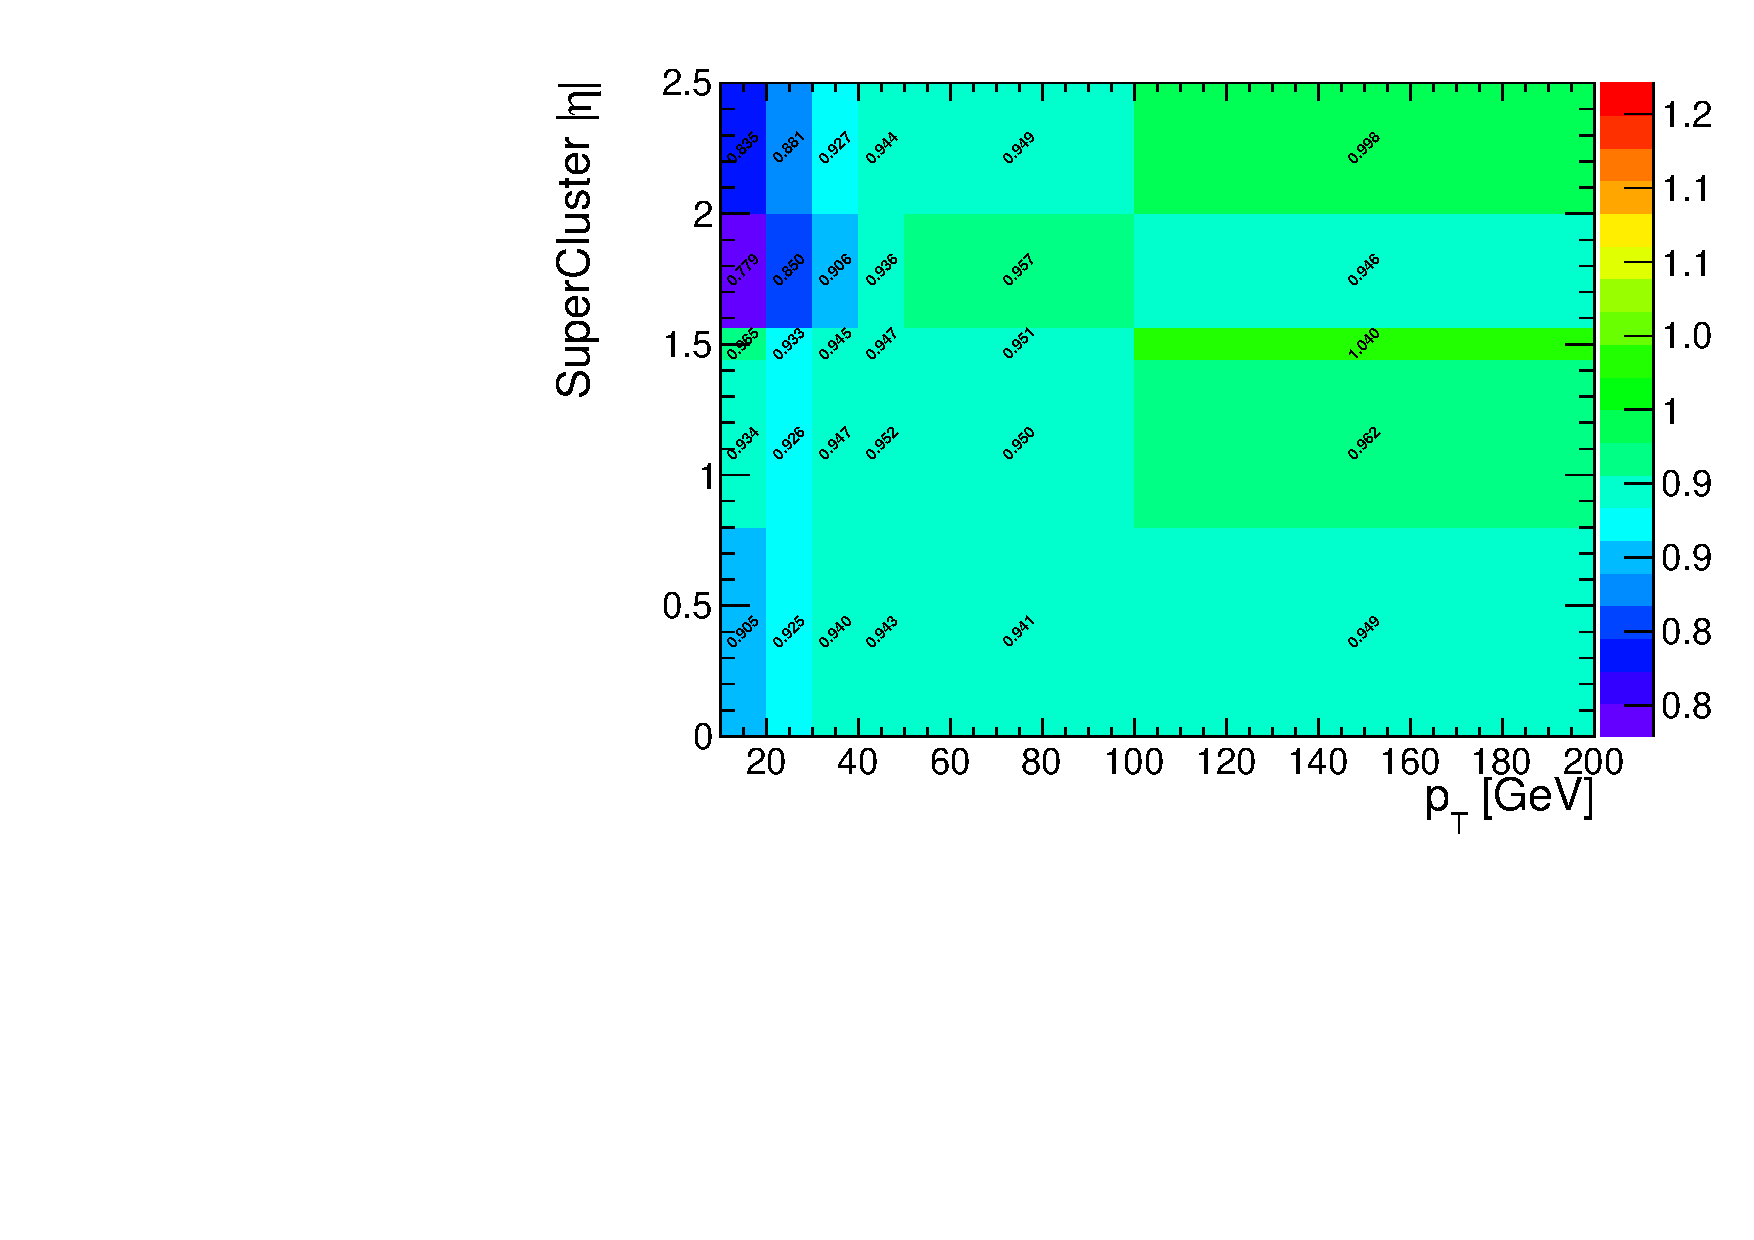
\includegraphics[width=0.45\textwidth]{figures/scaleFactors/GsfElectronToCutBasedStopsDilepton.pdf}}
	\subfloat[electron multi-isolation VT]{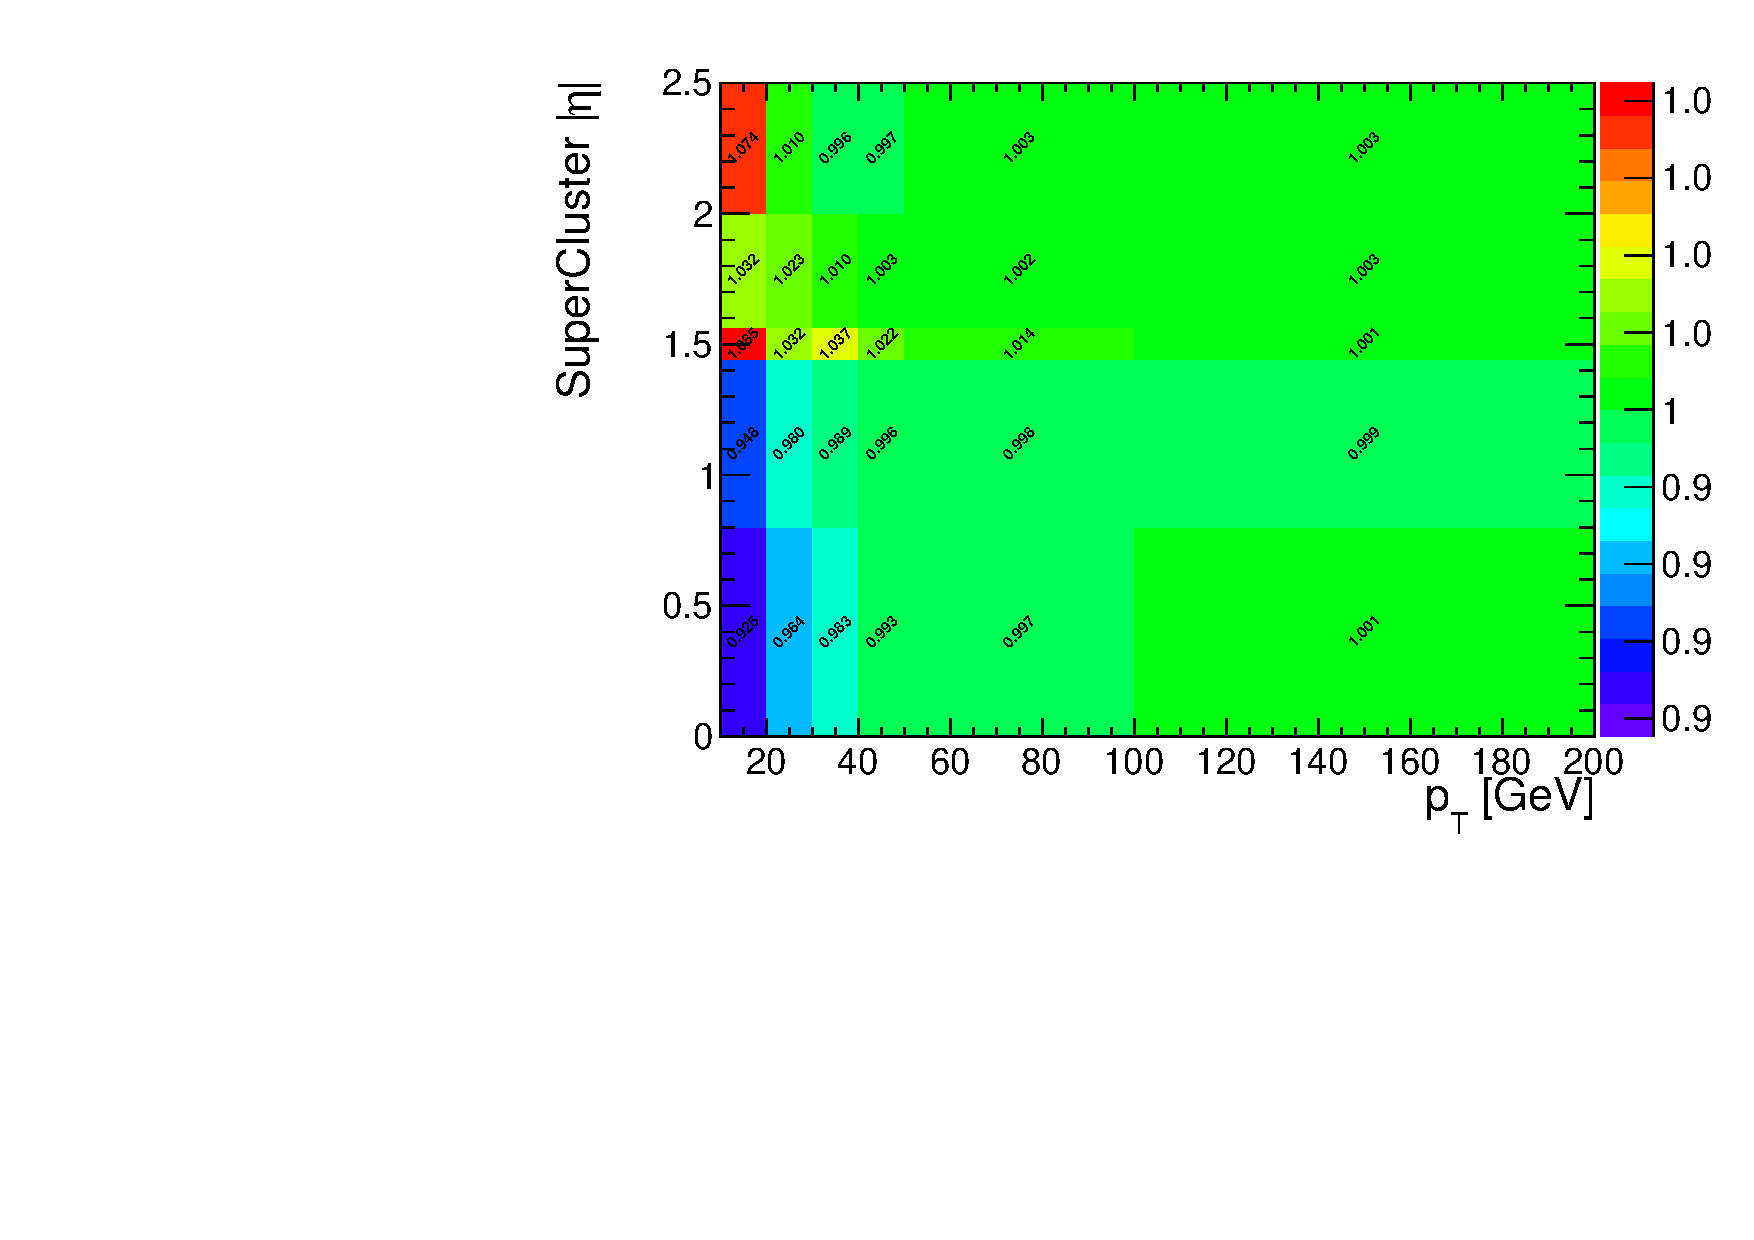
\includegraphics[width=0.45\textwidth]{figures/scaleFactors/CutBasedTightElectronToMultiIsoVT.pdf}}
	\caption{Scale factors for the identification and multi-isolation VT working point for electrons. Will be updated with final measurements.}
	\label{fig:SF_e}
      \end{figure}

  \subsection{Jet Selection}
  Particle candidates found by the PF algorithm are clustered into jets using the Anti-\kt algorithm \citep{Cacciari:2008gp} with distance parameter R = 0.4 (AK4). The influence of pileup
  is mitigated by the Charged Hadron Subtraction (CHS) technique which ignores charged particle candidates with a track closer along the $z$-axis to any vertex other than the main primary vertex. 
  Jets are calibrated in simulation and in data separately, accounting for deposits from pile-up and the imperfect detector response.
  Corrected jets with $p_{\mathrm{T}}> 30\,\GeV$ and $|\eta|<2.4$ are selected if they pass the loose jet identification criteria \citep{twiki:jetId}, i.e. the neutral electromagnetic and hadron fractions
  are $<99\%$ and the jet consists of at least two PF candidates. Furthermore, both the charged hadron fraction and multiplicity are required to be $>0$ and the charged electromagnetic fraction has to be $<99\%$.

  A selected jet may still overlap with the selected leptons.
  This is possible because the lepton can be clustered into a jet as well.
  To prevent such cases, jets that are found within a cone of $R=0.4$ around any of the selected signal leptons are  removed from the set of selected jets.

  Jets originating from the hadronization of $b$-quarks are identified using the Combined Secondary Vertex algorithm (CSVv2). The CSVv2 algorithm combines information from track impact parameters and secondary vertices identified within a given jet.
  In this analysis, a jet is $b$-tagged when its CSVv2 value passes the medium working point (\ie CSVv2 $>$ 0.800) \citep{twiki:btag}.


\begin{table}
  \center
  \small
  \begin{tabular}{|ll|}
    \hline
    \multicolumn{2}{|l|}{Event selection:} \\
    \hline
    \met filters:                                  & Flag\_HBHENoiseFilter \\
                                                   & Flag\_HBHENoiseIsoFilter \\
                                                   & Flag\_EcalDeadCellTriggerPrimitiveFilter \\
                                                   & Flag\_goodVertices \\
                                                   & Flag\_eeBadScFilter \\
                                                   & Flag\_BadMuon \\
                                                   & Flag\_badChargedHadron \\
                                                   & Flag\_globalTightHalo2016Filter \\
    \hline
    \multicolumn{2}{|l|}{$N_\text{leptons} = 2$, opposite charge} \\
    \multicolumn{2}{|l|}{$p_T(\text{lead. lep})>25$ \GeV} \\
    \multicolumn{2}{|l|}{$N_\text{jets} \geq 2$} \\
    \multicolumn{2}{|l|}{$N_\text{$b$-jets} \geq 1$} \\
    \multicolumn{2}{|l|}{$m_{ll} > 20$ GeV}\\
    \multicolumn{2}{|l|}{$|m_{ll} - m_Z| > 15$ GeV}\\
    \multicolumn{2}{|l|}{$\met > 80$ GeV} \\
    \multicolumn{2}{|l|}{$\metSig > 5 \text{GeV}^{1/2}$} \\
    \multicolumn{2}{|l|}{$\cos{\Delta\phi(\met, \text{leading jet})} < 0.8$} \\
    \multicolumn{2}{|l|}{$\cos{\Delta\phi(\met, \text{2nd leading jet})} < \cos{(0.25)}$} \\
    \hline
  \end{tabular}
  \caption{Event selection}
  \label{eventSelections}
\end{table}

\section{Control and signal regions}
 
In order to define a set of sensitive signal regions in terms of the search variables \mtll, \mtbb and \mtlblb we first exclude the
region $\mtll < 100$ \GeV which will serve as a control region and normalization region for the \ttbar background estimation.
Furthermore, the same-flavor and opposite-flavor search regions will have a different background composition because backgrounds where the two leptons
stem from a Z boson will not contribute to the opposite flavor channel. We therefore split in same-flavor (SF) and opposite-flavor (OF) regions.
 
In order to optimize the sensitivity of the analysis while ensuring reasonable statistical uncertainties in simulated samples, we defined a set of signal regions in the following way.
The region $\mtll > 100$ \GeV is sliced in bins of the other two variables starting with a relatively fine binning of 50 GeV and a large number of signal regions.
In this setting, we estimate the signal and background yields purely from simulation and produce a limit plot including all uncertainties except those related to the data-driven background estimation procedures (discussed later). Signal regions with a vanishing background estimation were excluded in this procedure as those would otherwise have biased the result towards finer binning.
Then, we collapse signal regions starting at the highest bins in each of the variables until there are no more empty regions. At each step, we re-evaluate the simulation-based contour in order
to balance small losses of sensitivity with the ensuing reduction in the number of signal regions. The process showed that a 100 \GeV binning is sufficient except for the first threshold in \mtll which should be at around 140 \GeV. We furthermore checked that splitting
the same-flavor channels into $\mu$ and e is not beneficial. The relatively small number of resulting signal regions in \mtll, \mtbb and \mtlblb is listed in Table~\ref{regions80X}. It reflects an excellent compromise between sensitivity of the analysis and feasibility of the background estimation.
 
 \begin{table}
  \center
  \begin{tabular}{c|c|c|c}
               & \mtll                          & \mtlblb                     & \mtbb \\
    \hline
    0          &                                & $0 \leq \mtlblb \leq 100$   & $70 \leq \mtbb \leq 170$ \\
    1          &                                & $0 \leq \mtlblb \leq 100$   & $170 \leq \mtbb$ \\
    2          & $100 \leq \mtll \leq 140$      & $100 \leq \mtlblb \leq 200$ & $70 \leq \mtbb \leq 170$ \\
    3          &                                & $100 \leq \mtlblb \leq 200$ & $170 \leq \mtbb$ \\
    4          &                                & $200 \leq \mtlblb$          & $70 \leq \mtbb \leq 170$ \\
    5          &                                & $200 \leq \mtlblb$          & $170 \leq \mtbb$ \\
    \hline
    6          &                                & $0 \leq \mtlblb \leq 100$   & $70 \leq \mtbb \leq 170$ \\
    7          &                                & $0 \leq \mtlblb \leq 100$   & $170 \leq \mtbb$ \\
    8          & $140 \leq \mtll \leq 240$      & $100 \leq \mtlblb \leq 200$ & $70 \leq \mtbb \leq 170$ \\
    9          &                                & $100 \leq \mtlblb \leq 200$ & $170 \leq \mtbb$ \\
    10         &                                & $200 \leq \mtlblb$          & $70 \leq \mtbb \leq 170$ \\
    11         &                                & $200 \leq \mtlblb$          & $170 \leq \mtbb$ \\
    \hline
    12         & $240 \leq \mtll$               & $0 \leq \mtlblb$ & $70 \leq \mtbb$ \\
  \end{tabular}
  \caption{Division of signal regions in bins of \mtll, \mtbb and \mtlblb}
  \label{regions80X}
\end{table}


\section{Background estimation}
\label{sec:background_estimations}
In this section, we summarize the estimation procedures for the different background components. We separately estimate the \ttbar, DY, diboson and \ttbar+Z backgrounds for
each signal region. 
  \subsection{Background estimation of \texorpdfstring{\ttbar}{ttbar}}
Similar to the 8 \TeV analysis~\cite{Khachatryan:2016pup}, the estimation of the \ttbar background estimation is based on normalizing simulated templates in a $\mtll<100$ \GeV control region.
To render this simple technique feasible, we perform a number of cross-checks in order to assess the predictivity of the simulation of both, the \mtll shoulder and the tails.

%\subsubsection{Tails in  \texorpdfstring{\ttbar}{ttbar} and in \texorpdfstring{\ETmiss}{missing energy}}
We start by investigating the tails of the \ETmiss distribution and the different tail contributions of the \ttbar background in
both simulation and in data control regions.
First, we carefully scrutinize tail contributions in simulation and then we subsequently use data control regions to assess systematically large \ETmiss mismeasurements, the impact of lepton misidentifications and
the lepton fake rate.

\subsubsection{Disentangling the tail in \texorpdfstring{\mtll}{MT2ll} in simulated events. }
\label{sec:met_tail}
It is instructive to understand the various contributions that enter the simulated \mtll tail.
We perform the checks in the \texttt{MadGraph} sample which amounts to 300/fb, i.e. each event listed below enters with a weight of 0.03 for a data set of 10/fb.
The top quark and the W boson mass endpoints are exploited by the transverse mass variables \mtll, \mtlblb, \mtbb in both single-top and top-pair production and perfectly measured top quark events are expected to populate only the low regions of these variables. 
Moreover, semi-leptonic \ttbar events with a second fake or non-prompt lepton can not enter the \mtll tail. The reason is that \ETmiss satisfies the kinematical bound of $m_T(l_1,\ETmiss)<m_W$ because there is only one neutrino in the decay, and thus,
the hypothesis $p^{\nu 2}=0$ is a possible solution in the minimization procedure in the \mtll calculation. It follows that the kinematical endpoint is also respected by semileptonic \ttbar with
fake or non-prompt leptons. Consequently, not a single event from the 300/fb madgraph \ttbar sample that was generated in the semi-leptonic channel enters any of the signal regions in either {\verb Fall15 } or {\verb Spring16 } reconstruction. 

The remaining events in the tail fall into three broad categories. First, there are drastic mismeasurements of \ETmiss which are enough to promote
an event with two leptons to the \mtll tail. This can happen either by photons or neutral particles showering in e.g. a dead ECAL crystal or by a high energetic neutrino in a jet. Second, it can happen
that a lepton in a dileptonic \ttbar event does not pass reconstruction thresholds or ID requirements and a fake or non-prompt lepton is picked up instead.
In the latter category, the decay products of one of the W's may escape detection altogether and hence provide the source for extra \ETmiss.
Finally, there are events with hadronically decaying tau leptons which have extra genuine \ETmiss.

In order to understand the impact of less isolated leptons, we loosened the isolation requirement to $I_{\text{mini}}<0.2$ hand-scanned 38 simulated events in the search region $\mtll>140$ GeV
in {\verb Fall15 } samples. There were 5 events were found in the $\mu\mu$ channel, 11 in the $ee$ channel and 22 in the $e\mu$ channel.
The 19 events with mismeasured jets are distributed approximately independently of lepton flavor and 11 have highly energetic photons or pions showering in dead ECAL cells. 
One event in this category have two jets mismeasured.
We traced the generated particles individually and correlated their disappearance with known cracks in the detector. It is noteworthy, that the current simulation (Spring16)
correctly simulates all calorimetry dead cells. The remaining 8 events each had a neutrino produced inside a jet in excess of 40 GeV which is enough to promote the event to the tail. 
We checked that by treating the neutrino momentum as visible energy, the value for \mtll is in  the bulk of the \mtll distribution. In one extreme case, a 1.6 \TeV b-jet produced a 200 \GeV neutrino.
Another source is due to either lost electron (muon) or a hadronically decaying  tau lepton from one of the W-bosons combined with a non-prompt or fake lepton passing the lepton selections.
In such events a lepton from a W and a fake lepton are used to compute the \mtll and the resulting value does not respect to the W transverse mass endpoint anymore. 
There were 12 events involving a $\tau$ lepton of which 3 decayed leptonically. An overview of the situation from gen-level (top) to reco-level (bottom) is given in Fig.~\ref{fig:ttbar_tail}.

The study was repeated in {\verb Spring16 } with the nominal isolation requirement showing a reduction of the fake and non-prompt lepton component and compatible results on the \ETmiss related backgrounds. Results on event by event basis are listed in Tab.~\ref{tab:80Xtail}. 
\begin{table}
  \center
  \small
  \begin{tabular}{l|l|l}
  & event:run:lumi & result \\ 
  \hline 
0  &  1:4953:3991364    & gamma lost in dead cell (jet mism.)\\
1  &  1:5468:4532888    & jet mismeasurement at $\eta/\phi=$ -0.934/2.9678\\
2  &  1:6024:4854452    & $\gamma$ lost at $\eta/\phi=$ 1.6/-2.4, 1.9/2.7 small jet mism., $\nu$ from jet\\
3  &  1:6171:4972344    & jet mismeasurement (Ecal), 160 \GeV \\
4  &  1:12852:10356846  & lost $K^{+}$ at $\eta/\phi=$ 1.391/-2.527\\
5  &  1:13923:11219847  & looks like jet mismeasurement, no AOD available\\
6  &  1:17046:13736425  & gaussian jet mism., $\nu$ in jet \\
7  &  1:18692:15495640  & 40\GeV overmeasured $\mu$ at $\eta/\phi=$ 2.287/-0.282, jet mism.\\
8  &  1:20840:17276057  & lost high pt $\gamma$ at $\eta/\phi=$ -1.5/0.6 (jet mism.), $\nu$ in jet\\
9  &  1:25322:20991689  & $\nu$ in a jet of 100\GeV, just passing the threshold (142\GeV)\\
11 &  1:27005:21762195  & lost $\gamma$ and neutrals in dead cell $\eta/\phi=$ 1.152/-3.077 (jet mism.)\\
12 &  1:40541:33607796  & lost $\mu^-$ from W, picked up $e^-$ fake, \\&&some trk inefficieny at $\eta/\phi=$ -2.175/0.183 (seems gaussian)\\
13 &  1:48624:40308549  & lost high pt $\gamma$ (jet mism.)\\
14 &  1:49599:41117351  & lost mu- in a jet $\eta/\phi=$-0.999/0.558 \\
15 &  1:51330:42552044  & lost energy in ECAL (jet mism.) $\eta/\phi=$-0.837/2.890\\
16 &  1:57932:48024871  & fake $\mu$ at $\eta/\phi=$ 0.289/-2.763, also gaussian jet mismeasurement \\
17 &  1:62587:51884514  & jet mism. in a 200\GeV genjet, $\nu$ in another jet\\
18 &  1:65097:53964677  & lost $\mu$ to pt cut, picked up fake e from conversion $\gamma$,\\&& plus jet mism. (gaussian) \\
19 &  1:67998:56369604  & $\nu$ from jet\\
20 &  1:68445:56740873  & $\tau$ decaying hadronically, non-prompt $\mu$\\
21 &  1:71016:58872109  & fake $\mu$ with 60 \GeV inconsistency btw inner track and global track\\
22 &  1:72622:60203349  & $\nu$ in jet, several $\gamma$ lost in jet\\
23 &  1:74317:61608051  & 30 \GeV $\mu$ mism. at $\eta/\phi=$-2.275/-1.514\\
24 &  1:82880:68707320  & likely non-prompt $\mu$, no AOD available\\
25 &  1:85837:71158655  & $\nu$ from jet\\
26 &  1:94223:78110867  & $\gamma$ lost in crack\\
27 &  1:106121:87973932 & several mism. jets\\
28 &  1:113723:94275792 & jet mismeasurement at $\eta$ approx. 3, $\nu$ in a jet
  \end{tabular}
  \caption{Result of the tail scan of \ttbar in \texttt{Spring16} simulation.}
  \label{tab:80Xtail}
\end{table}


\begin{figure}[!hbtp]
\centering
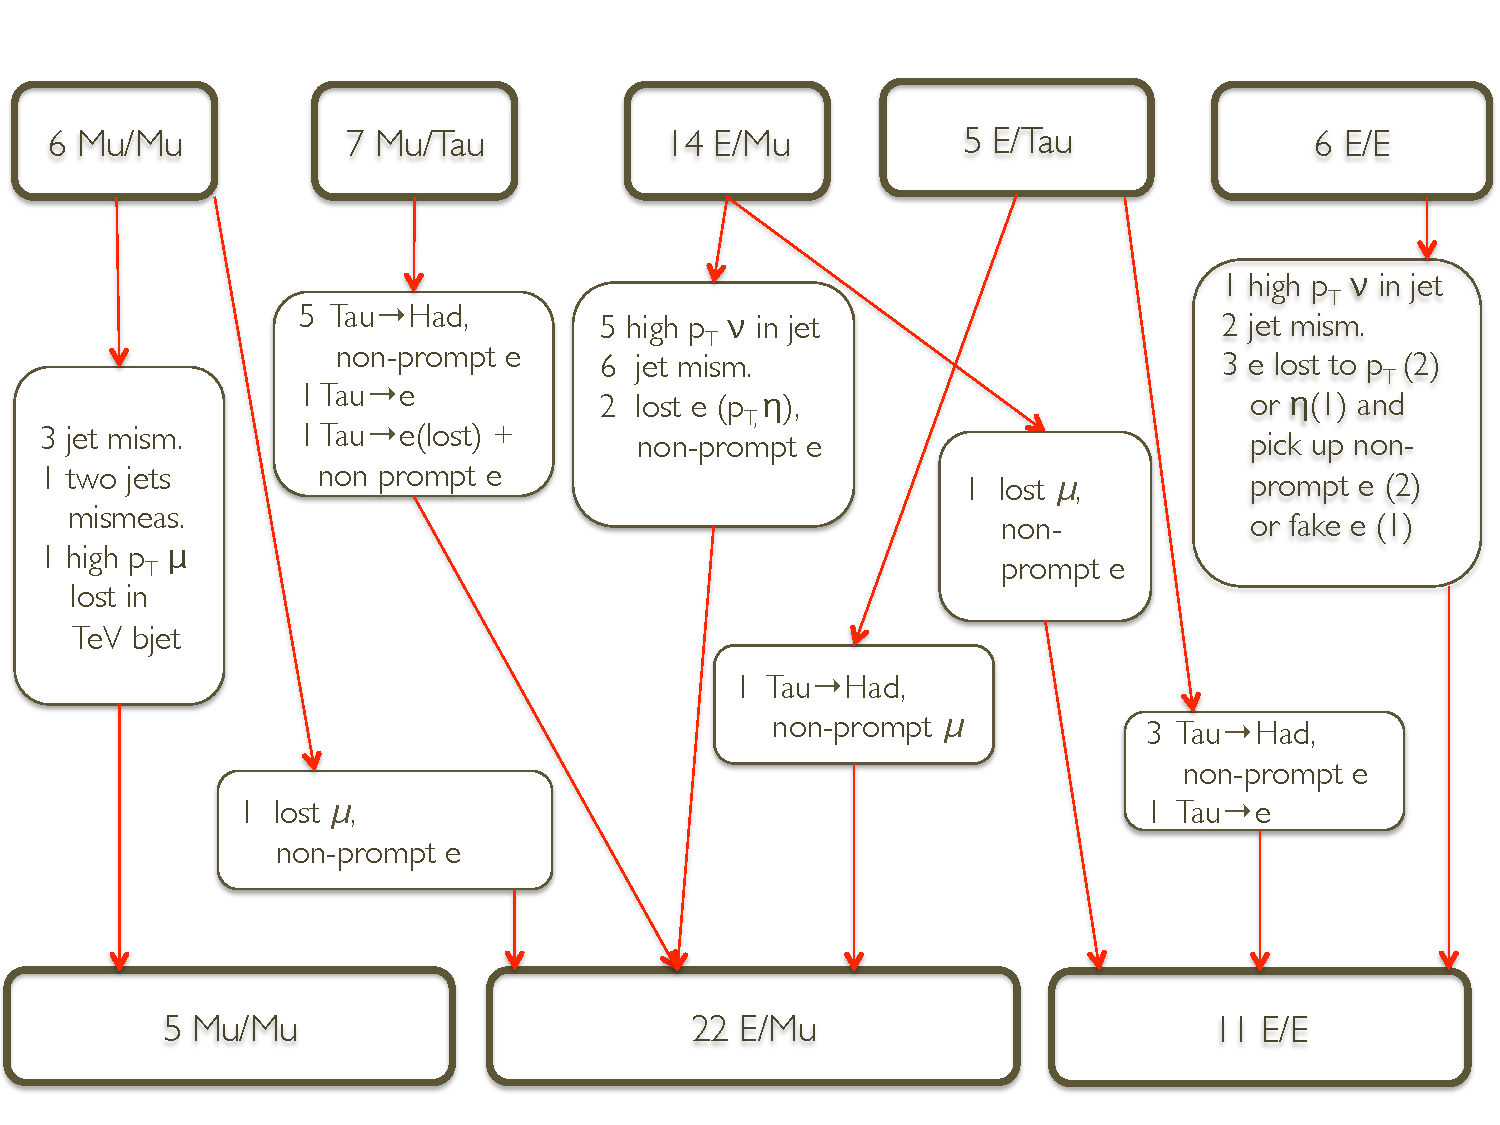
\includegraphics[width=0.9\textwidth]{figures/ttBar/ttbar_tail.pdf}
\caption{Overview of 38 events passing $\mt2ll>140$ GeV. Gen-level is at the top, reco-level at the bottom.}
\label{fig:ttbar_tail}
\end{figure}

Data control regions are formed to validate MC simulation for these sources and results are presented in the following sections.

\subsubsection{ Check of \ETmiss tails in DY data }

\begin{figure}[!hbtp]
\centering
\subfloat[]{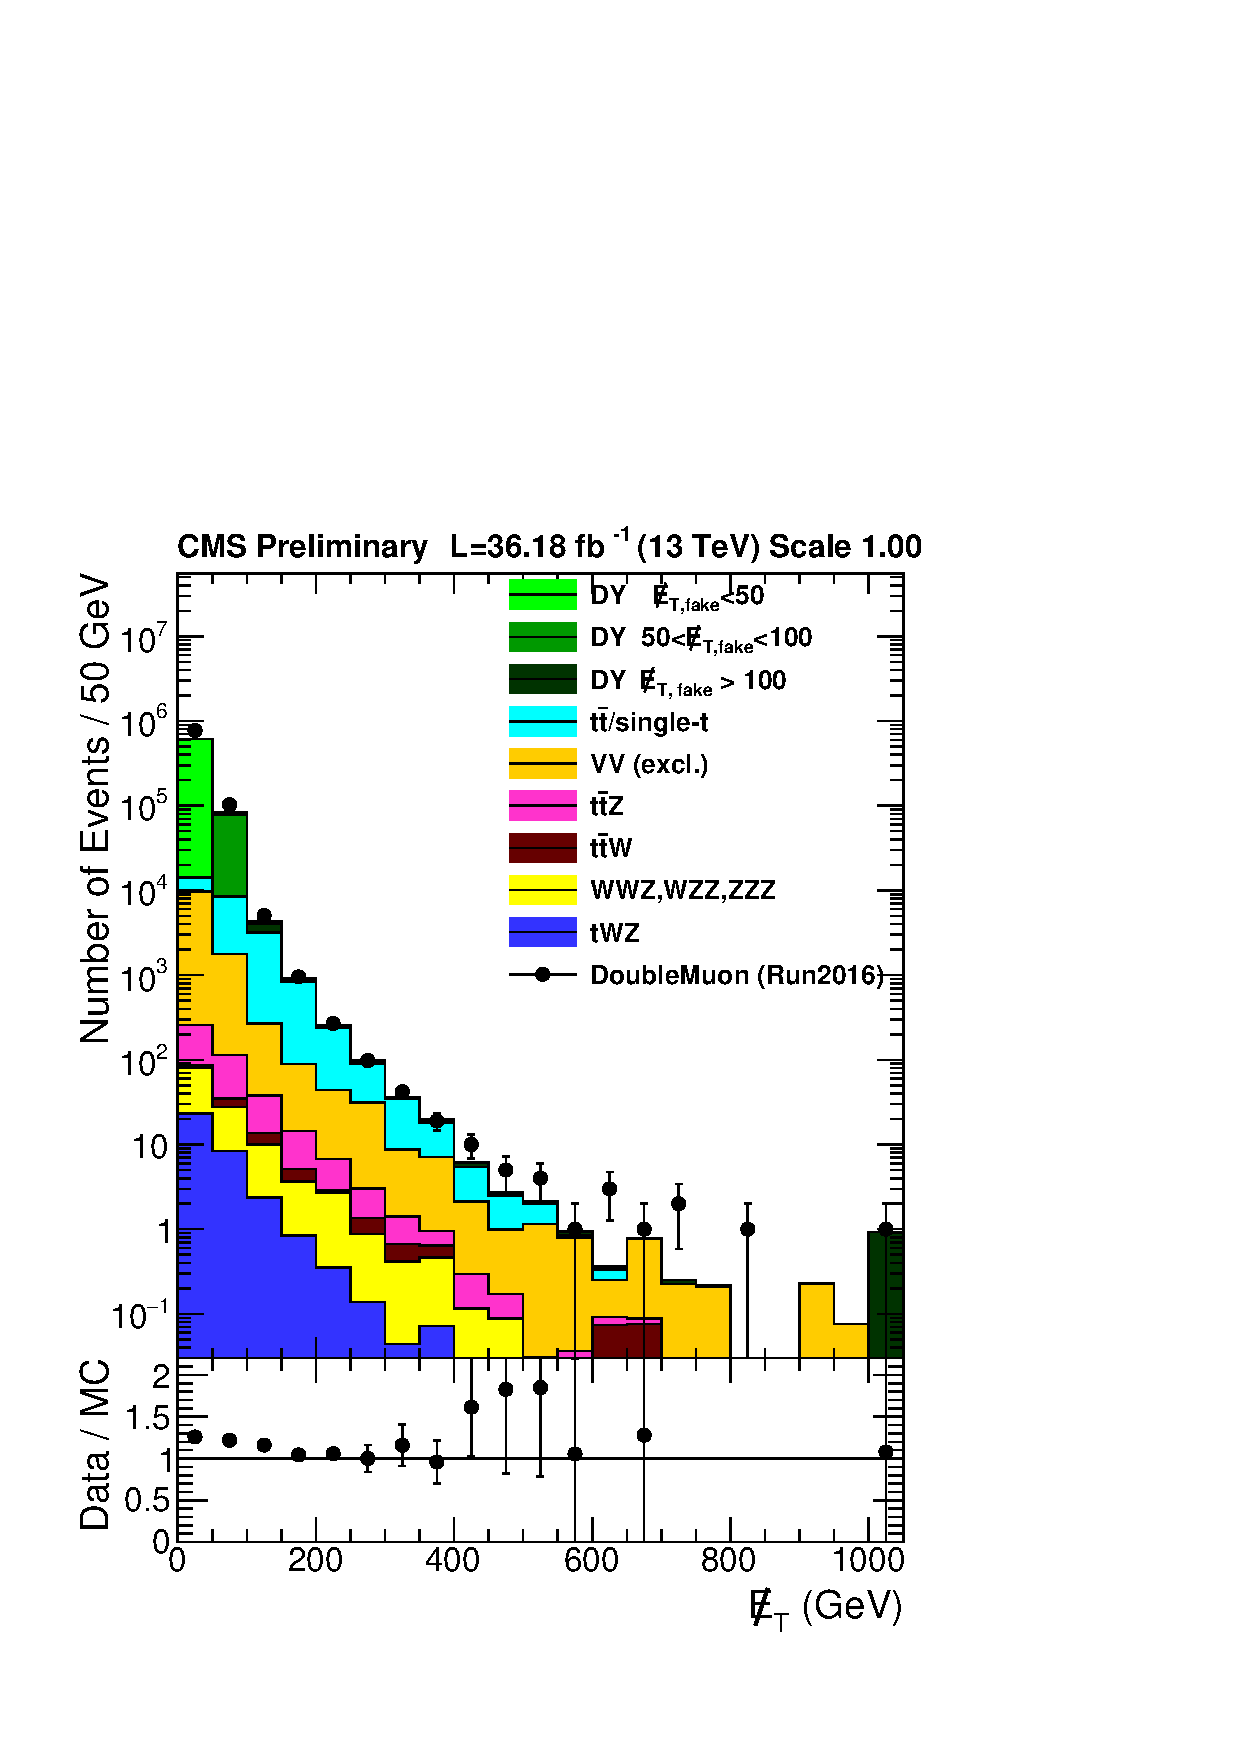
\includegraphics[scale=0.45]{figures/ttBar/met_control_met_pt_v2.pdf}}
\subfloat[]{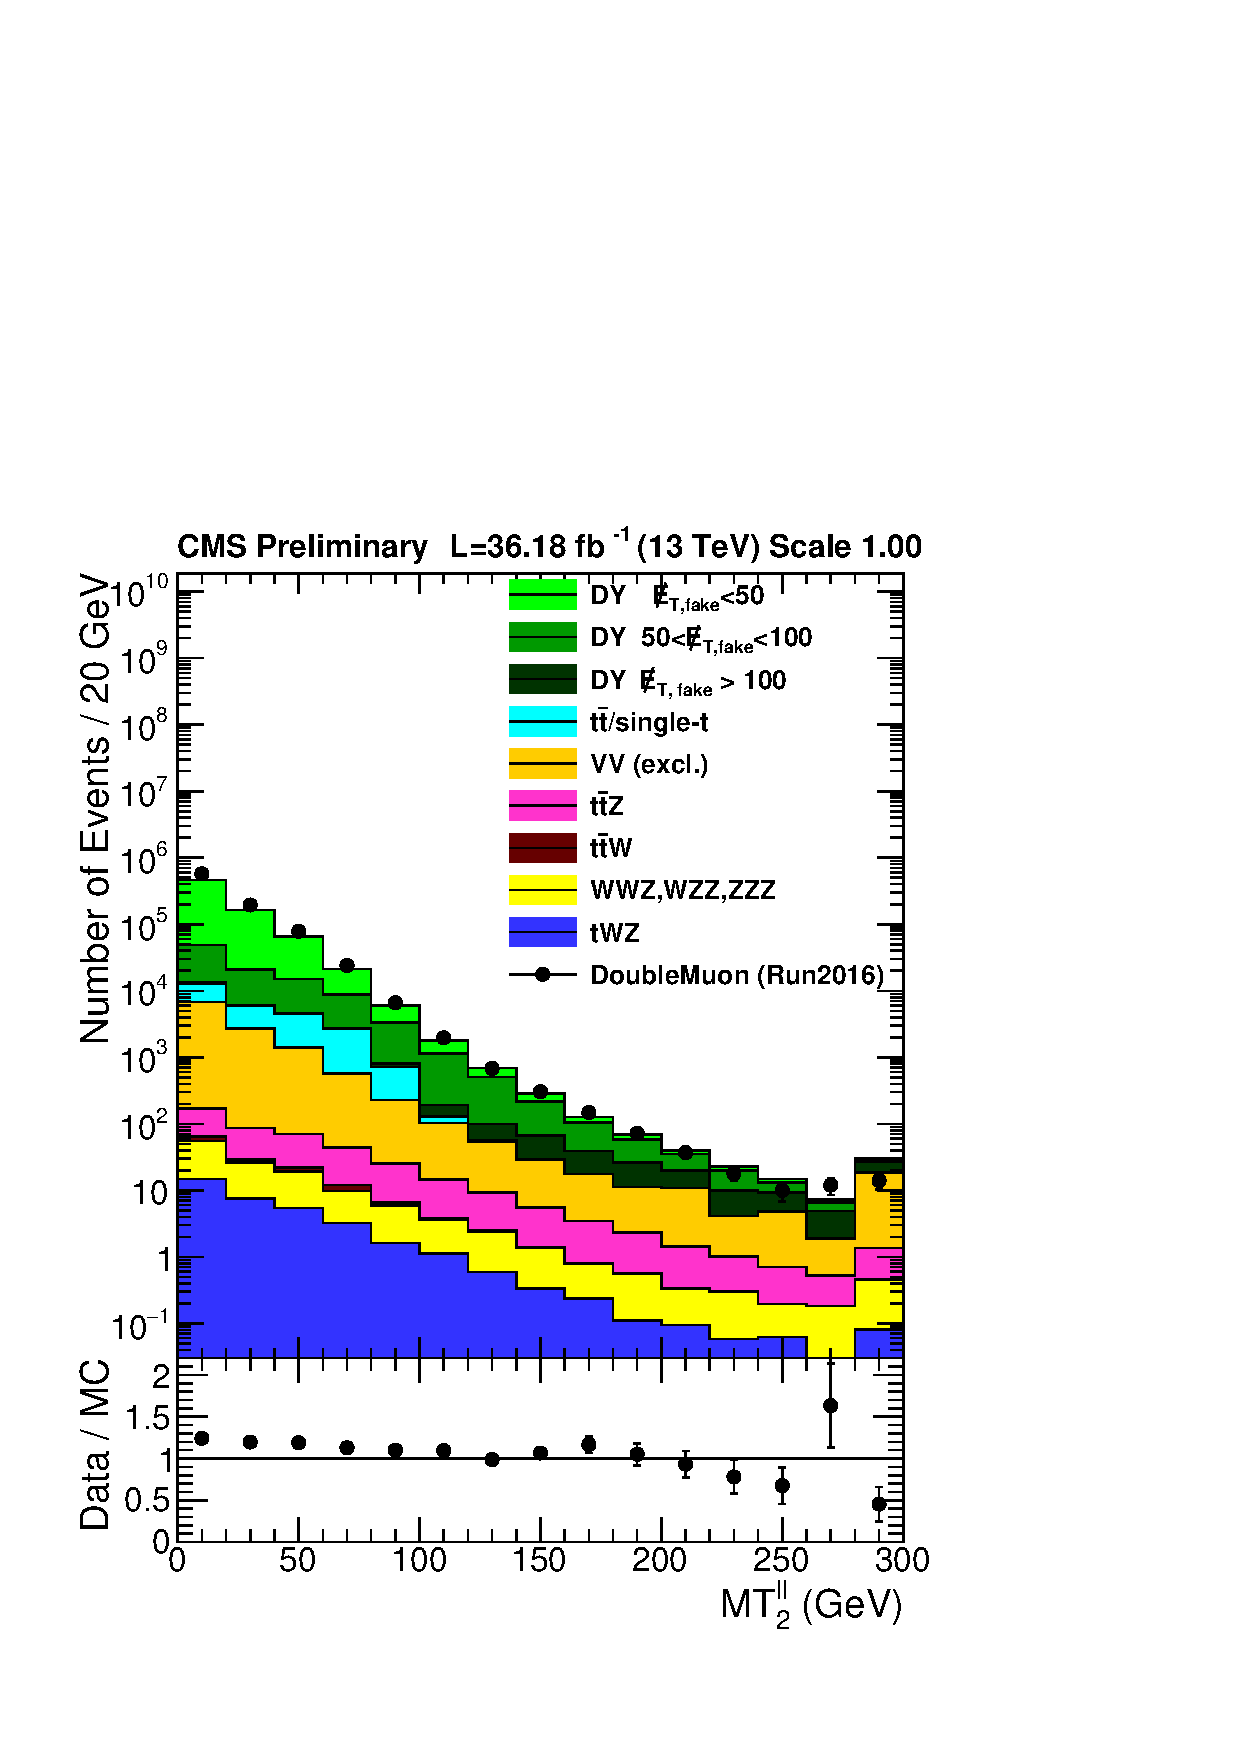
\includegraphics[scale=0.45]{figures/ttBar/met_control_dl_mt2ll_v2.pdf}}
\caption{ \ETmiss and \mtll distribution in the on-Z selection with 0 b-tags.}
\label{fig:met_tail_controlPlots}
\end{figure}

We proceed to check whether there is a sign of a higher rate of drastic jet mismeasurements in data. We can do that again in the 0 b-tag on-Z region selecting events
with zero genuine \ETmiss. The \ETmiss distribution is shown in Fig.\ref{fig:met_tail_controlPlots}a and the high \ETmiss tail is populated by \ttbar which, on the contrary, does predict genuine 
\ETmiss. In order to perform a sensible check anyways, we first split the DY sample in three bins of fake \ETmiss at thresholds of 50 \GeV and 100 \GeV shown in different shades of green.
Then, we exploit the excellent suppression of \mtll of dileptonic ttbar. The \mtll distribution is shown in Fig.\ref{fig:met_tail_controlPlots}b and shows that for $\mtll>100 \GeV$ the 
data is dominated by DY with large mismeasurements and that apparently there is no significant excess of events with jet mismeasurements.

\subsubsection{ Shape analysis of fake lepton backgrounds }

\begin{figure}[!hbtp]
\centering
\subfloat[Three-lepton control region]{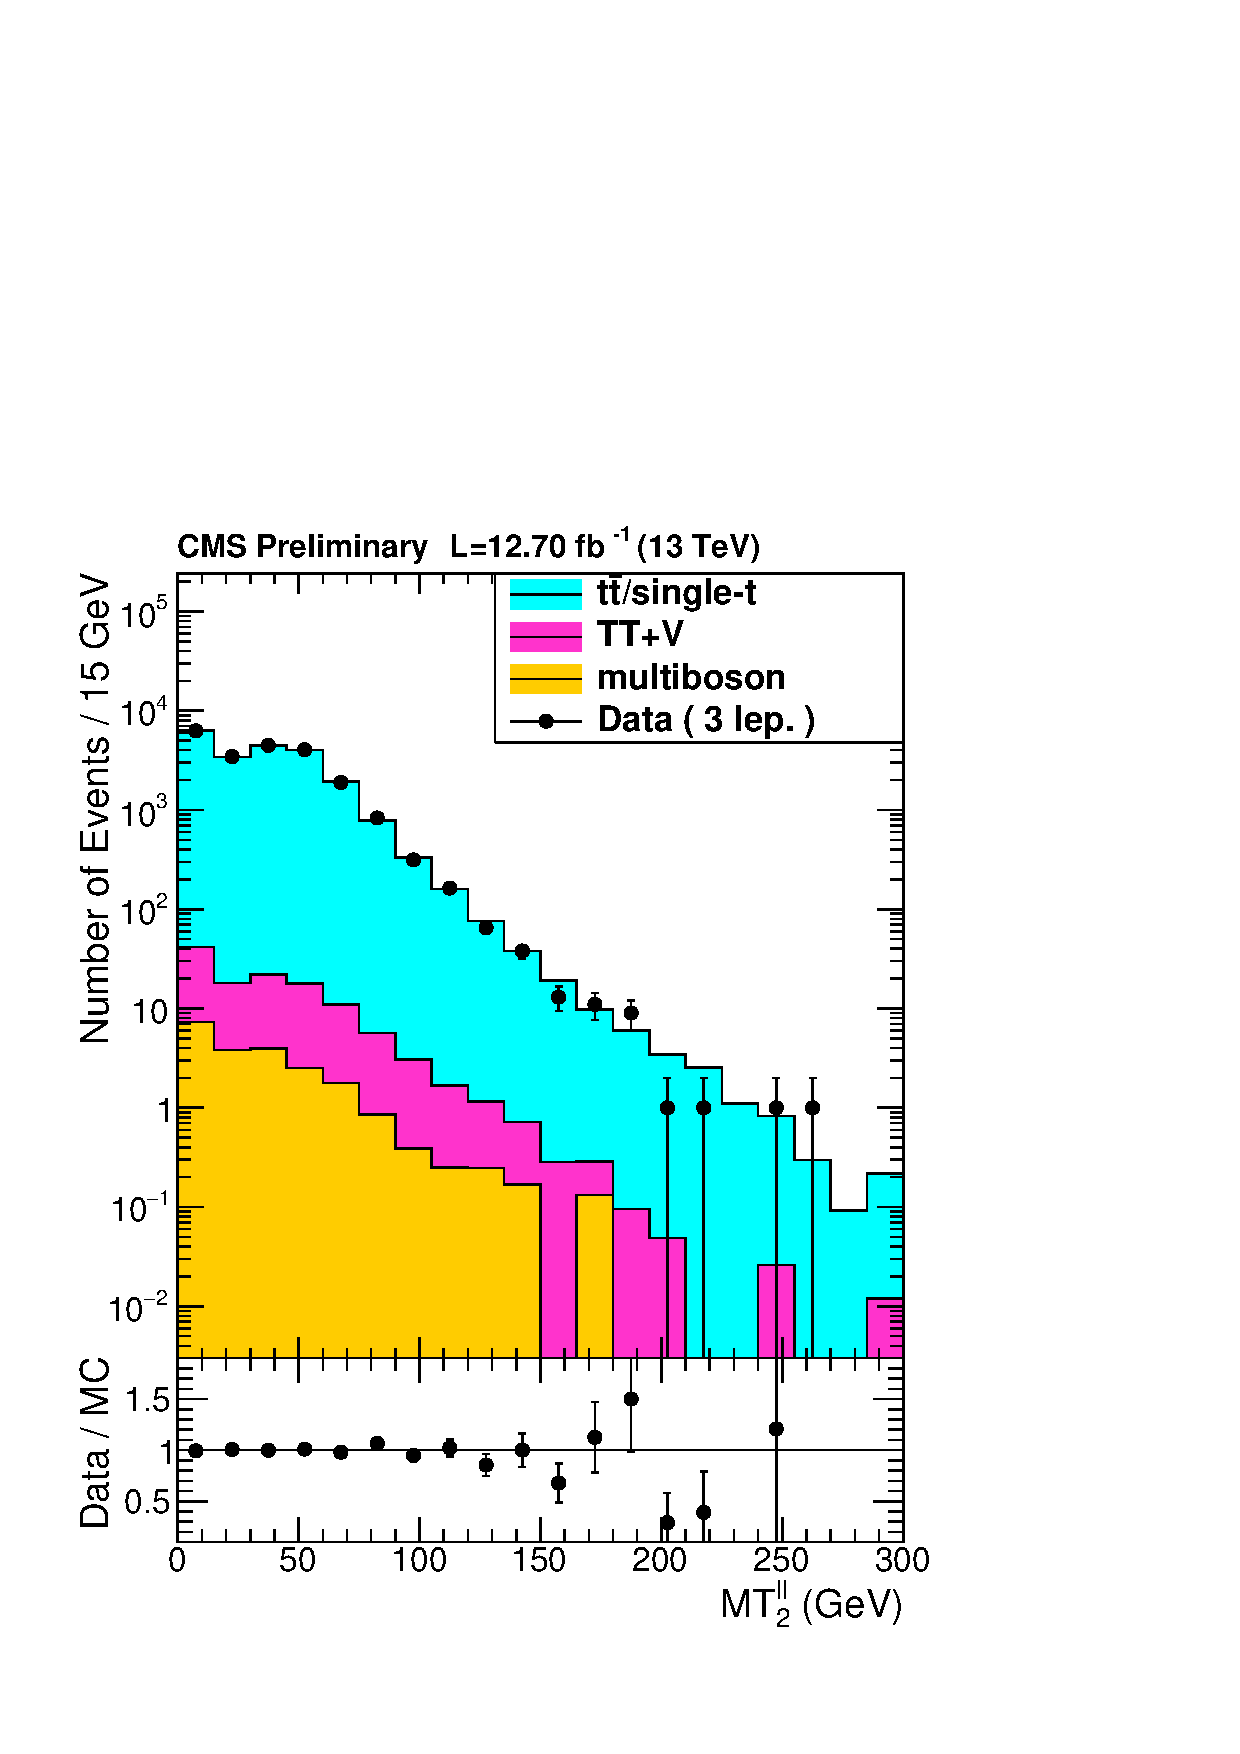
\includegraphics[width=0.35\textwidth]{figures/ttBar/all_dl_mt2ll.pdf}}
\subfloat[\ttbar 2l vs. 3l]{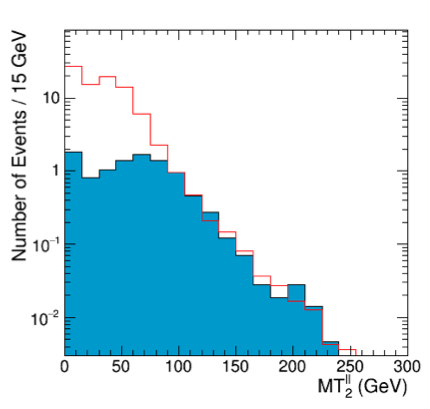
\includegraphics[width=0.5\textwidth]{figures/ttBar/MC_fake_shape_comparison.png}}
\caption{Left: \mtll distributions in two control regions enriched by $t\bar{t}$ events. MC yields are normalized to data using the yields at $\mtll<100$ \GeV. Right: Comparison of the three lepton simulation (blue area) 
and the two-lepton simulation with inverted isolation requirements on one lepton (red line), normalized at $\mtll>100$~\GeV. \FIXME{Robert, please update.}}
\label{fig:ttBar_3l}
\end{figure}

Next, we check whether the \mtll shape is correctly simulated. To this wend, we mimic lepton mis-identification by selecting three lepton events where the third lepton is selected with very loose requirements. 
%All other selections summarised in Table ~\ref{Tab:baselineSel} are applied. 
In order to imitate the loss of a lepton, we recompute \mtll by combining either the leading or the sub-leading lepton with the extra trailing lepton selected in this way.
We keep track of the changes in flavor channel associated with the lepton replacement.
This swapping procedure is applied to lepton momenta only, the \ETmiss is not changed because of the very high detection efficiency and compensating nature of the nearly hermetic CMS detector.
The procedure can be applied to both data and simulation and the resulting \mtll distribution is shown in Figure~\ref{fig:ttBar_3l}a and exhibits excellent agreement between data and simulation.

It remains to be shown that the swapping procedure really mimics the lost lepton contribution. This is done in Figure~\ref{fig:ttBar_3l}b where we overlay the two-lepton simulation with an inverted
isolation requirement $I_{\text{mini}}>0.2$ on the trailing lepton (red line) with the three-lepton prediction from the swapping procedure (blue area). 
The distributions are normalized for $\mtll>100$~\GeV and the almost perfect agreement confirms that the swapping procedure mimics the loss of a lepton very well for $\mtll>80$~\GeV. 
It should be noted that the swapping
procedure is not strongly dependent on the details of the selection of the extra leptons. As long as the loose selection guarantees that extra leptons are dominated by non-prompt decays in b-jets,
the reconstructed value of \mtll is governed by the relative angular position of the extra lepton and less by it's transverse momentum which is typically too small to have a very large effect.
We conclude that there are no signs of a discrepancy in the \mtll shape for events with a lost lepton.

\subsubsection{ Check of the lepton fake rate }
In order to verify that also the rate of fake leptons that enter in our selection is well modeled by MC we selected 3-lepton events where the two of the leptons are selected with tight requirements (same as in the analysis) and the 3${}^{\text{rd.}}$ lepton with a transverse momentum threshold of 10 GeV and relaxed isolation requirement. 
In addition, we ask $\Njets\geq2$ and $\Nbtags\geq1$ to select a similar phase space. No \ETmiss or \metSig requirements made. In this selection we check the distribution of $I_{\text{rel.mini}}$ and the standard relative isolation $I_{\text{rel}}$. 

\begin{figure}[!hbtp]
\centering
\subfloat[ $\mu\mu\mu$ ]{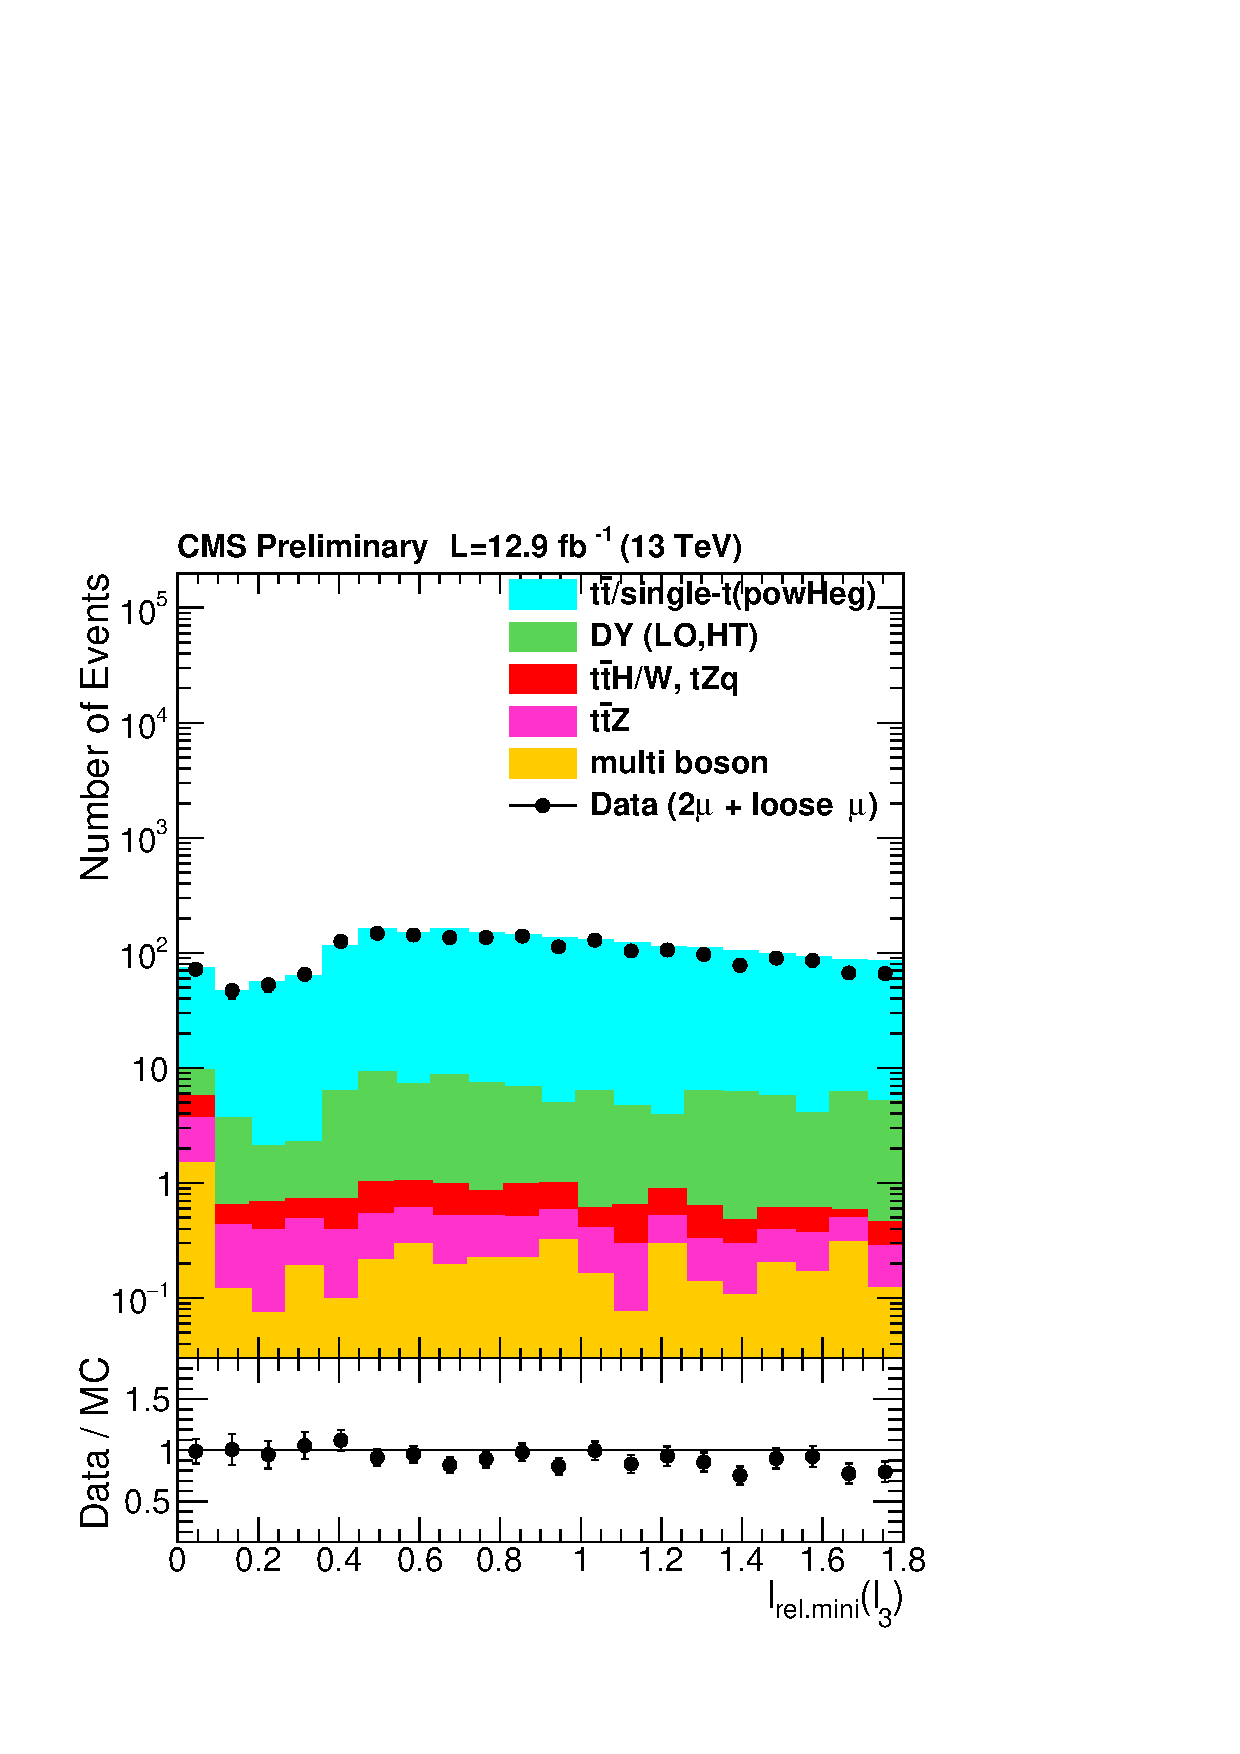
\includegraphics[scale=0.45]{figures/fakeRate/mumu_loose_mu_log/njet2-btagM-multiIsoWP/l3_miniRelIso.pdf}}
\subfloat[ eee ]{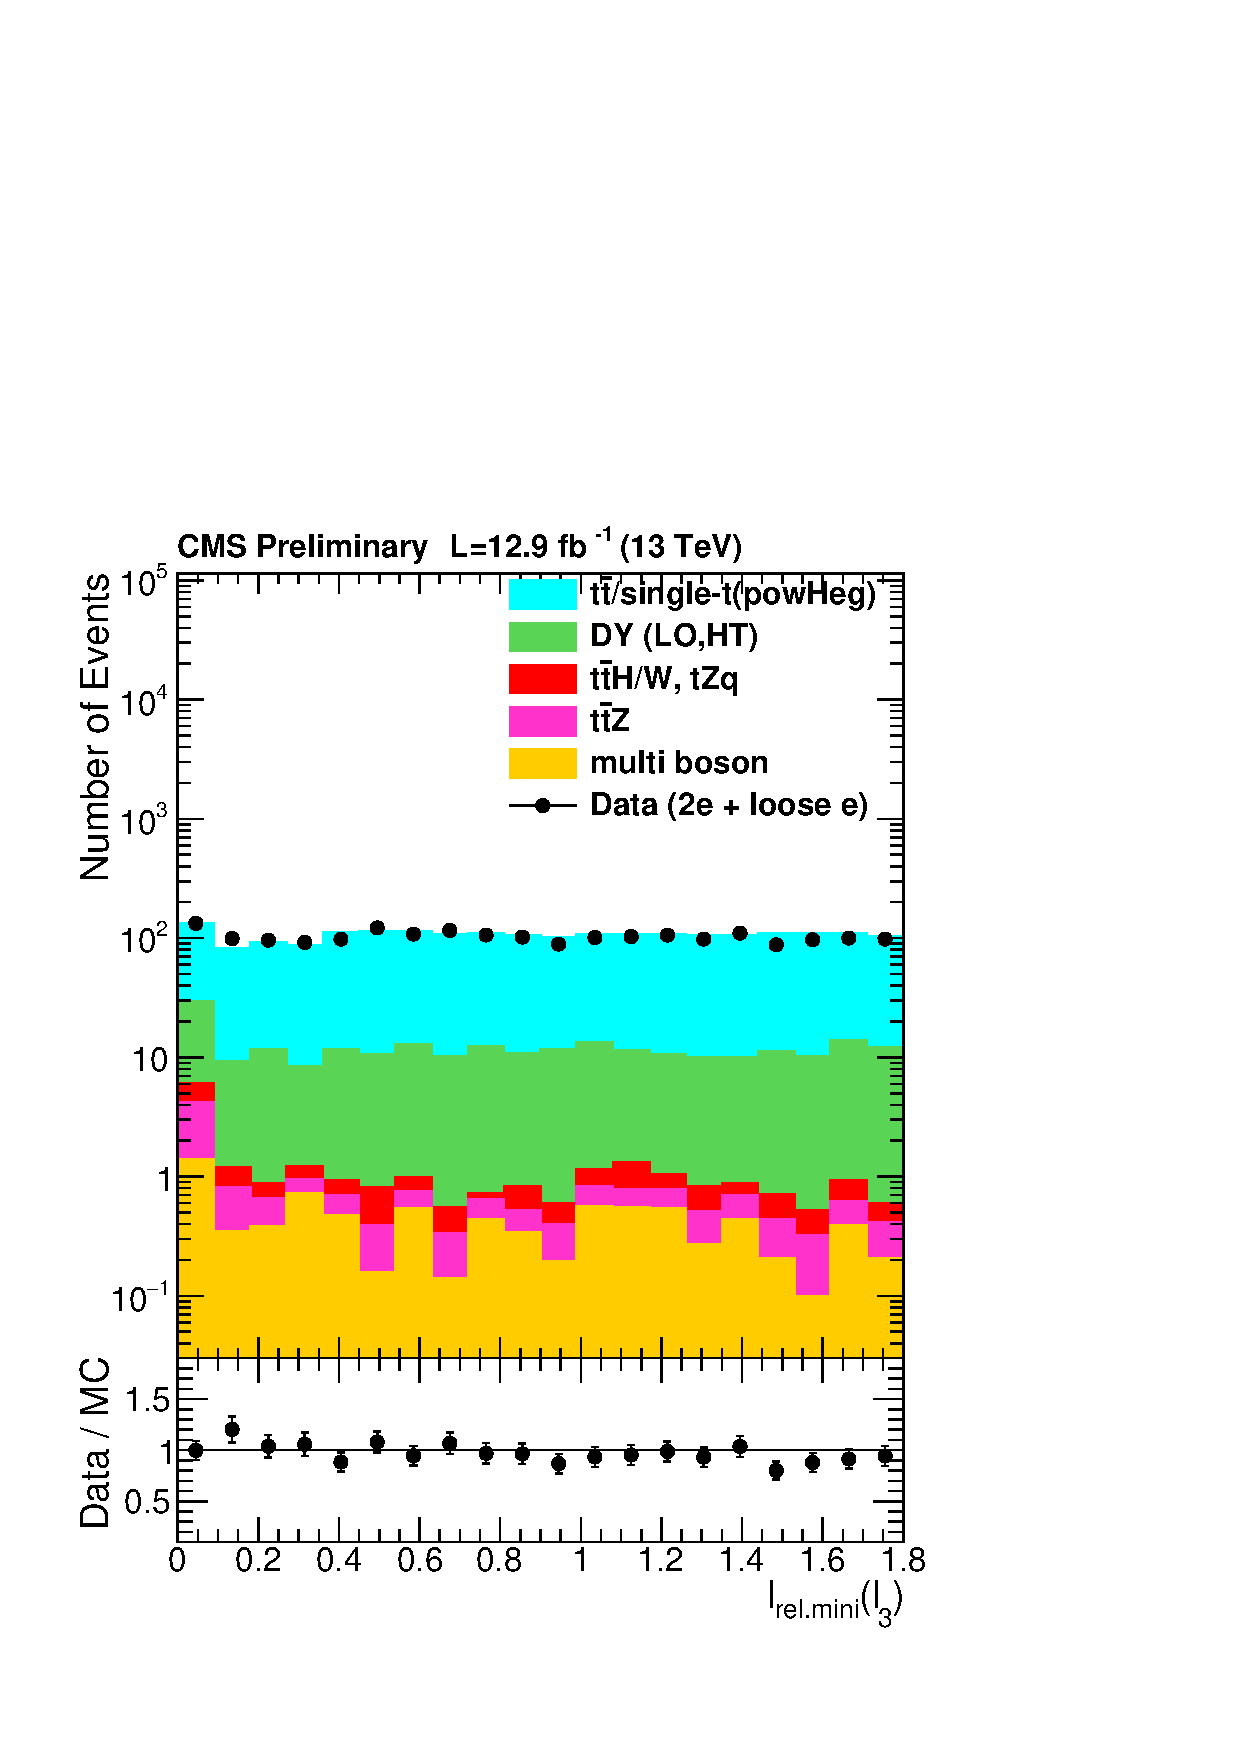
\includegraphics[scale=0.45]{figures/fakeRate/ee_loose_e_log/njet2-btagM-multiIsoWP/l3_miniRelIso.pdf}}
\caption{ $I_{\text{rel.mini}}$ and $I_{\text{rel.}}$ distribution of the third non-isolated lepton in the $\mu\mu\mu$ (left) and eee (right) channels. \FIXME{Tom, please update.}}
\label{fig:ttBar_FR_controlPlots}
\end{figure}

The distributions in Fig.\ref{fig:ttBar_FR_controlPlots} are normalized to luminosity. 
The fake-rate can be derived from the ratio of the first bin to the rest of the distribution. 
From the reasonably good agreement between data and simulation for the shape of the distributions, we conclude that the FR in data matches the one in MC. 
Nonetheless, we deduce an 15\% uncertainty driven by the available statistics in the first bins.

\subsubsection{ Validating the \texorpdfstring{\ttbar}{ttbar} shape in control regions at high and low \ETmiss}

\begin{figure}[!hbtp]
\centering
\subfloat[ $\Njets \leq 1$, $\Nbtags=0$, high \ETmiss]{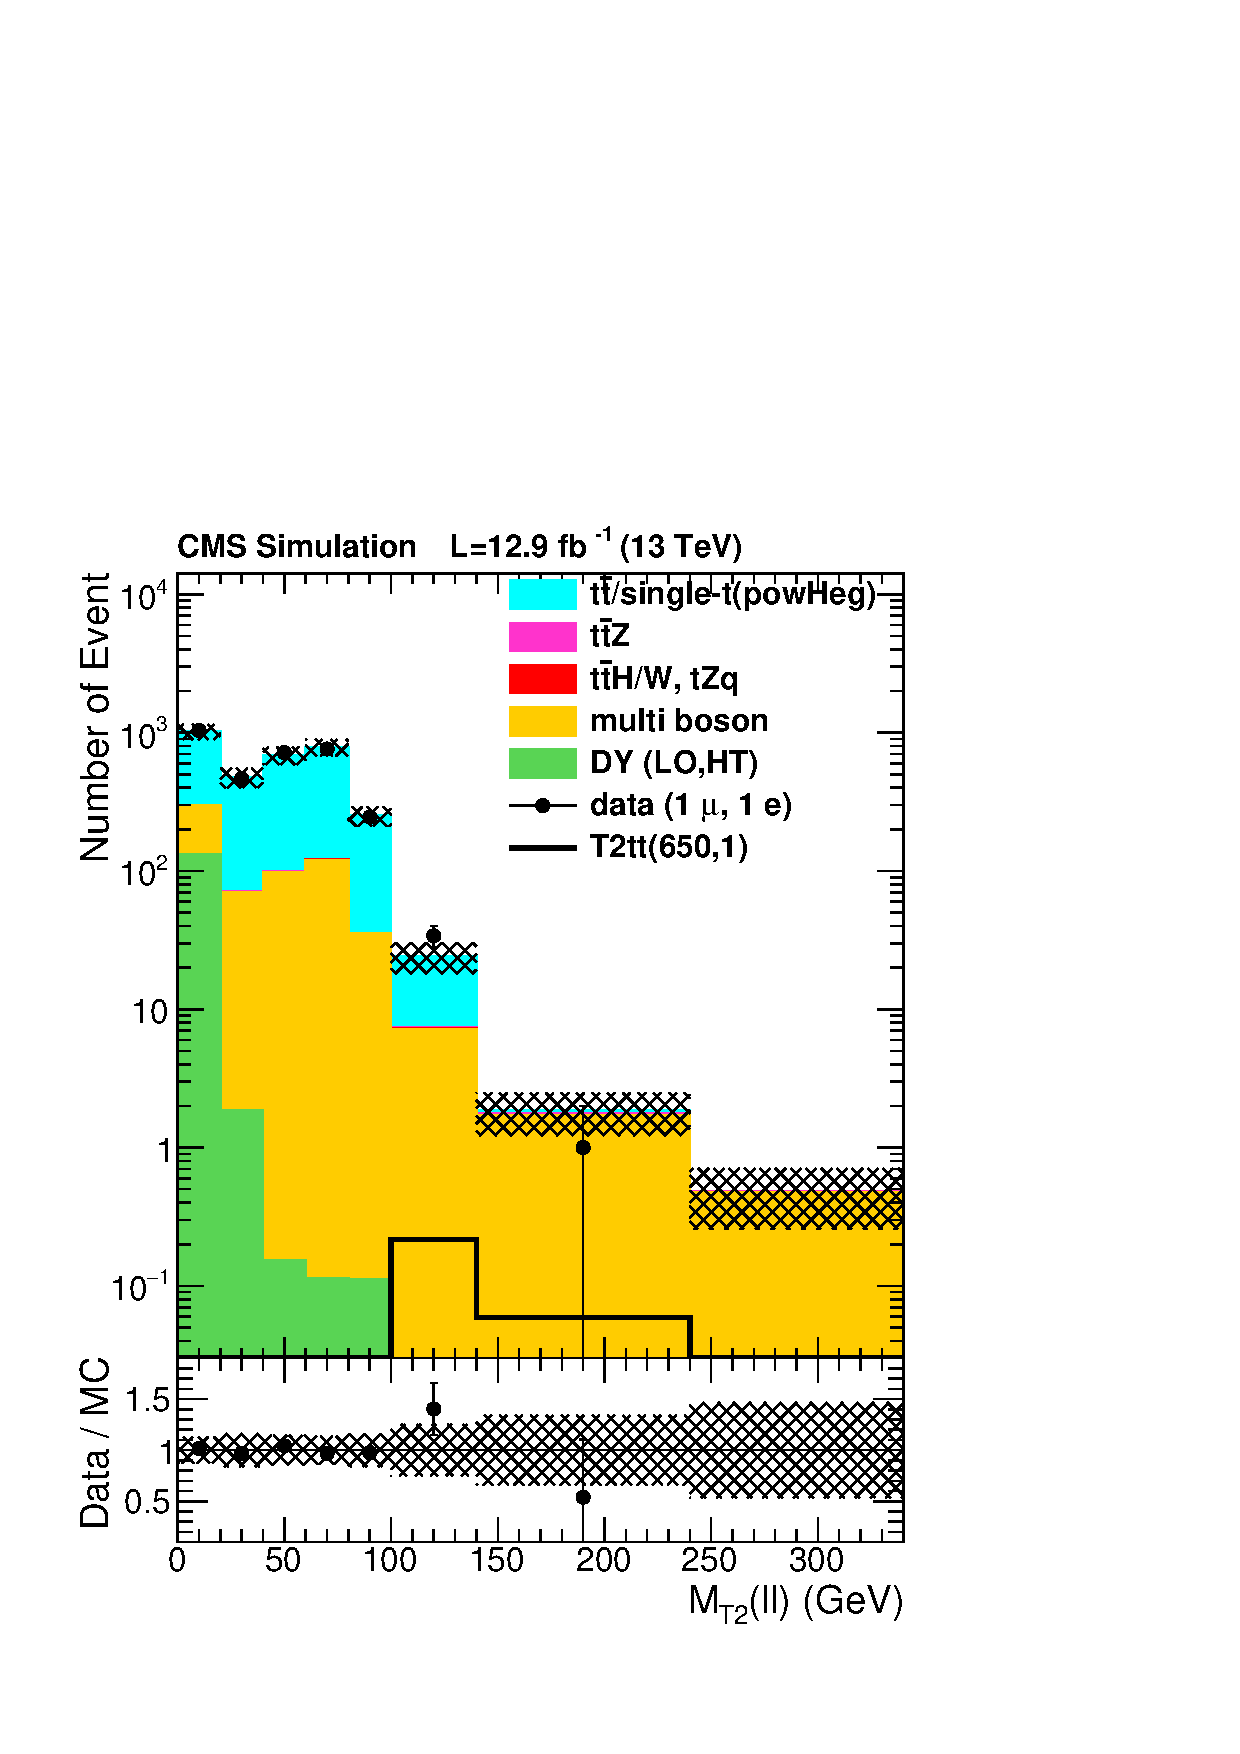
\includegraphics[scale=0.33]{figures/systematicPlots/mue_log_scaled/njet01-btag0-multiIsoWP-looseLeptonVeto-mll20-met80-metSig5/dl_mt2ll.pdf}}
\subfloat[ $\Njets \leq 1$, $\Nbtags\geq1$, high \ETmiss]{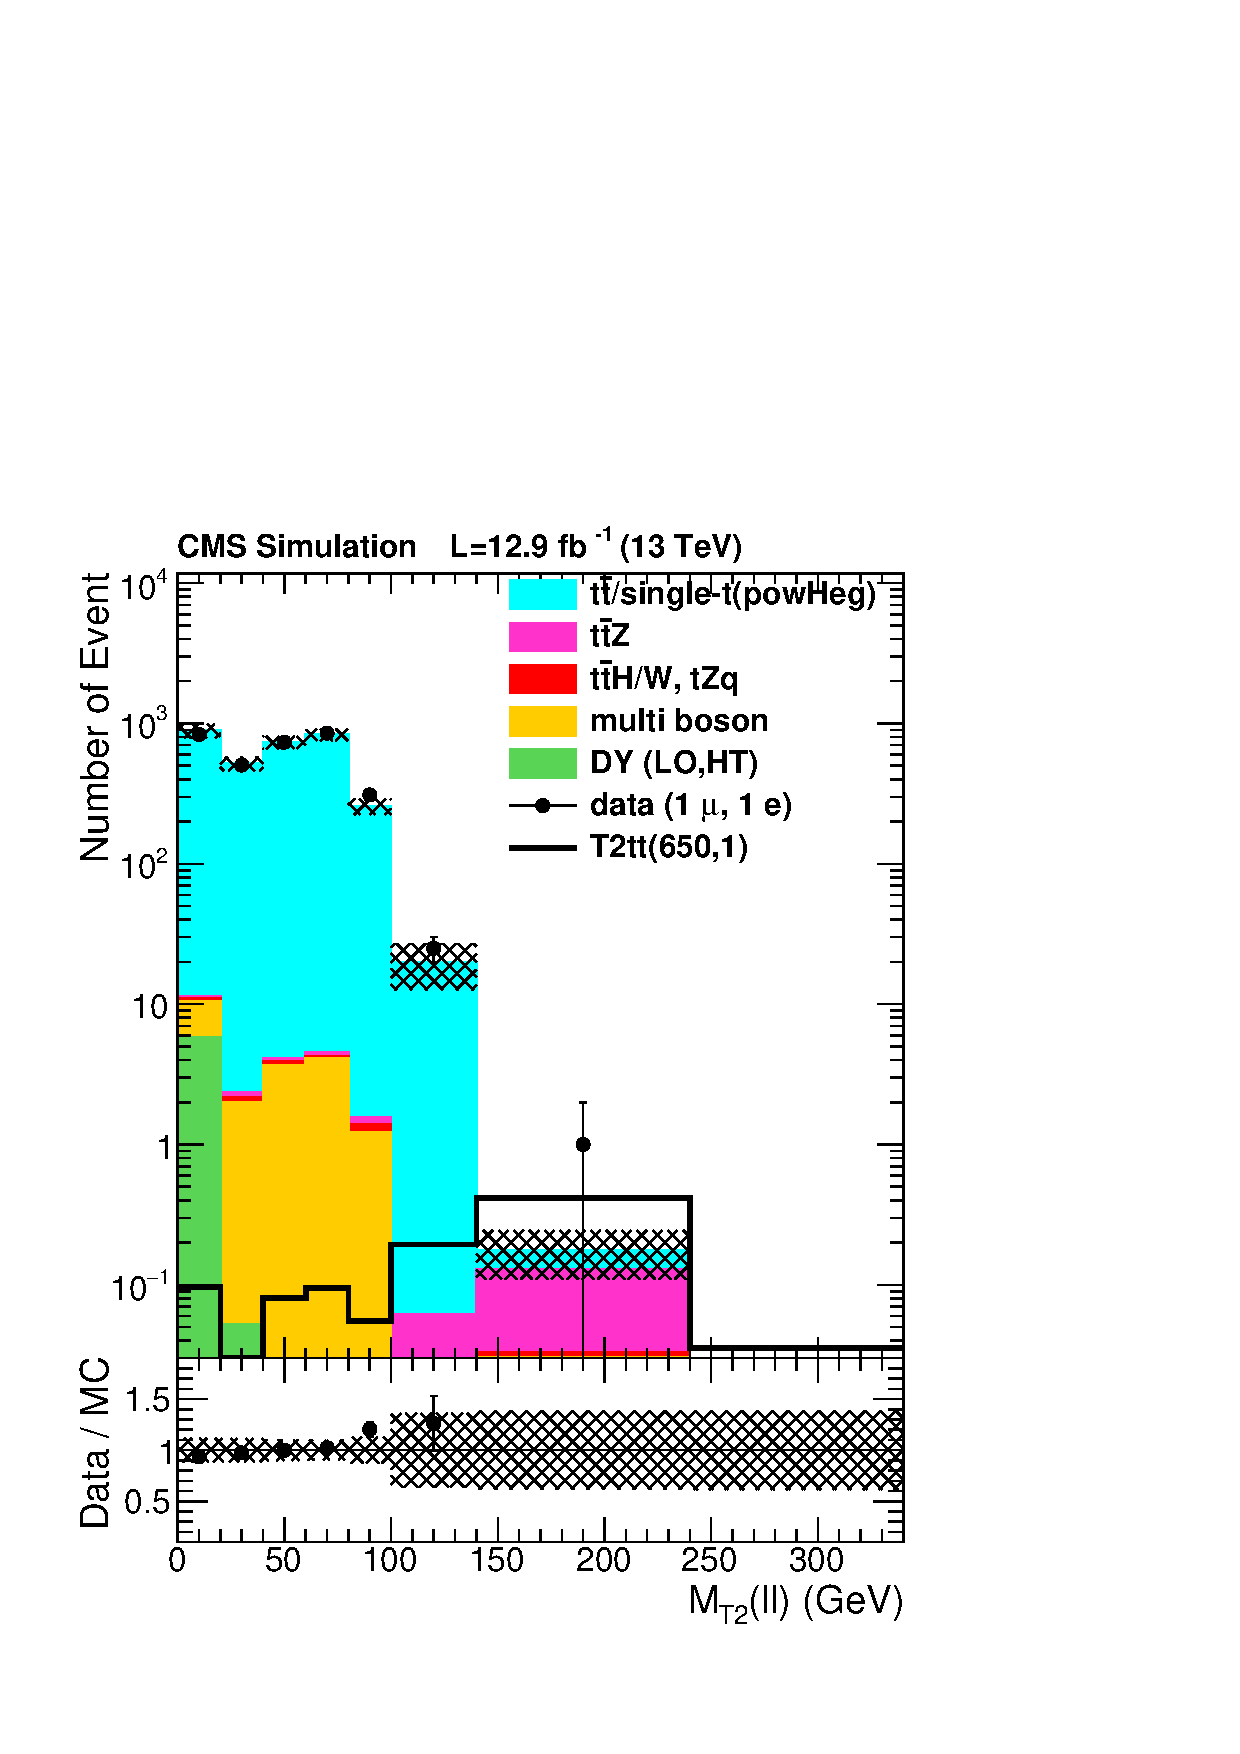
\includegraphics[scale=0.33]{figures/systematicPlots/mue_log_scaled/njet01-btagM-multiIsoWP-looseLeptonVeto-mll20-met80-metSig5/dl_mt2ll.pdf}}
\subfloat[ $\Njets \geq 2$, $\Nbtags=0$, high \ETmiss]{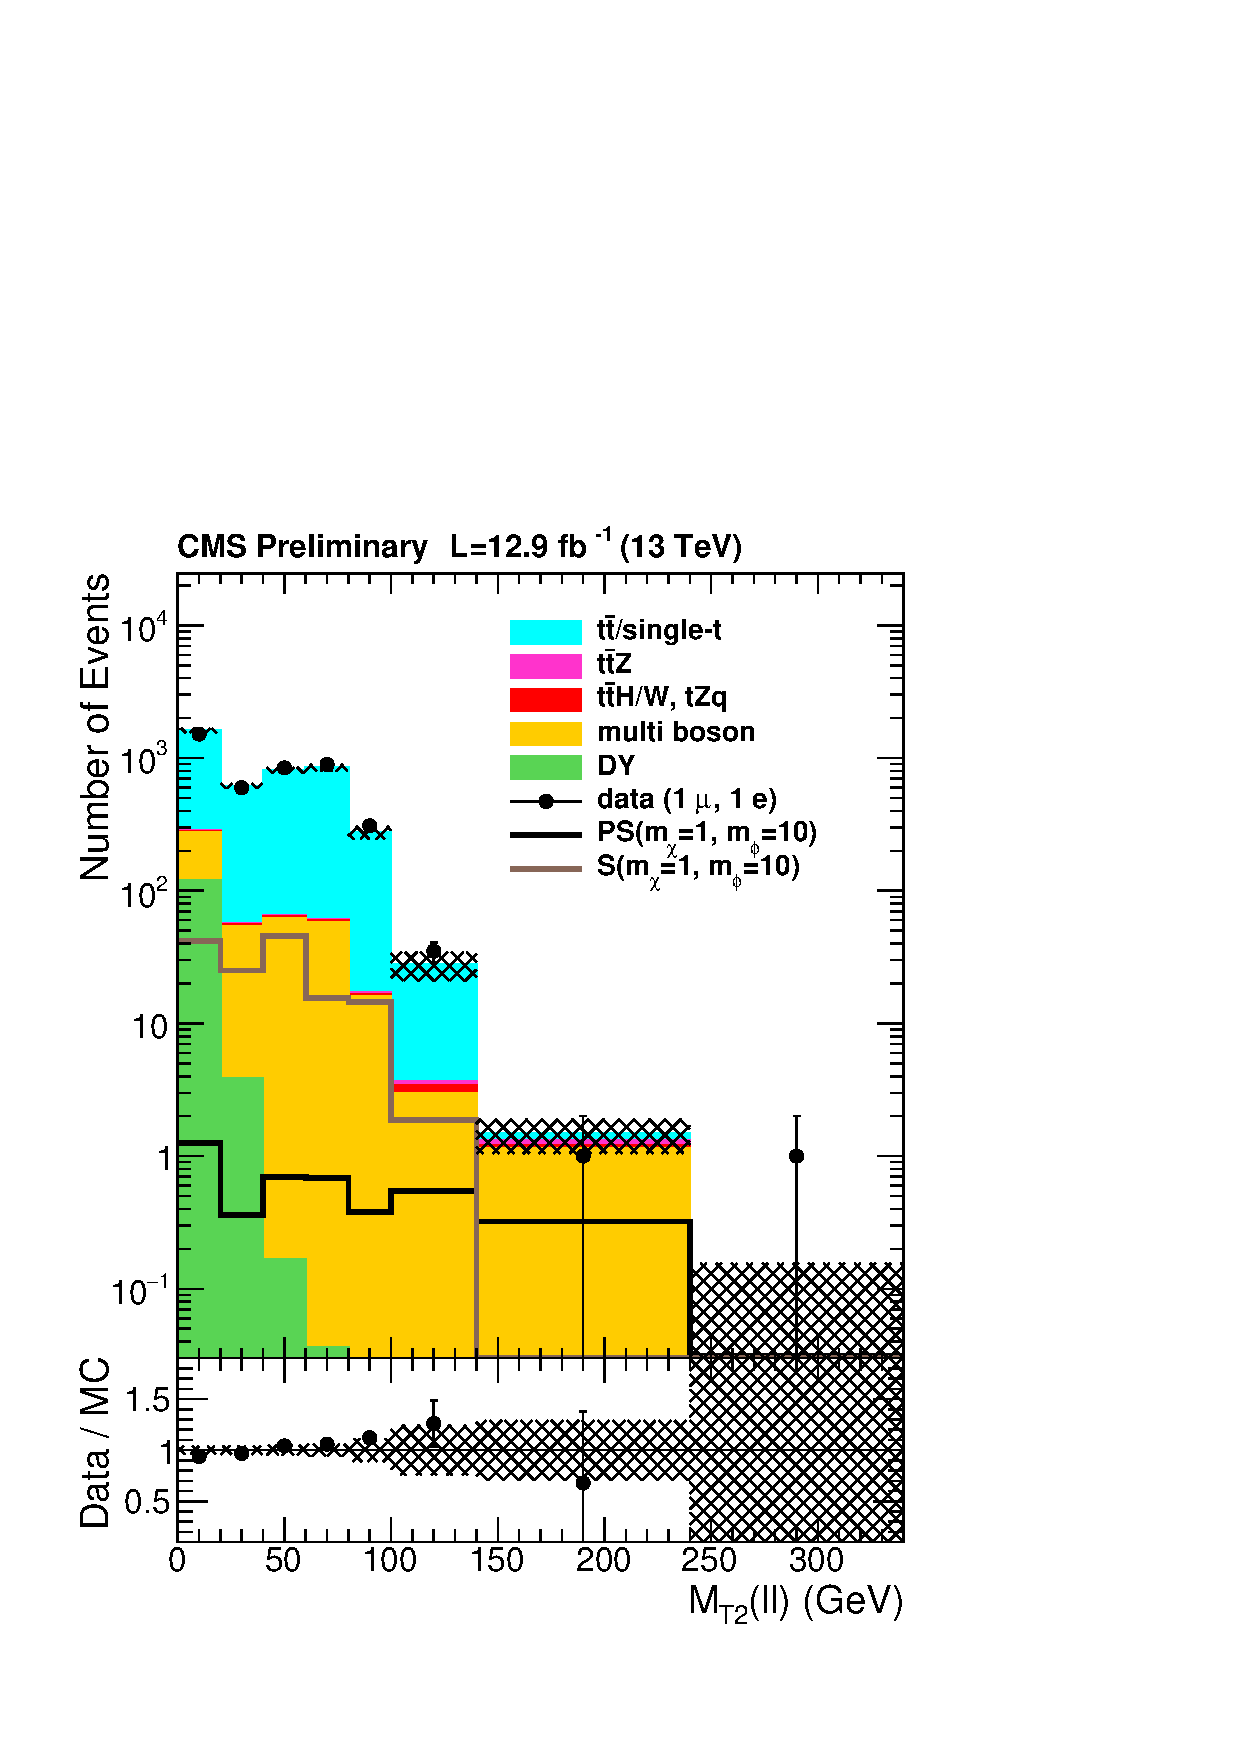
\includegraphics[scale=0.33]{figures/systematicPlots/mue_log_scaled/njet2-btag0-multiIsoWP-looseLeptonVeto-mll20-met80-metSig5/dl_mt2ll.pdf}}\\
\subfloat[ $\Njets \leq 1$, $\Nbtags=0$, low \ETmiss]{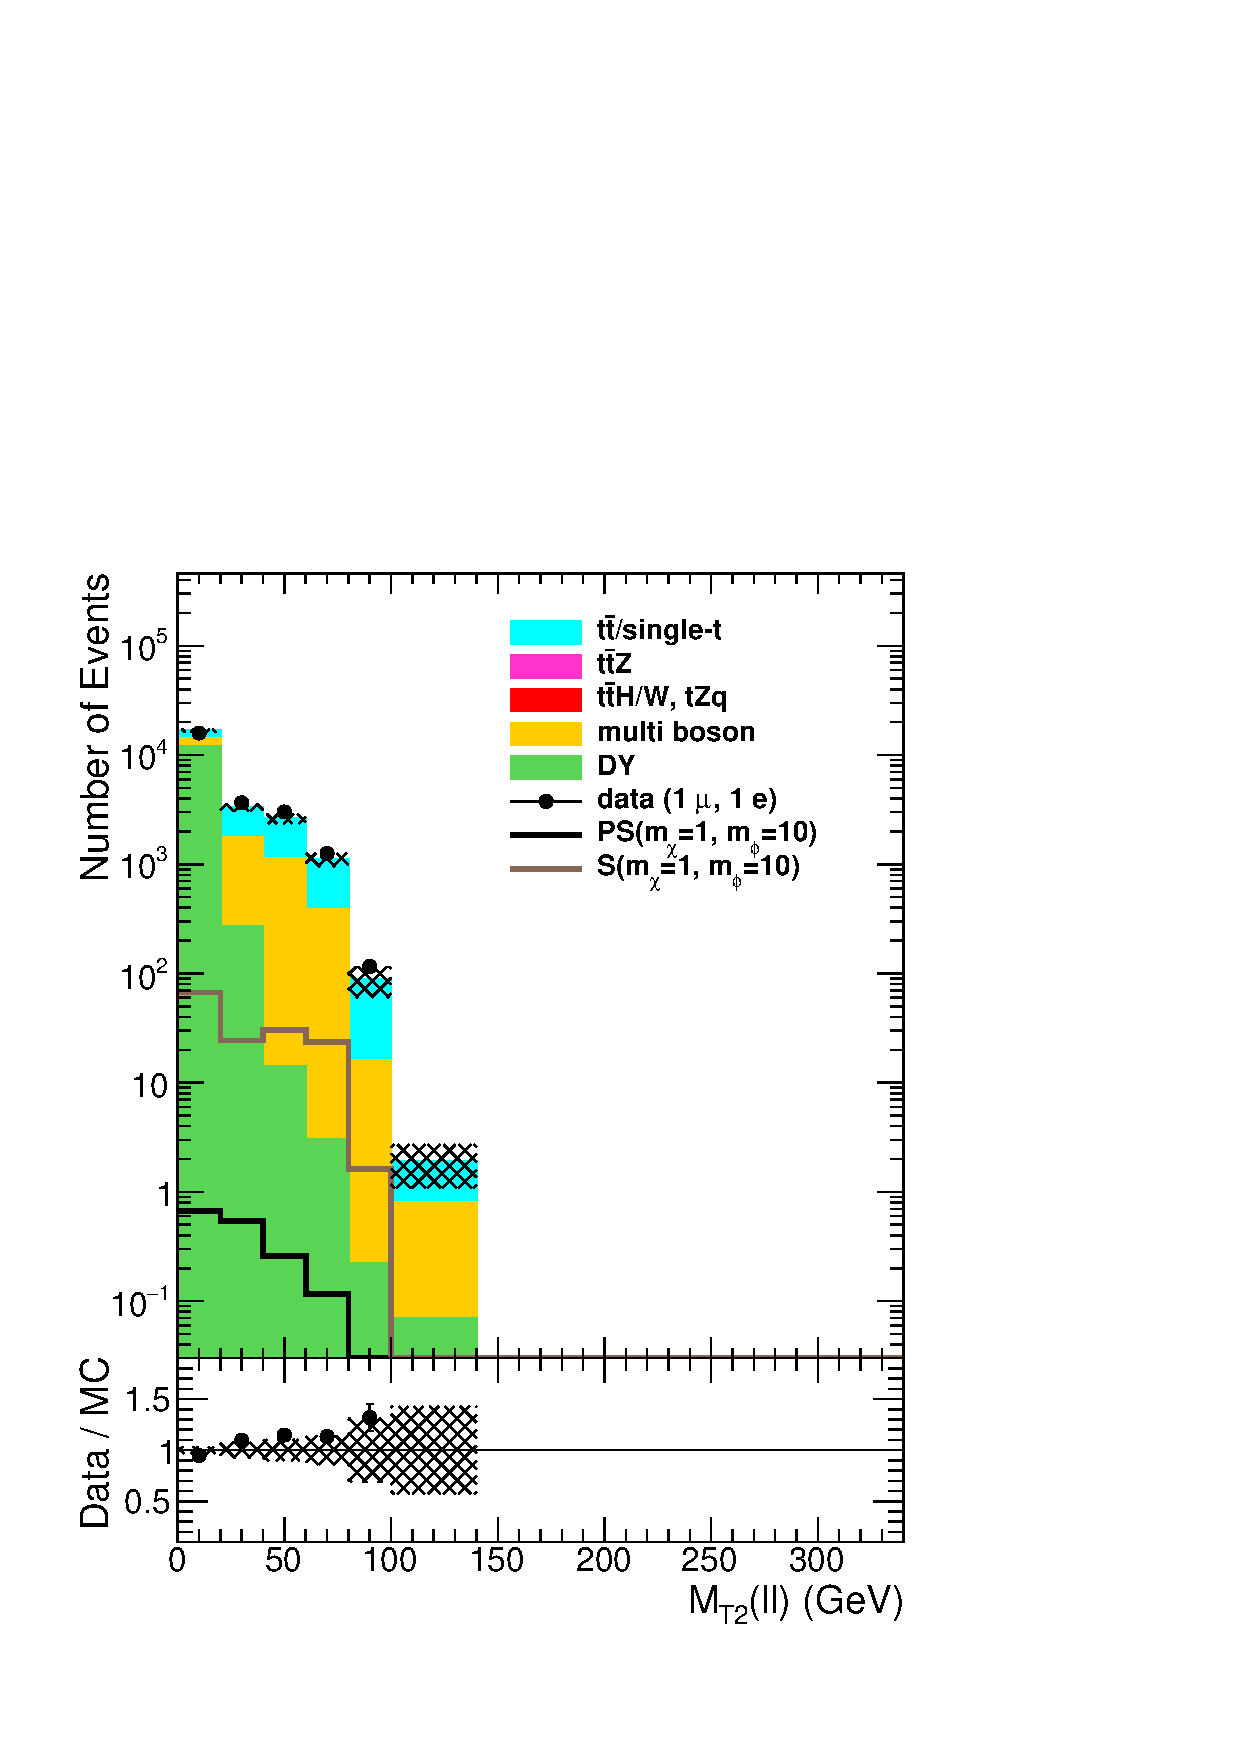
\includegraphics[scale=0.33]{figures/systematicPlots/mue_log_scaled/njet01-btag0-multiIsoWP-looseLeptonVeto-mll20-metInv/dl_mt2ll.pdf}}
\subfloat[ $\Njets \leq 1$, $\Nbtags\geq1$, low \ETmiss]{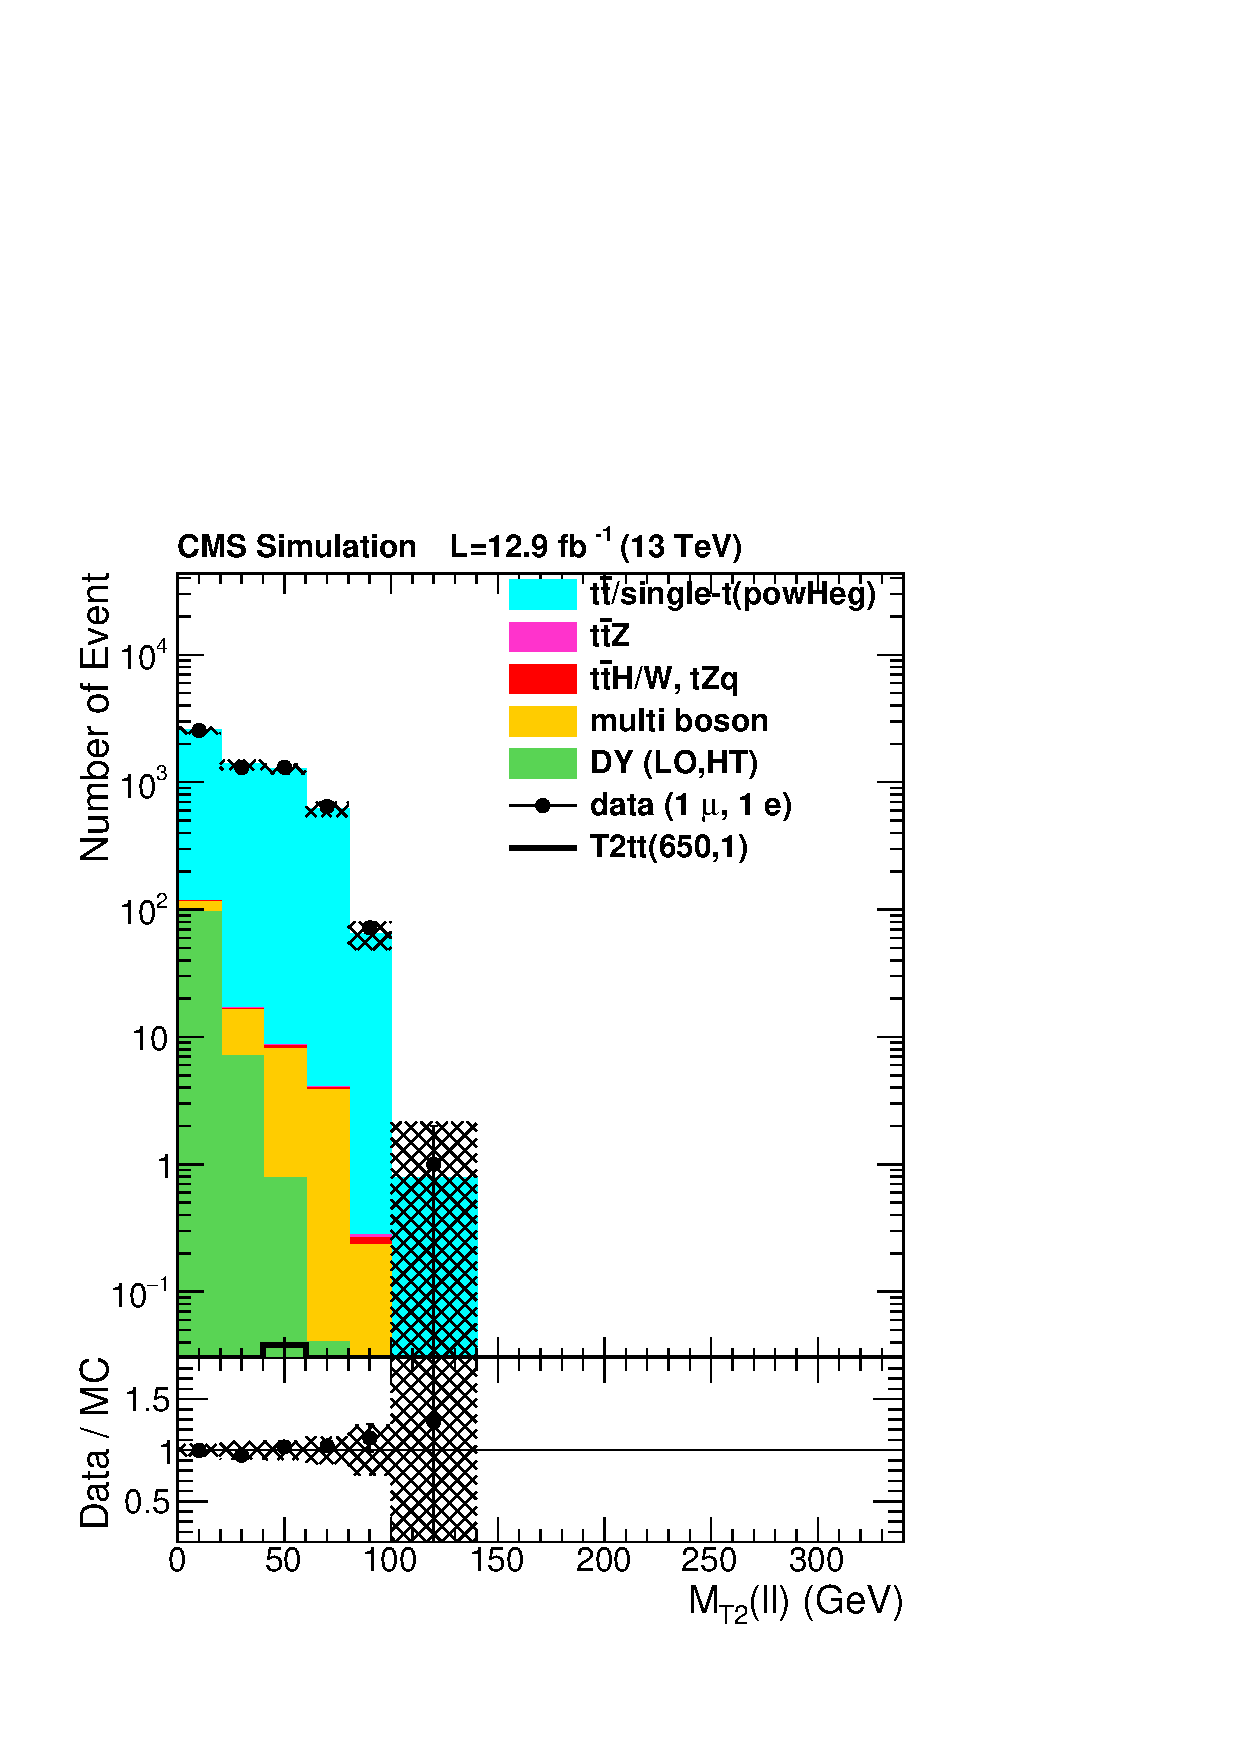
\includegraphics[scale=0.33]{figures/systematicPlots/mue_log_scaled/njet01-btagM-multiIsoWP-looseLeptonVeto-mll20-metInv/dl_mt2ll.pdf}}
\subfloat[ $\Njets \geq 2$, $\Nbtags=0$, low \ETmiss]{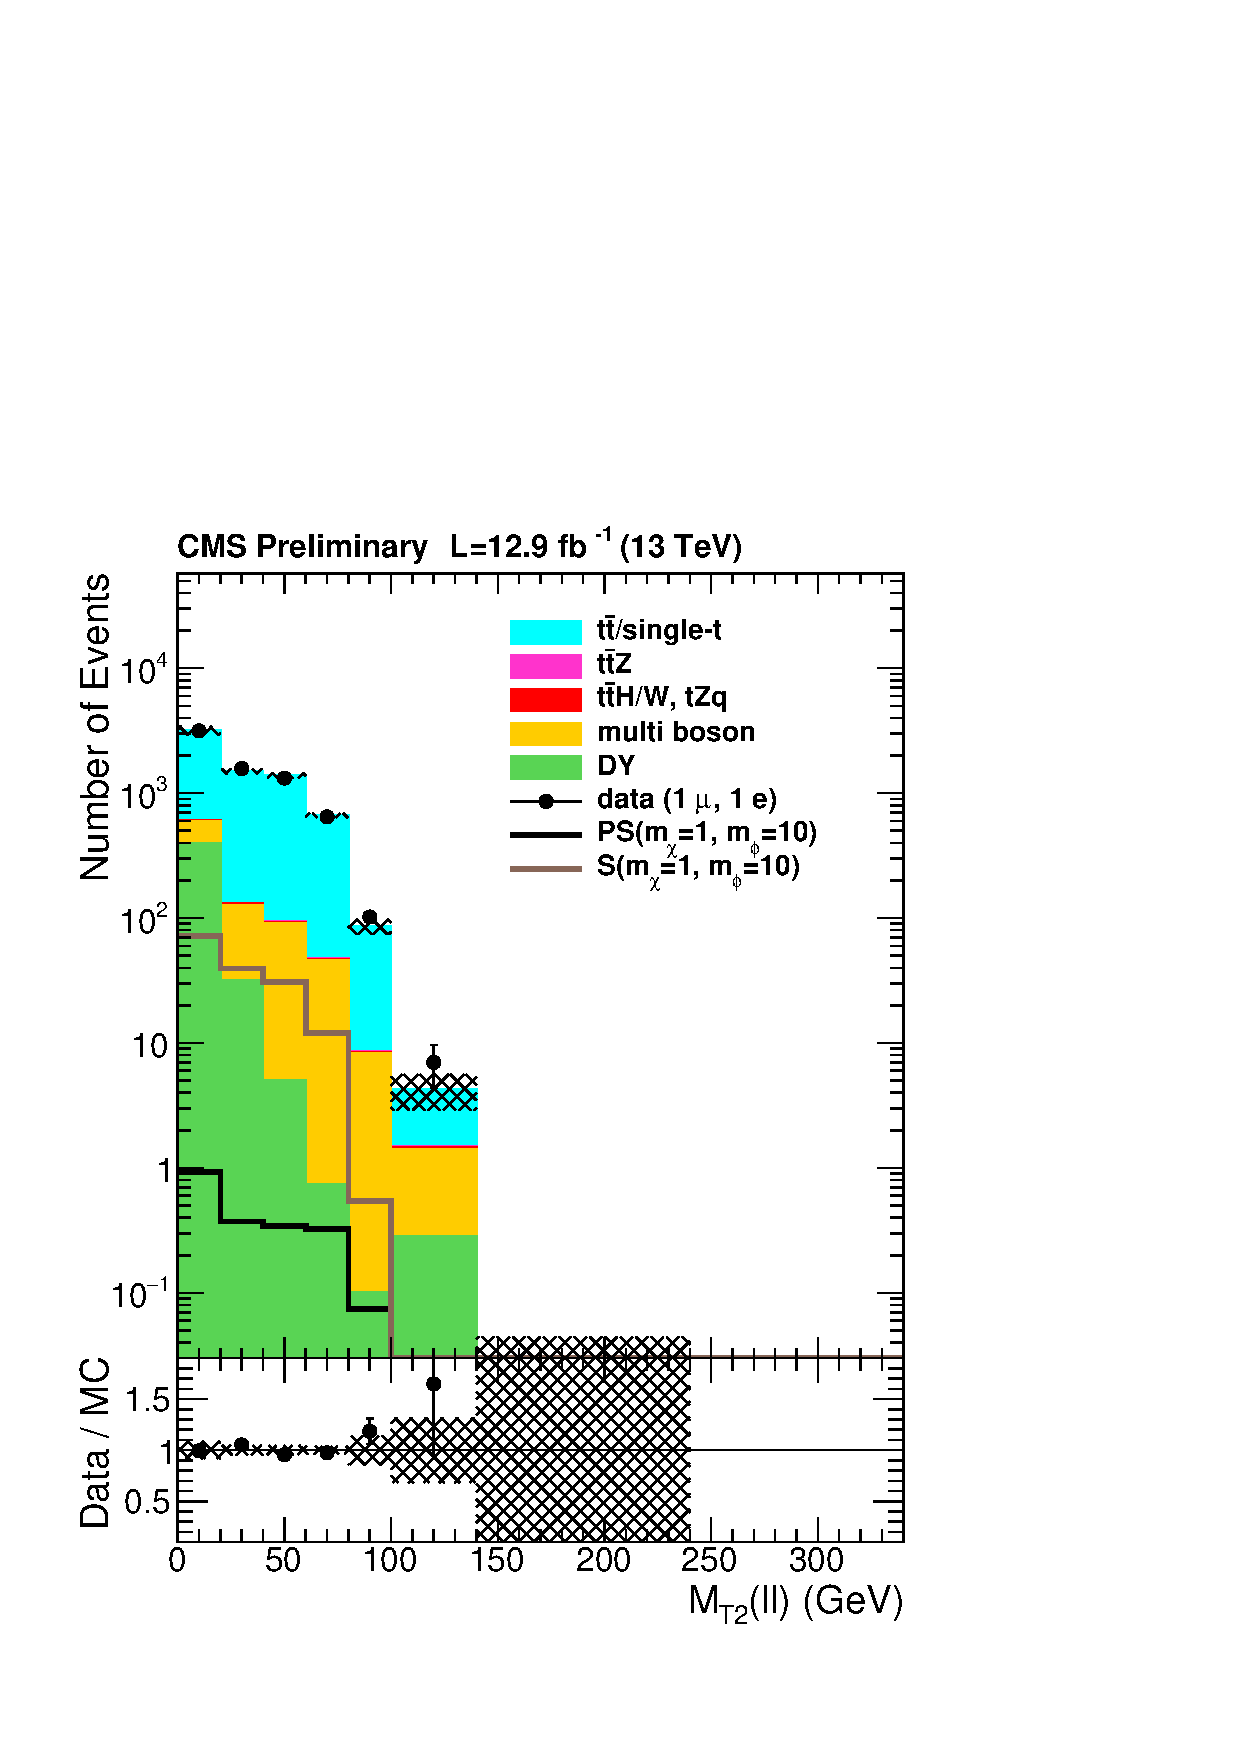
\includegraphics[scale=0.33]{figures/systematicPlots/mue_log_scaled/njet2-btag0-multiIsoWP-looseLeptonVeto-mll20-metInv/dl_mt2ll.pdf}}\\
\subfloat[ $\Njets \geq 2$, $\Nbtags\geq1$, low \ETmiss]{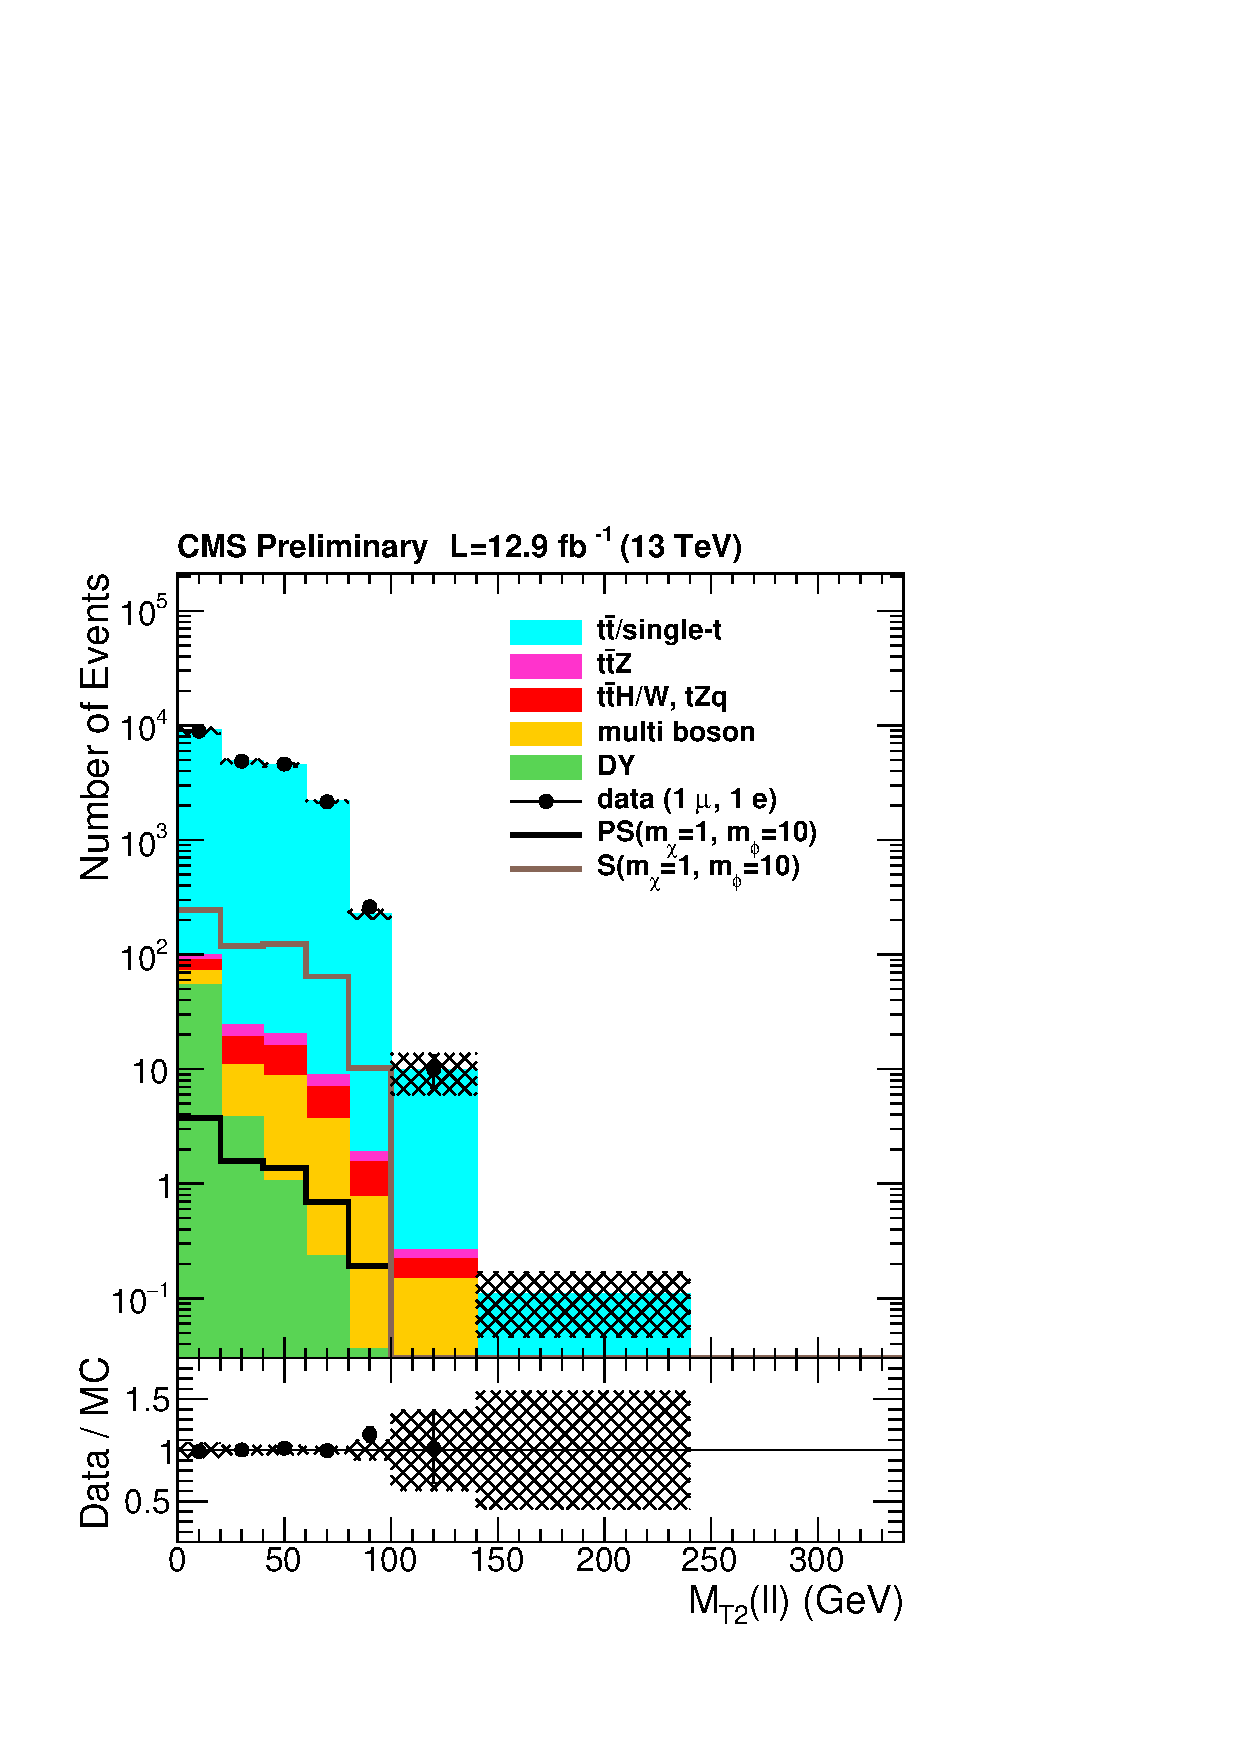
\includegraphics[scale=0.33]{figures/systematicPlots/mue_log_scaled/njet2-btagM-multiIsoWP-looseLeptonVeto-mll20-metInv/dl_mt2ll.pdf}}
\caption{\mtll distributions in opposite flavor control regions enriched by $t\bar{t}$ events. MC yields are normalized to data using the yields at $\mtll<100$ \GeV.  }
\label{fig:ttBar_controlPlots}
\end{figure}

Going beyond the check of the rate of events with large jet mismeasurements in Sec.~\ref{sec:met_tail}, we next check the shape of the \mtll distribution in \ttbar due to \ETmiss mismeasurements and any other potential sources.
In order to remove contamination from DY we require different flavor leptons. 
Figure~\ref{fig:ttBar_controlPlots}  shows the \mtll distribution compared to simulation for various selections. Comparisons are performed in high \ETmiss regions
that are defined by $\ETmiss>80$ \GeV and $\metSig>5$ for different jet and b-tag multiplicities. Of course we omit the signal region by skipping the case $\Njets \geq 2$, $\Nbtags\geq1$.
In the low \ETmiss signal regions given by $\ETmiss<80$ \GeV that case can be included as well. 

We observe a good agreement between \mtll shape from data and simulation over three orders of magnitude change of yields per bin. 
The uncertainty due to experimental effects is shown with a hatched band.

\subsubsection{Summary of \texorpdfstring{\ttbar}{ttbar} background estimation.}

Based on these checks in the control regions we proceed with using MC simulation to predict the top background contribution in the signal regions and we use data events in $\mtll <100$~\GeV for the absolute normalization. 
The normalization is done in each of the channels and yields the following scale factors: $0.867\pm0.010$ in the $\mu\mu$ channel, $0.892\pm0.017$ in the $ee$ channel and $0.861 \pm 0.009$ for $e\mu$ events.
In this way, the experimental uncertainties affecting the overall normalization are largely reduced.
Figure~\ref{fig:ttBar_controlPlots}f shows the side-band with zero b-tagged jets that we use to assign a systematic uncertainty on the \ttbar shape. 
We find 7 events satisfying $\mtll>100$~\GeV and 4.6 events predicted. Despite the fact that statistical uncertainties are large, we apply an uncertainty on the \mtll yield of 50\% for $\mtll<240$~\GeV and 100\% above that threshold.

%Finally, we checked that a veto on hadronically decaying $tau$ leptons does not change the sensitivity of the analysis. 


  \subsection{Estimation of Drell-Yan and diboson backgrounds}
\label{sec:DY_diboson}

The background from Drell-Yan (DY) events is strongly reduced by our event selection which applies several cuts on \met-related variables.
In this section, we discuss these cuts and the properties of the DY background in more detail using a  
control region defined by a 0 b-jet requirement and an on-Z requirement defined by $|m_{ll} - m_Z| < 15$ GeV.

Figure~\ref{fig:DY} shows the distributions of \metSig and \mtll  for same-flavour ($ee$/$\mu\mu$) events in this control region, 
before applying the $\metSig>5$ cut. Because \met in DY events typically arises from jet mismeasurements, large \met will be countered by large \HT, and hence
the \metSig distribution peaks below 5 for the DY background.  
Backgrounds with genuine \ETmiss (and the signal) are typically concentrated at higher~\metSig.

When \met originates from jet mismeasurements, it is also likely to align with one of the jets, which is exploited by the cuts on the $\cos{\Delta\phi(\met, \text{jet})}$ variables that are shown in Fig.~\ref{fig:DY_afterMetSig} for the two leading jets and after applying the $\metSig>5$ cut. 
It can readily be seen that this selection is dominated by a mixture of DY and multiboson contributions that we now separate. 
In DY events, the \ETmiss will be dominated by mismeasurement of jets. 
If we therefore veto events where one of the two leading jets is aligned with \ETmiss according to $\cos{\Delta\phi(\met, \text{leading jet})} > 0.8$ or $\cos{\Delta\phi(\met, \text{2nd leading jet})} > \cos{0.25}=0.96$, 
we can define a region where DY is pure. 
The reason for the relatively small angular separation of \ETmiss w.r.t to the sub-leading jet that it should select events with
drastic mismeasurements. Indeed, it can happen that the leading generated jet looses enough energy such that it is reconstructed as the subleading jet. 
In such cases, \ETmiss is typically aligned with the sub-leading jet to within half the jet clustering distance.

In Fig.~\ref{fig:DY_dPhiInv}a, we show the \mtll distribution in this selection. The purity of DY is 84\%. 
Subtracting from data any residual electroweak contributions according to
\begin{equation}
R = \frac{n_\text{data}-n_\text{residual}}{n_\text{DY}},
\end{equation} 
we find a scale factor for DY of $1.30\pm 0.12$.

In order to justify that the scale factor is applied inclusively to the sample, we note that the \Nbtags shape is consistent with a flat scaling as shown in Fig.~\ref{fig:DY_nbtag_validation}a.
In Fig.~\ref{fig:DY_nbtag_validation}b we show the \Nbtags multiplicity after removing \mtll, \ETmiss, \metSig and $\Delta\phi$ requirements. This demonstrates the quality of \Nbtags modeling in simulated DY events. 

\begin{figure}[!hbtp]
\centering
\subfloat[\metSig]{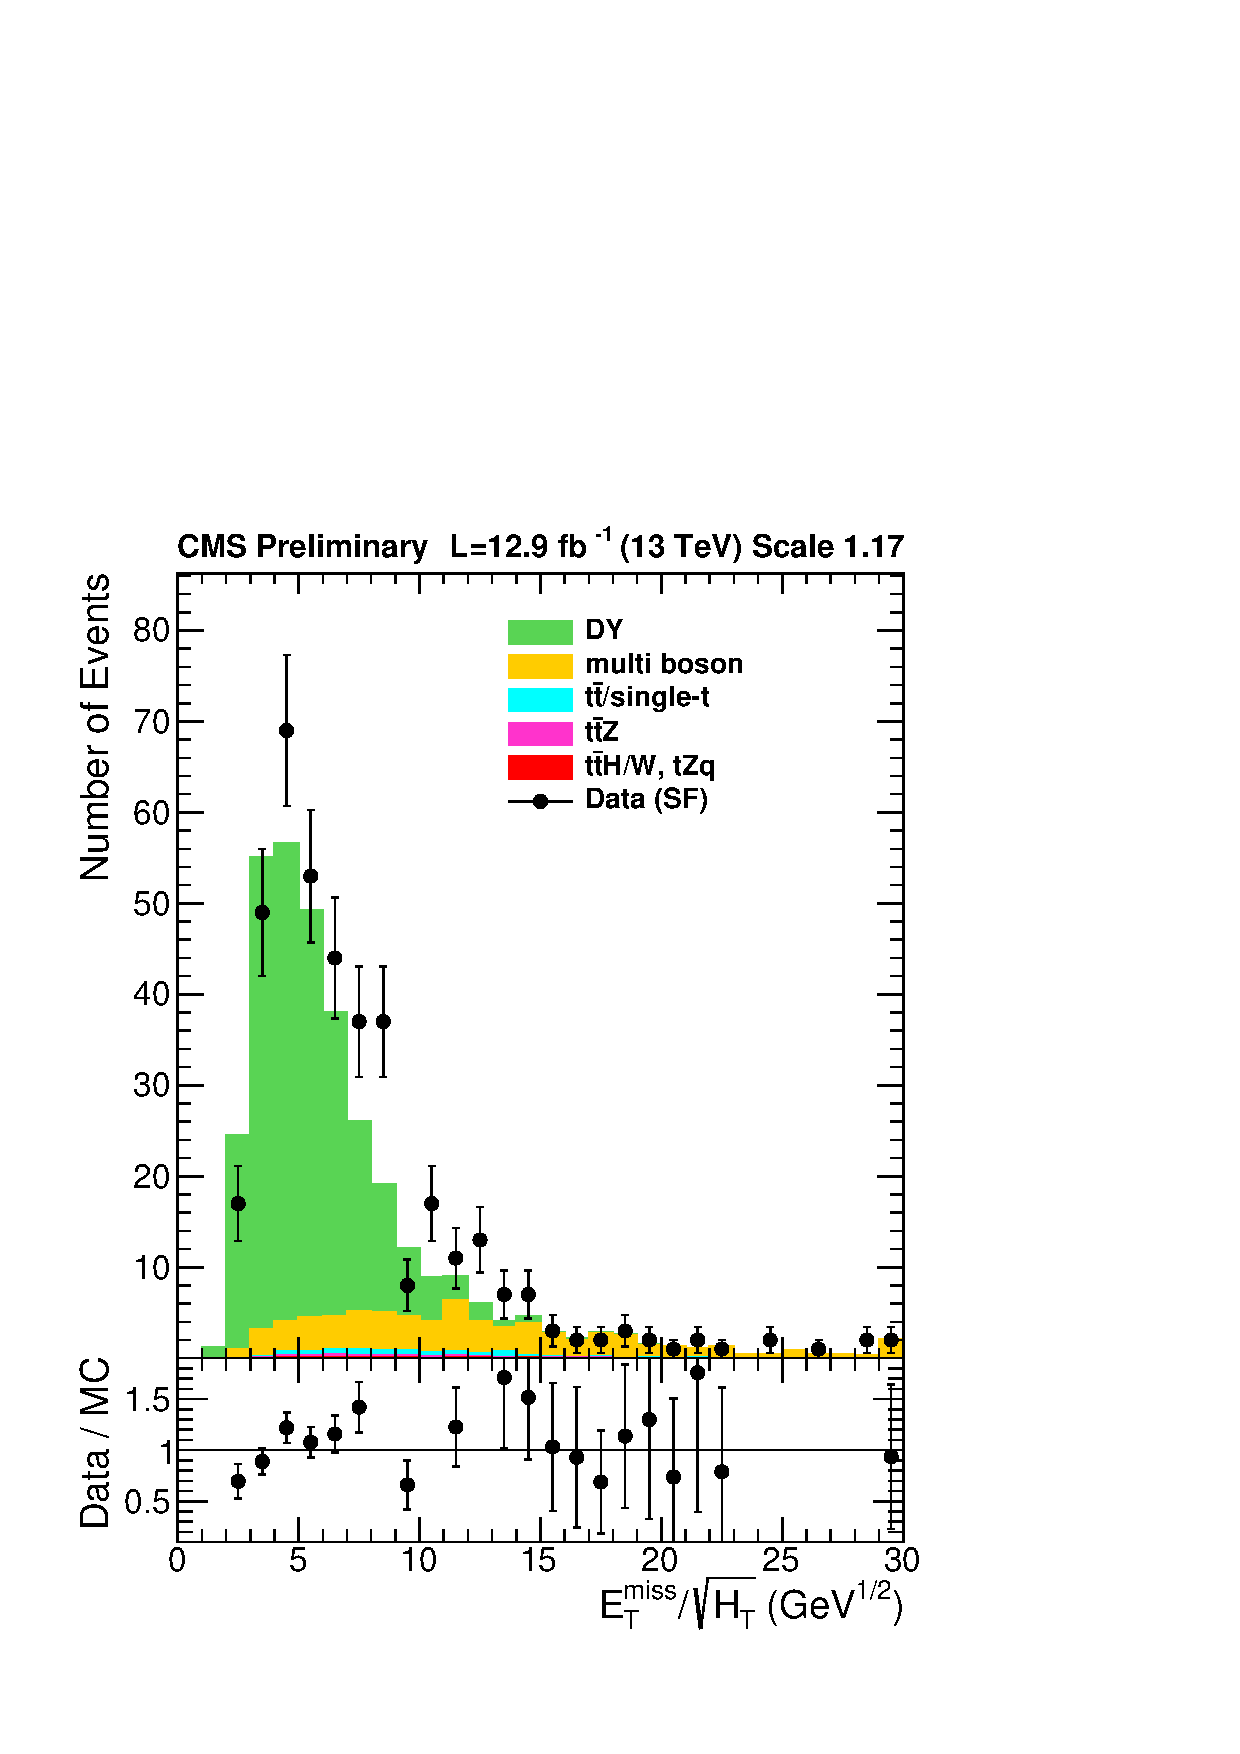
\includegraphics[width=0.45\textwidth]{figures/analysisPlots/SF/njet2-btag0-multiIsoWP-looseLeptonVeto-mll20-onZ-met80-mt2ll100/metSig.pdf}}
\subfloat[\mtll]{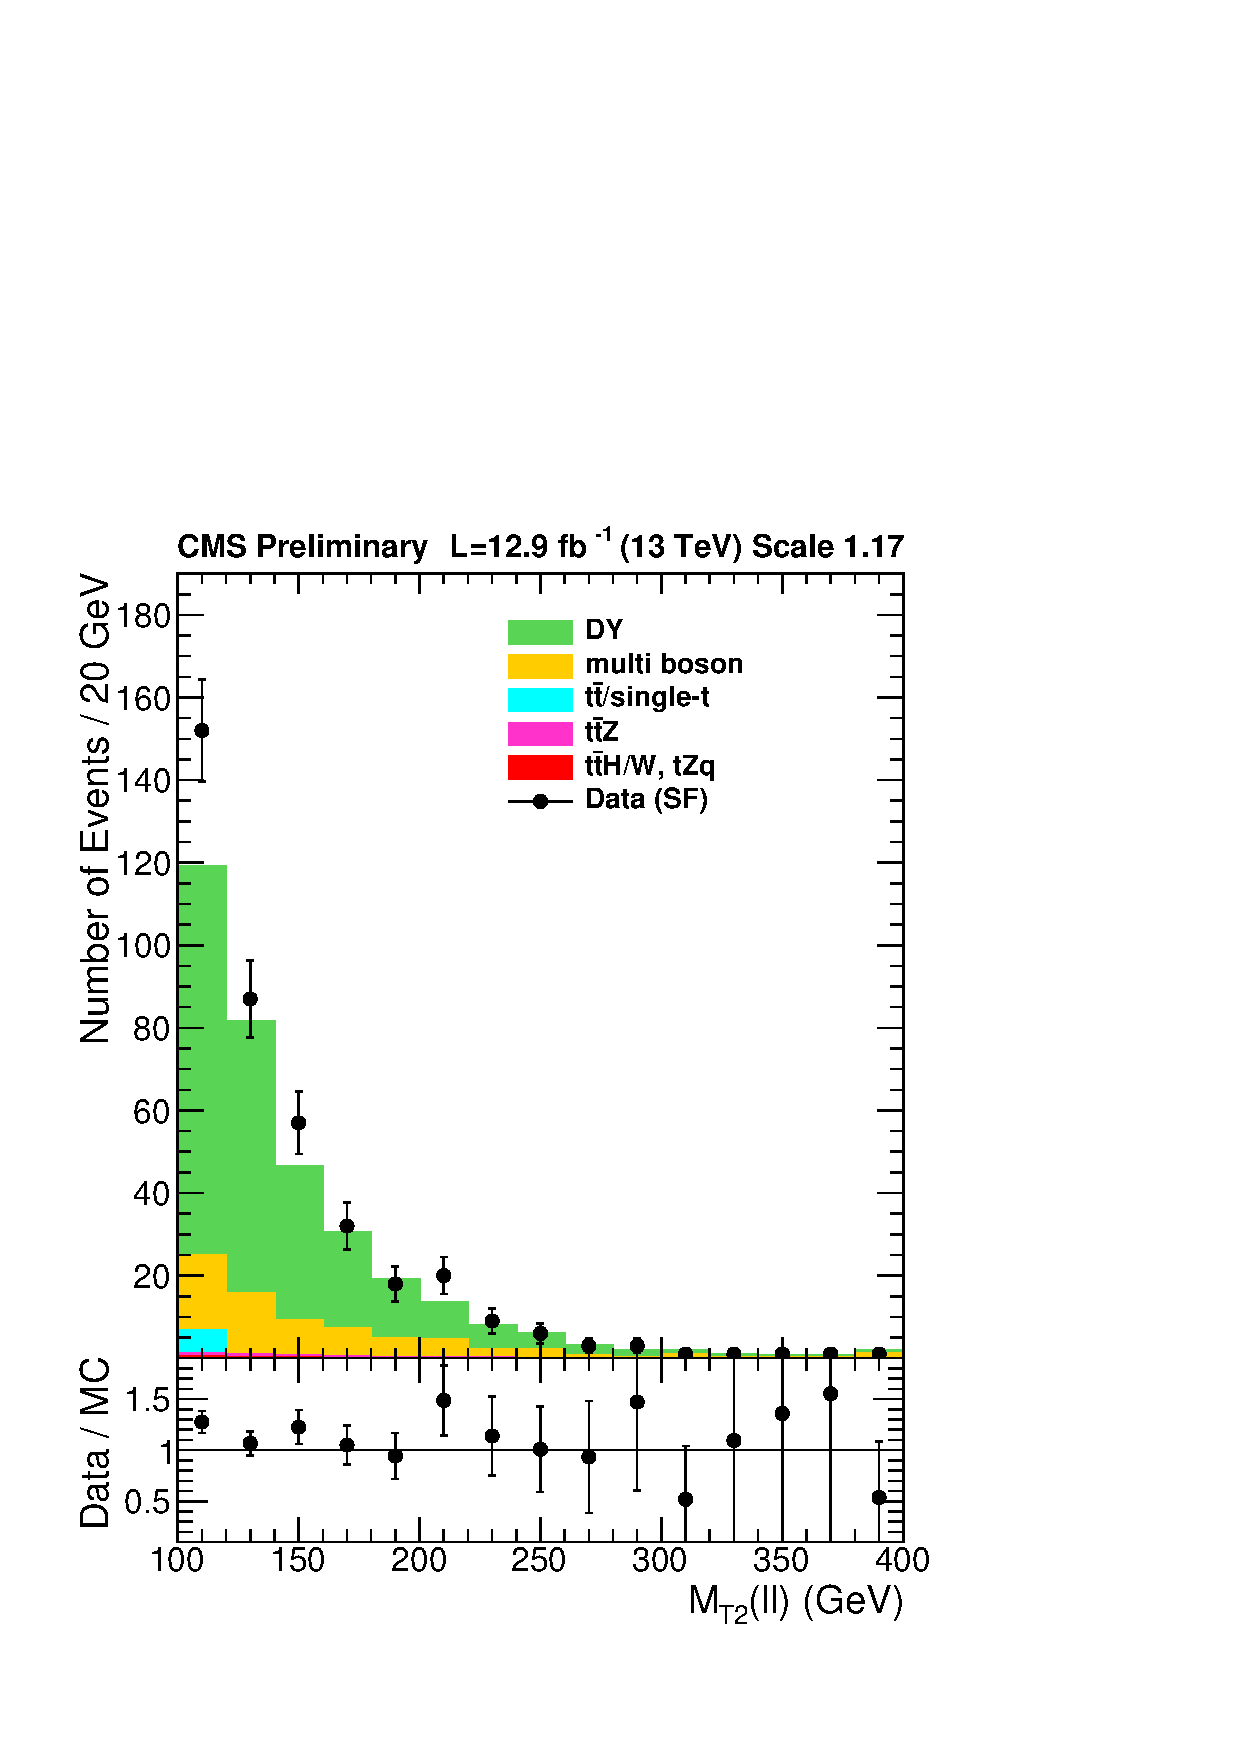
\includegraphics[width=0.45\textwidth]{figures/analysisPlots/SF/njet2-btag0-multiIsoWP-looseLeptonVeto-mll20-onZ-met80-mt2ll100/dl_mt2ll.pdf}} \\
%   \subfloat[$\cos{\Delta\phi(\met, \text{leading jet})}$]{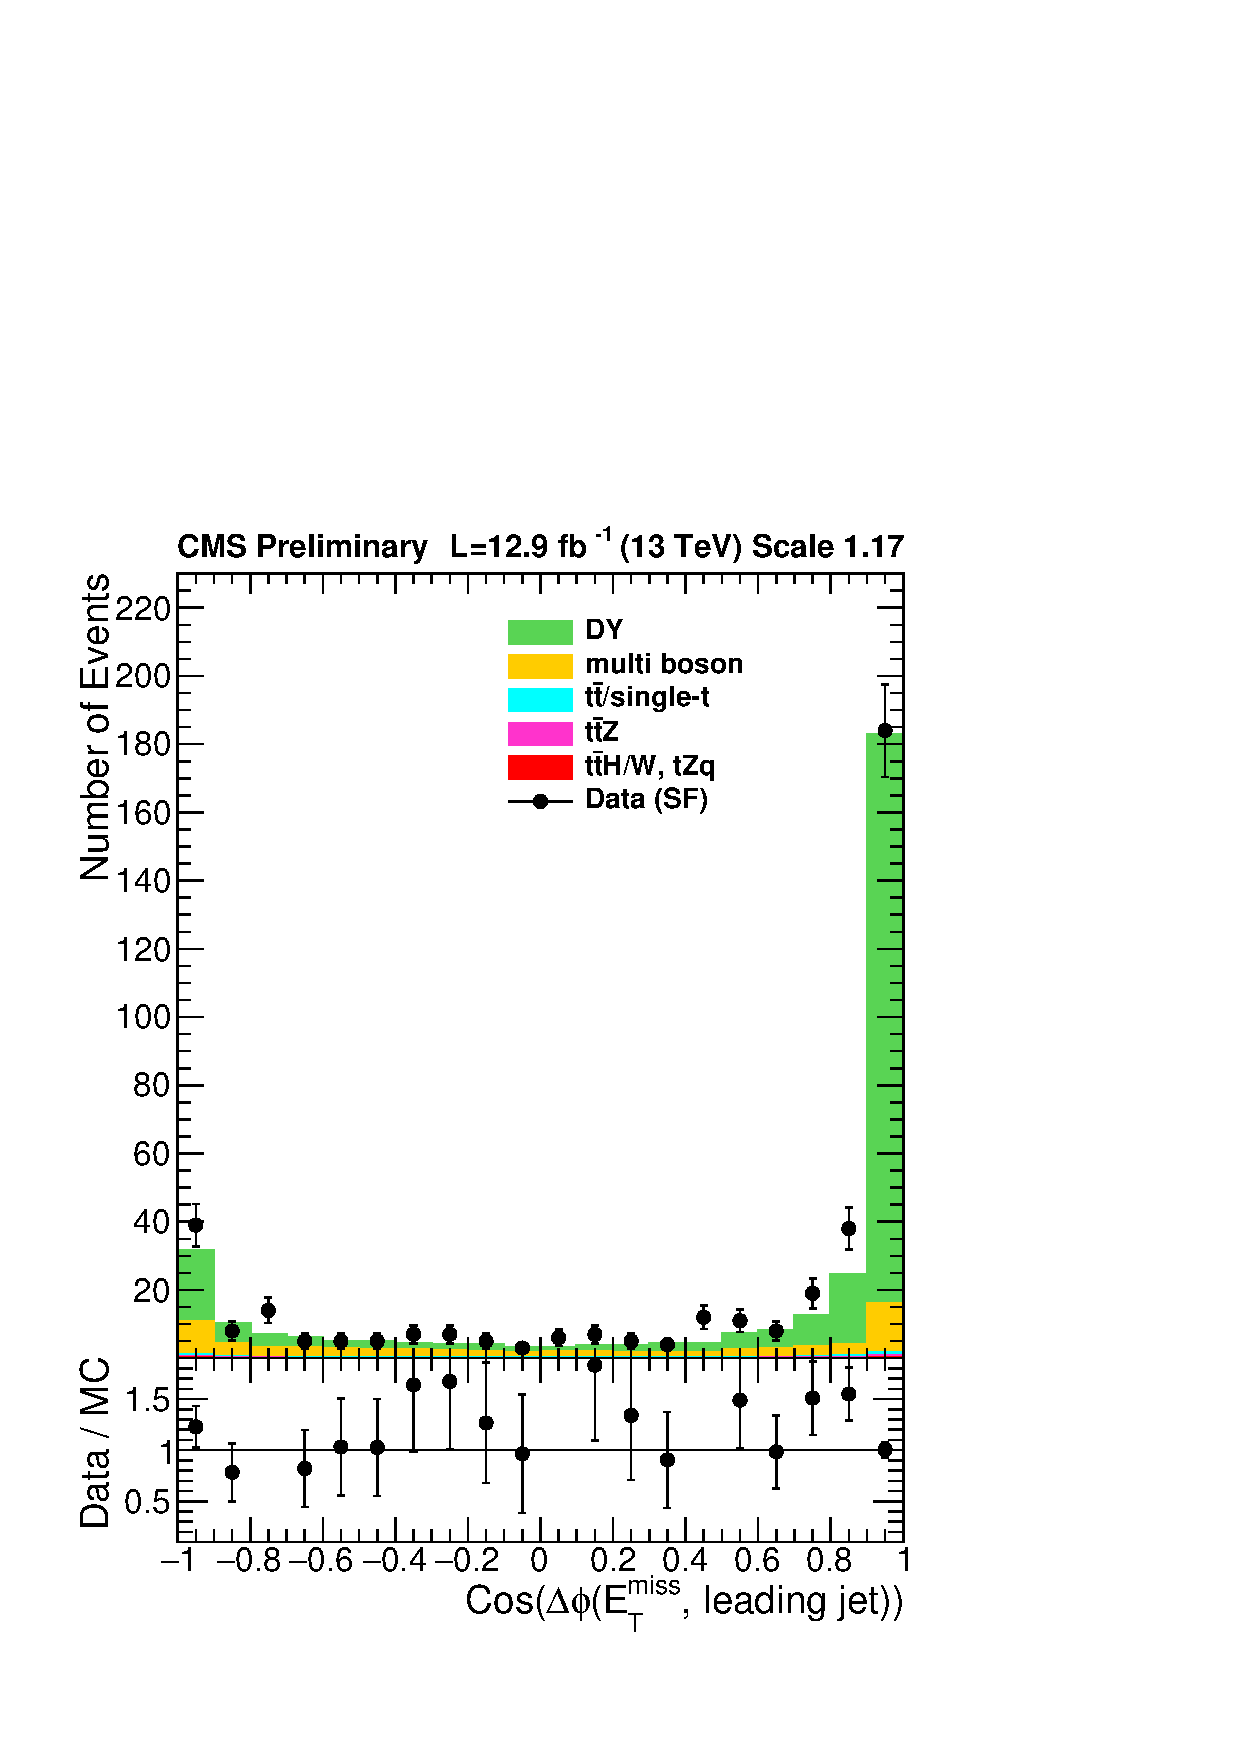
\includegraphics[width=0.45\textwidth]{figures/analysisPlots/SF/njet2-btag0-multiIsoWP-looseLeptonVeto-mll20-onZ-met80-mt2ll100/cosMetJet1phi_smallBinning.pdf}}
%   \subfloat[$\cos{\Delta\phi(\met, \text{2nd leading jet})}$]{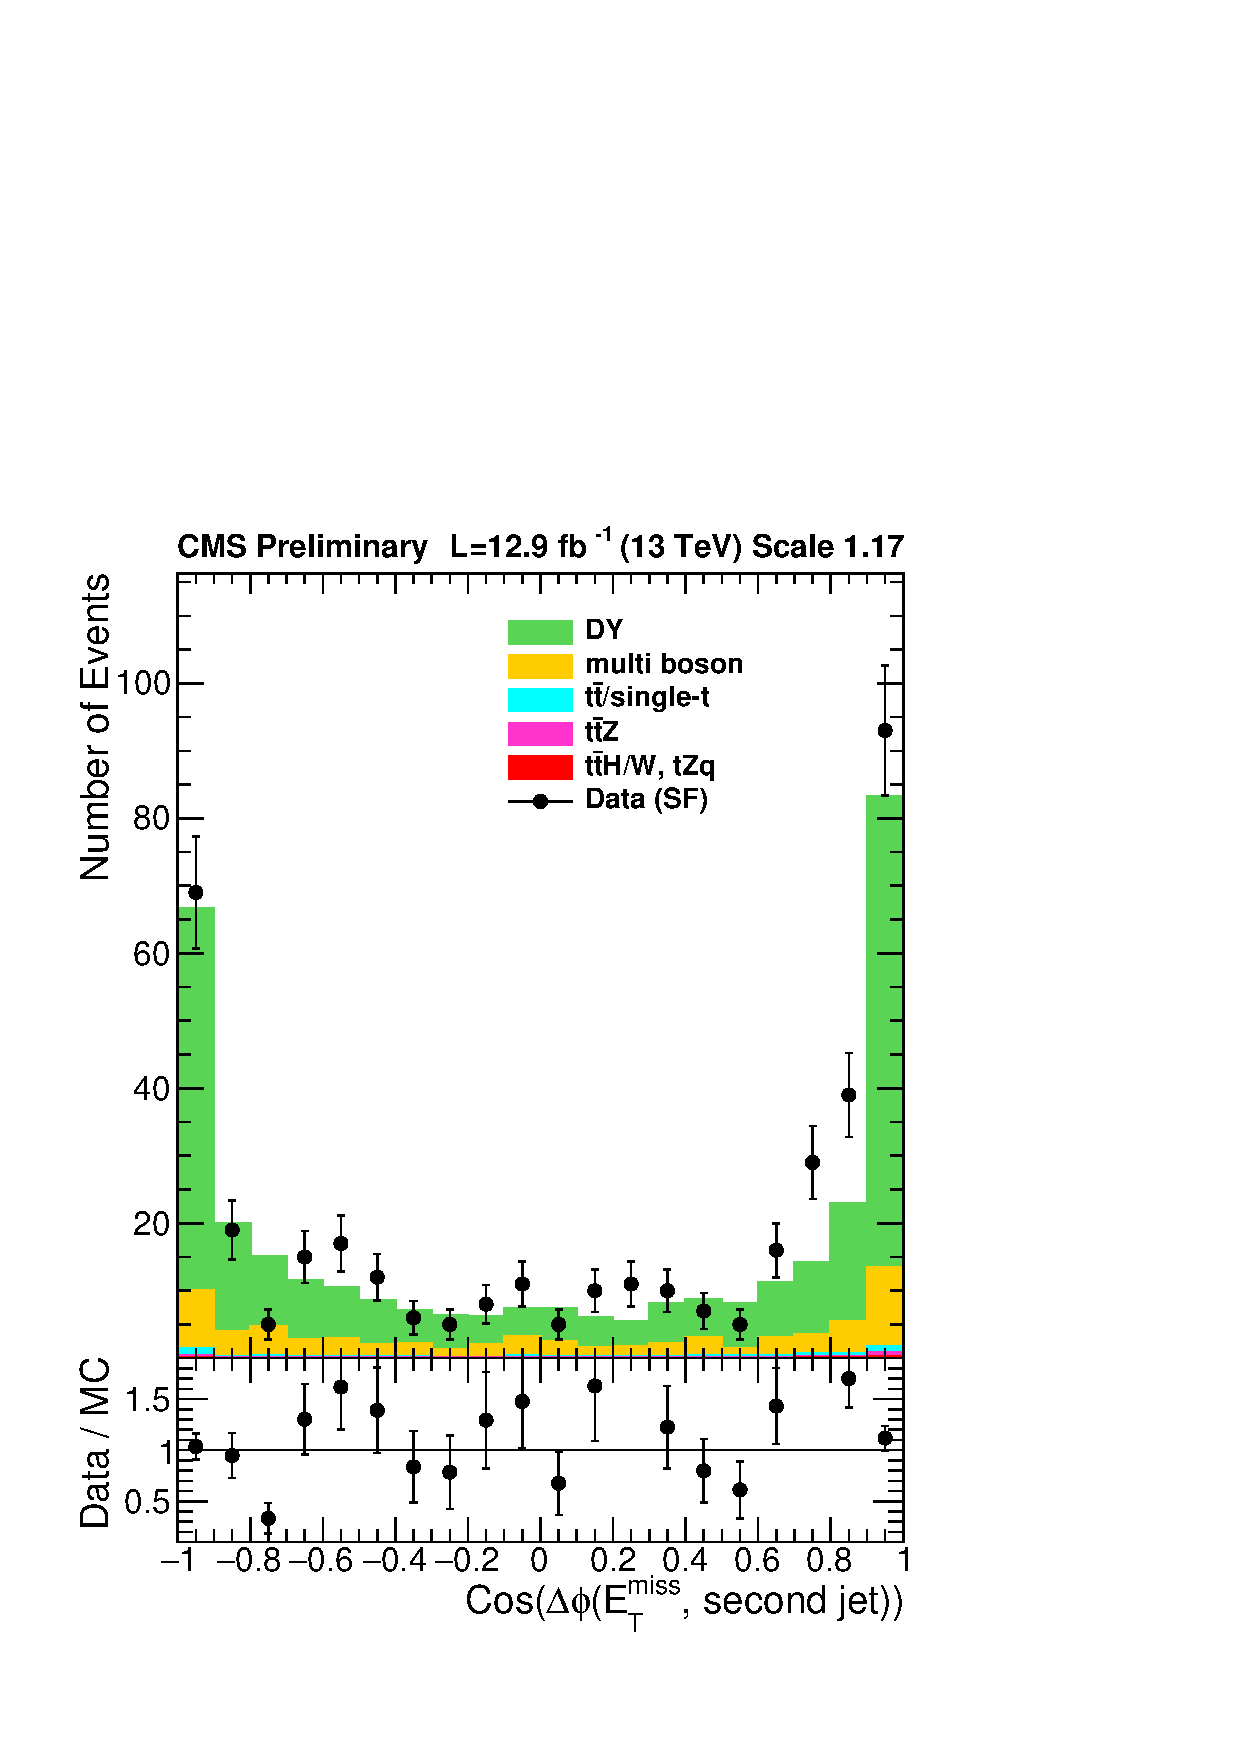
\includegraphics[width=0.45\textwidth]{figures/analysisPlots/SF/njet2-btag0-multiIsoWP-looseLeptonVeto-mll20-onZ-met80-mt2ll100/cosMetJet2phi_smallBinning.pdf}}
\caption{Distributions of \metSig, \mtll for same-flavour ($ee$/$\mu\mu$) events falling within the $Z$-mass window, with two jets and exactly 0 $b$-tags, $\met > 80$ GeV
     and $\mtll > 100$ GeV.}
\label{fig:DY}
\end{figure}

\begin{figure}[!hbtp]
\centering
\subfloat[$\cos{\Delta\phi(\met, \text{leading jet})}$]{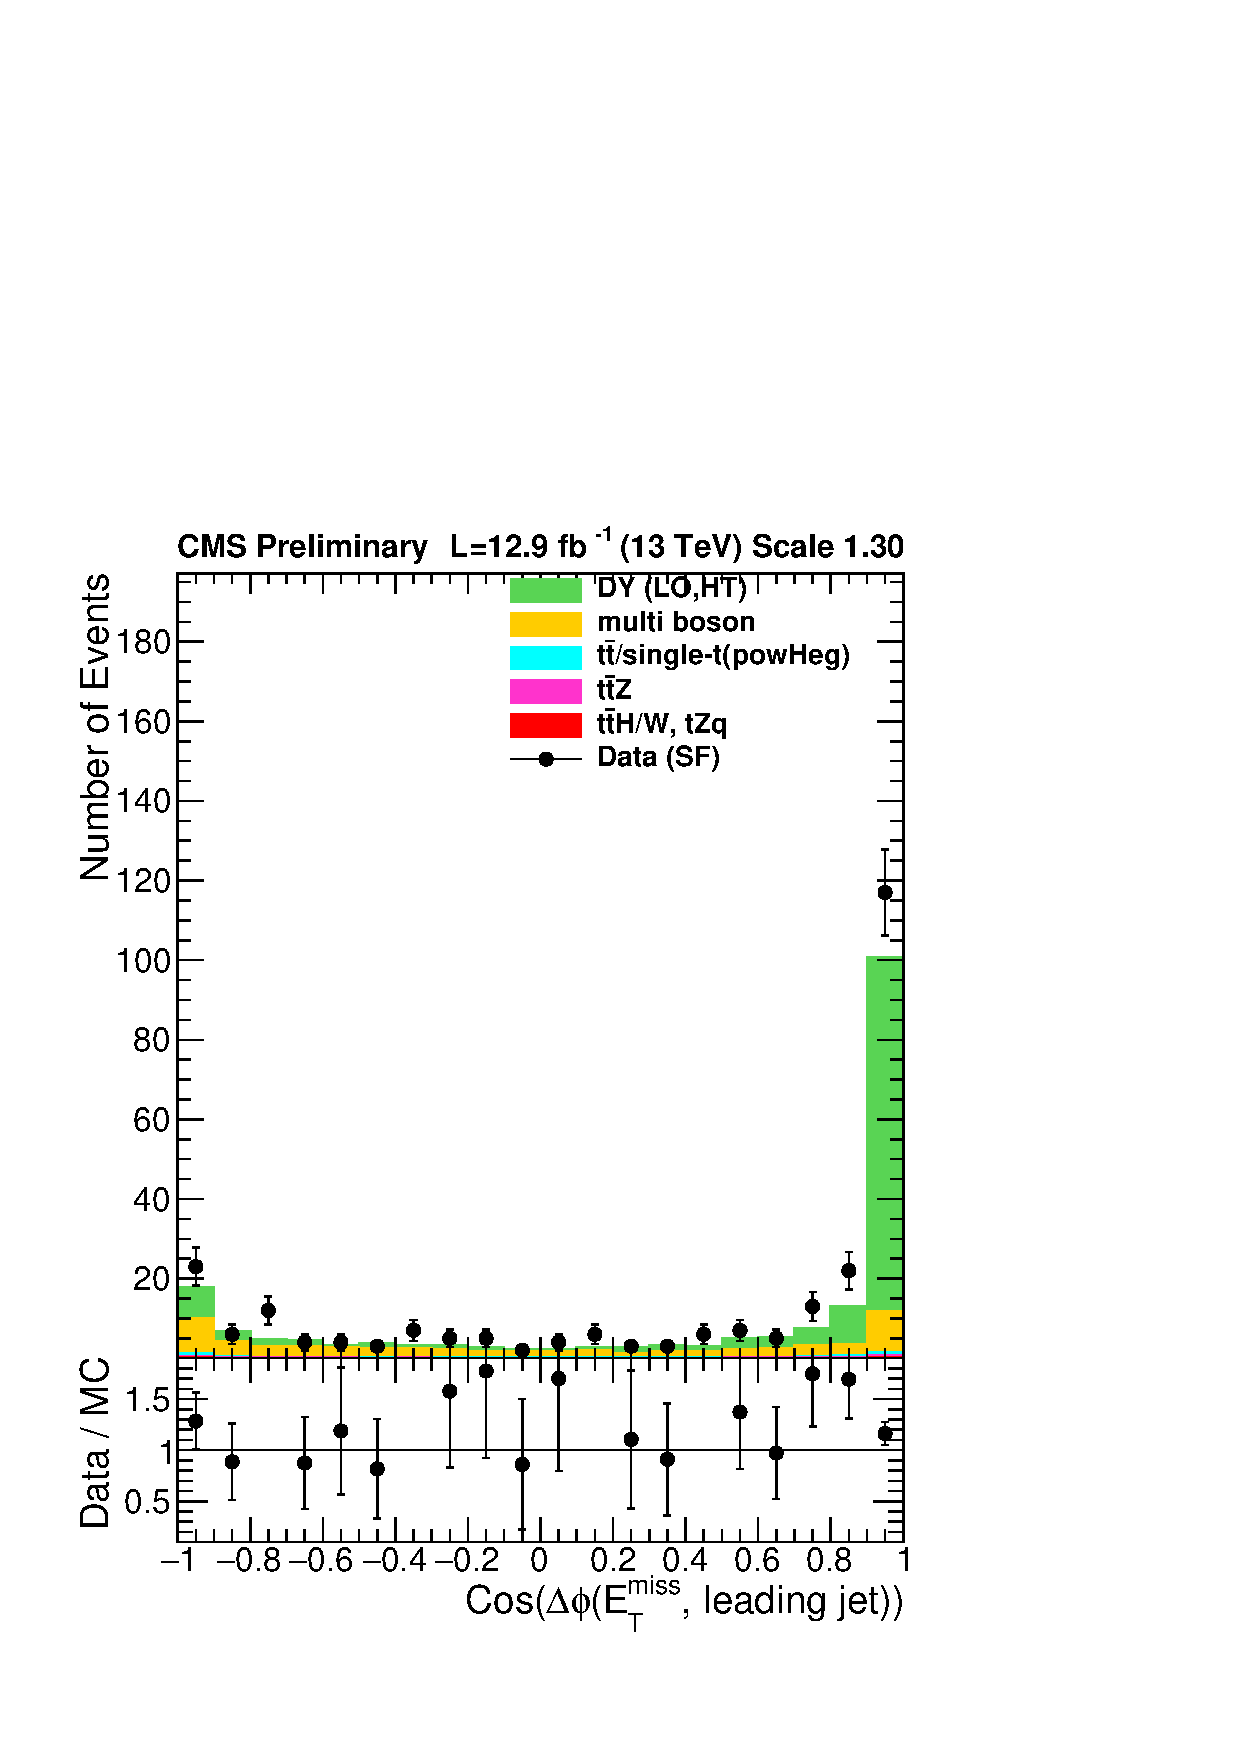
\includegraphics[width=0.4\textwidth]{figures/analysisPlots/SF/njet2-btag0-multiIsoWP-looseLeptonVeto-mll20-onZ-met80-metSig5-mt2ll100/cosMetJet1phi_smallBinning.pdf}}
\subfloat[$\cos{\Delta\phi(\met, \text{2nd leading jet})}$]{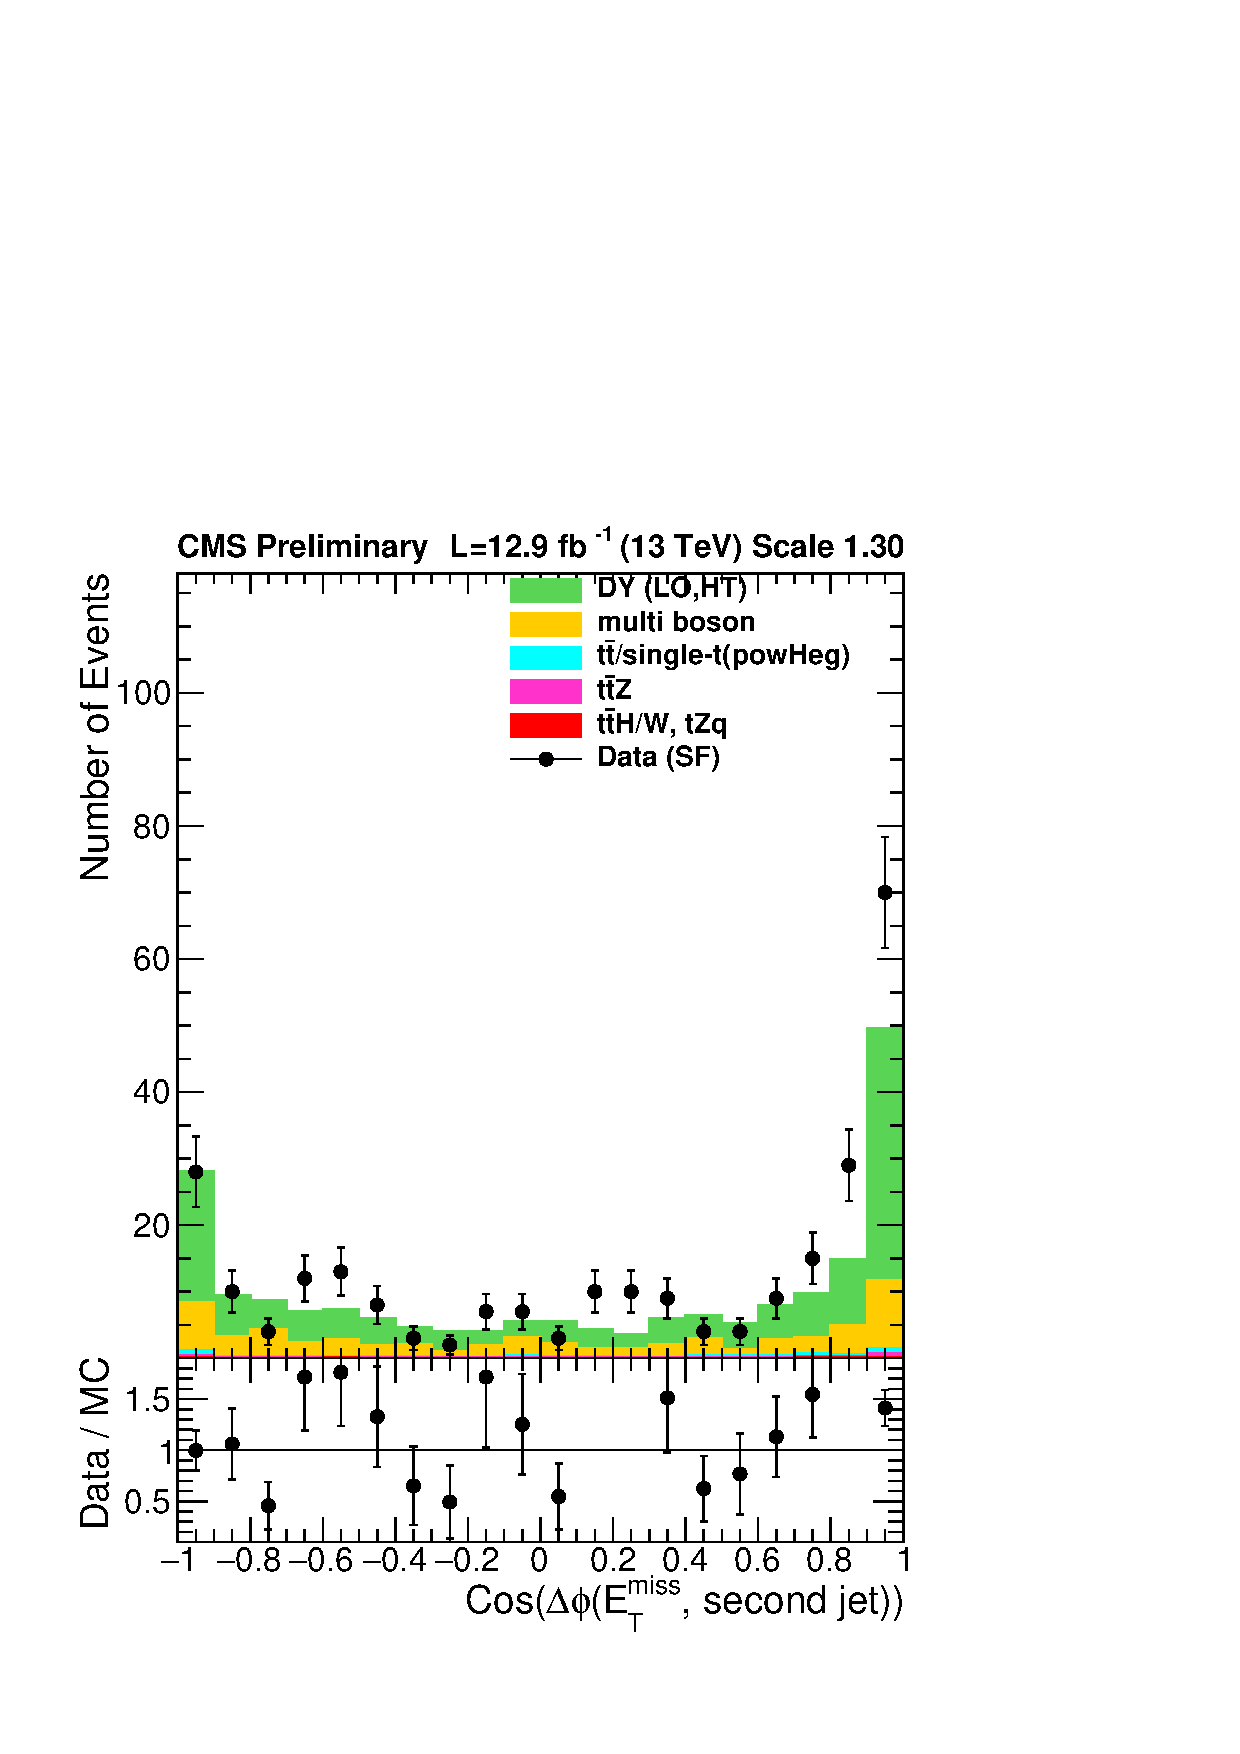
\includegraphics[width=0.4\textwidth]{figures/analysisPlots/SF/njet2-btag0-multiIsoWP-looseLeptonVeto-mll20-onZ-met80-metSig5-mt2ll100/cosMetJet2phi_smallBinning.pdf}}
\caption{Distributions of $\cos{\Delta\phi(\met, \text{jet})}$ for same-flavour ($ee$/$\mu\mu$) events falling within the $Z$-mass window, with two jets and exactly 0 $b$-tags, $\met > 80$ GeV, $S > 5$
     and $\mtll > 100$ GeV.}
\label{fig:DY_afterMetSig}
\end{figure}


\begin{figure}[!hbtp]
\centering
\subfloat[$\cos{\Delta\phi(\met, \text{leading jet})} > 0.8$ or $\cos{\Delta\phi(\met, \text{2nd leading jet})} > \cos{0.25}$][$\cos{\Delta\phi(\met, \text{leading jet})} > 0.8$ or \\ $\cos{\Delta\phi(\met, \text{2nd leading jet})} > \cos{0.25}$]{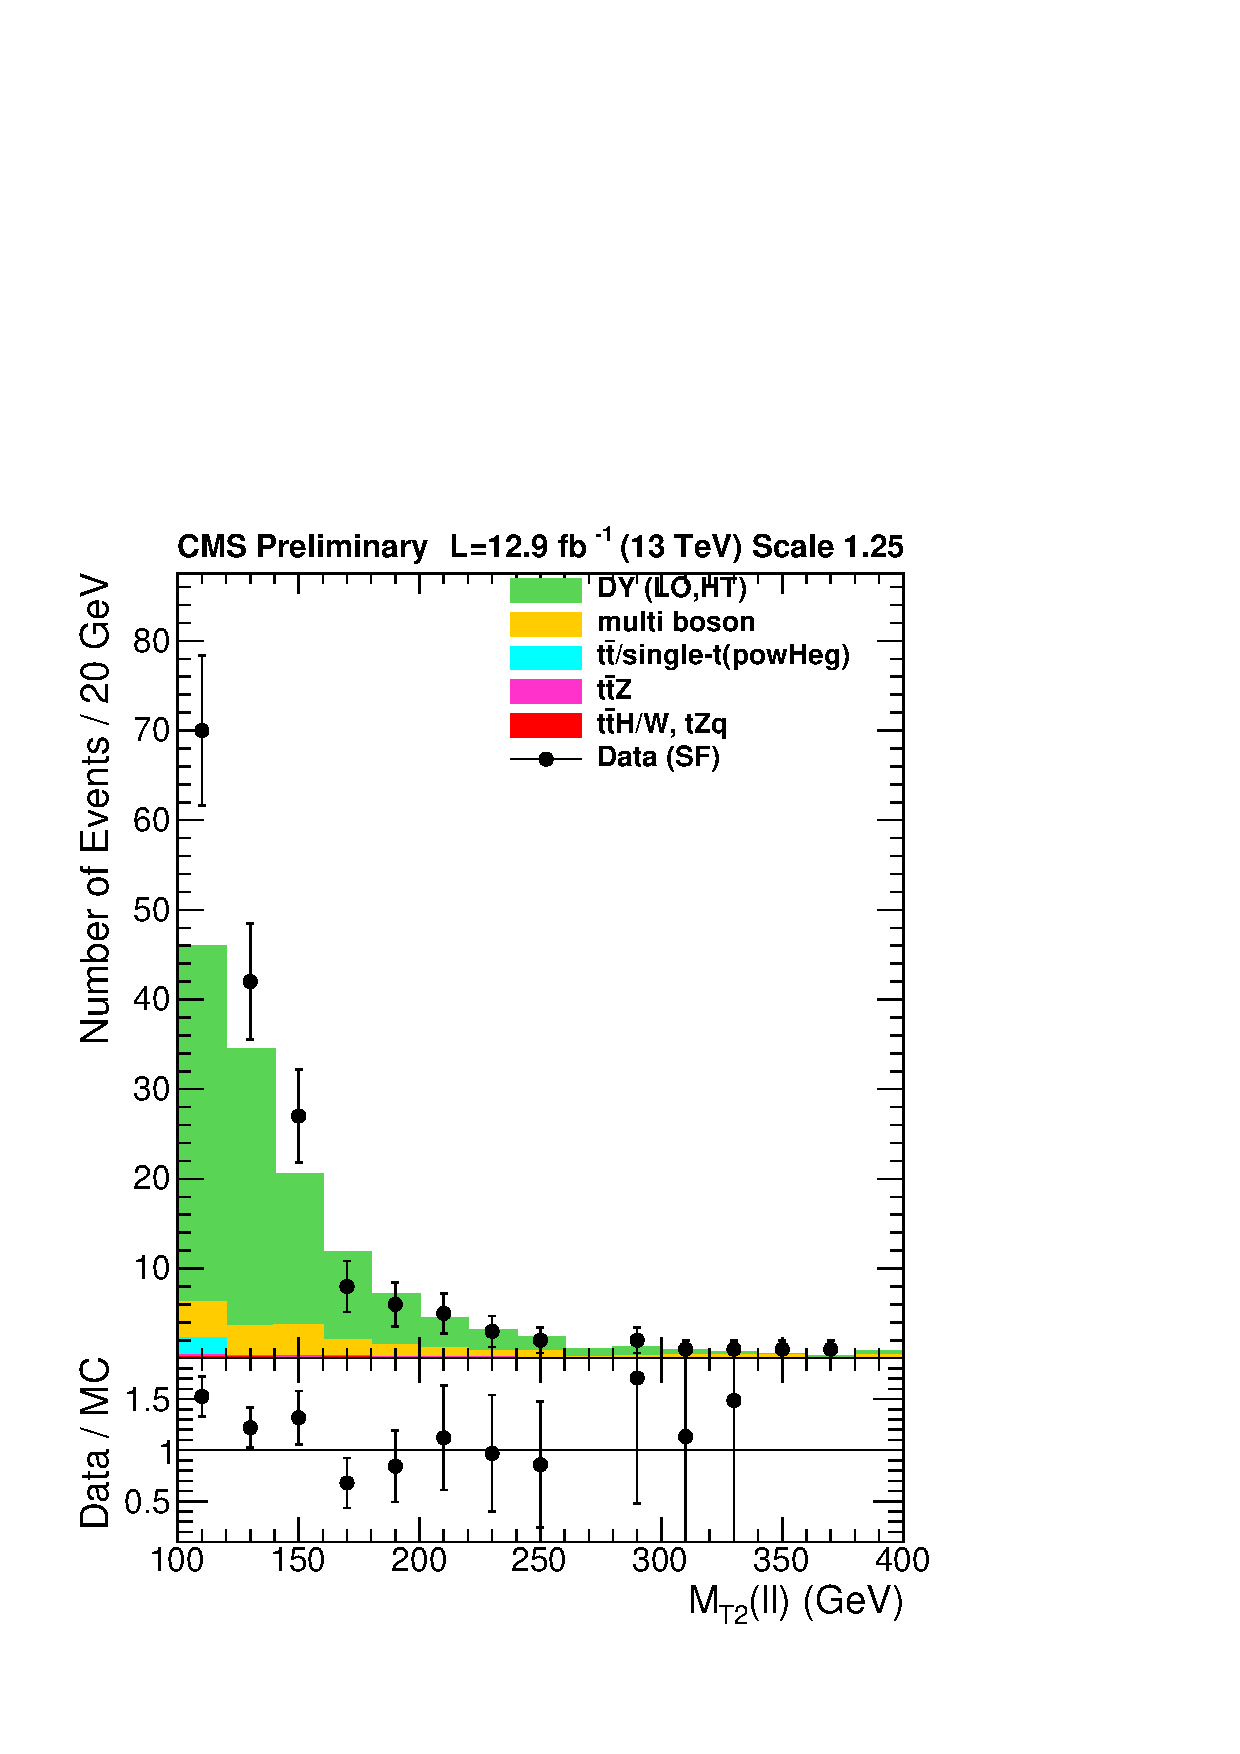
\includegraphics[width=0.4\textwidth]{figures/analysisPlots/SF/njet2-btag0-multiIsoWP-looseLeptonVeto-mll20-onZ-met80-metSig5-dPhiInv-mt2ll100/dl_mt2ll.pdf}}
\subfloat[$\cos{\Delta\phi(\met, \text{leading jet})} < 0.8$ and $\cos{\Delta\phi(\met, \text{2nd leading jet})} < \cos{0.25}$][$\cos{\Delta\phi(\met, \text{leading jet})} < 0.8$ and \\ $\cos{\Delta\phi(\met, \text{2nd leading jet})} < \cos{0.25}$]{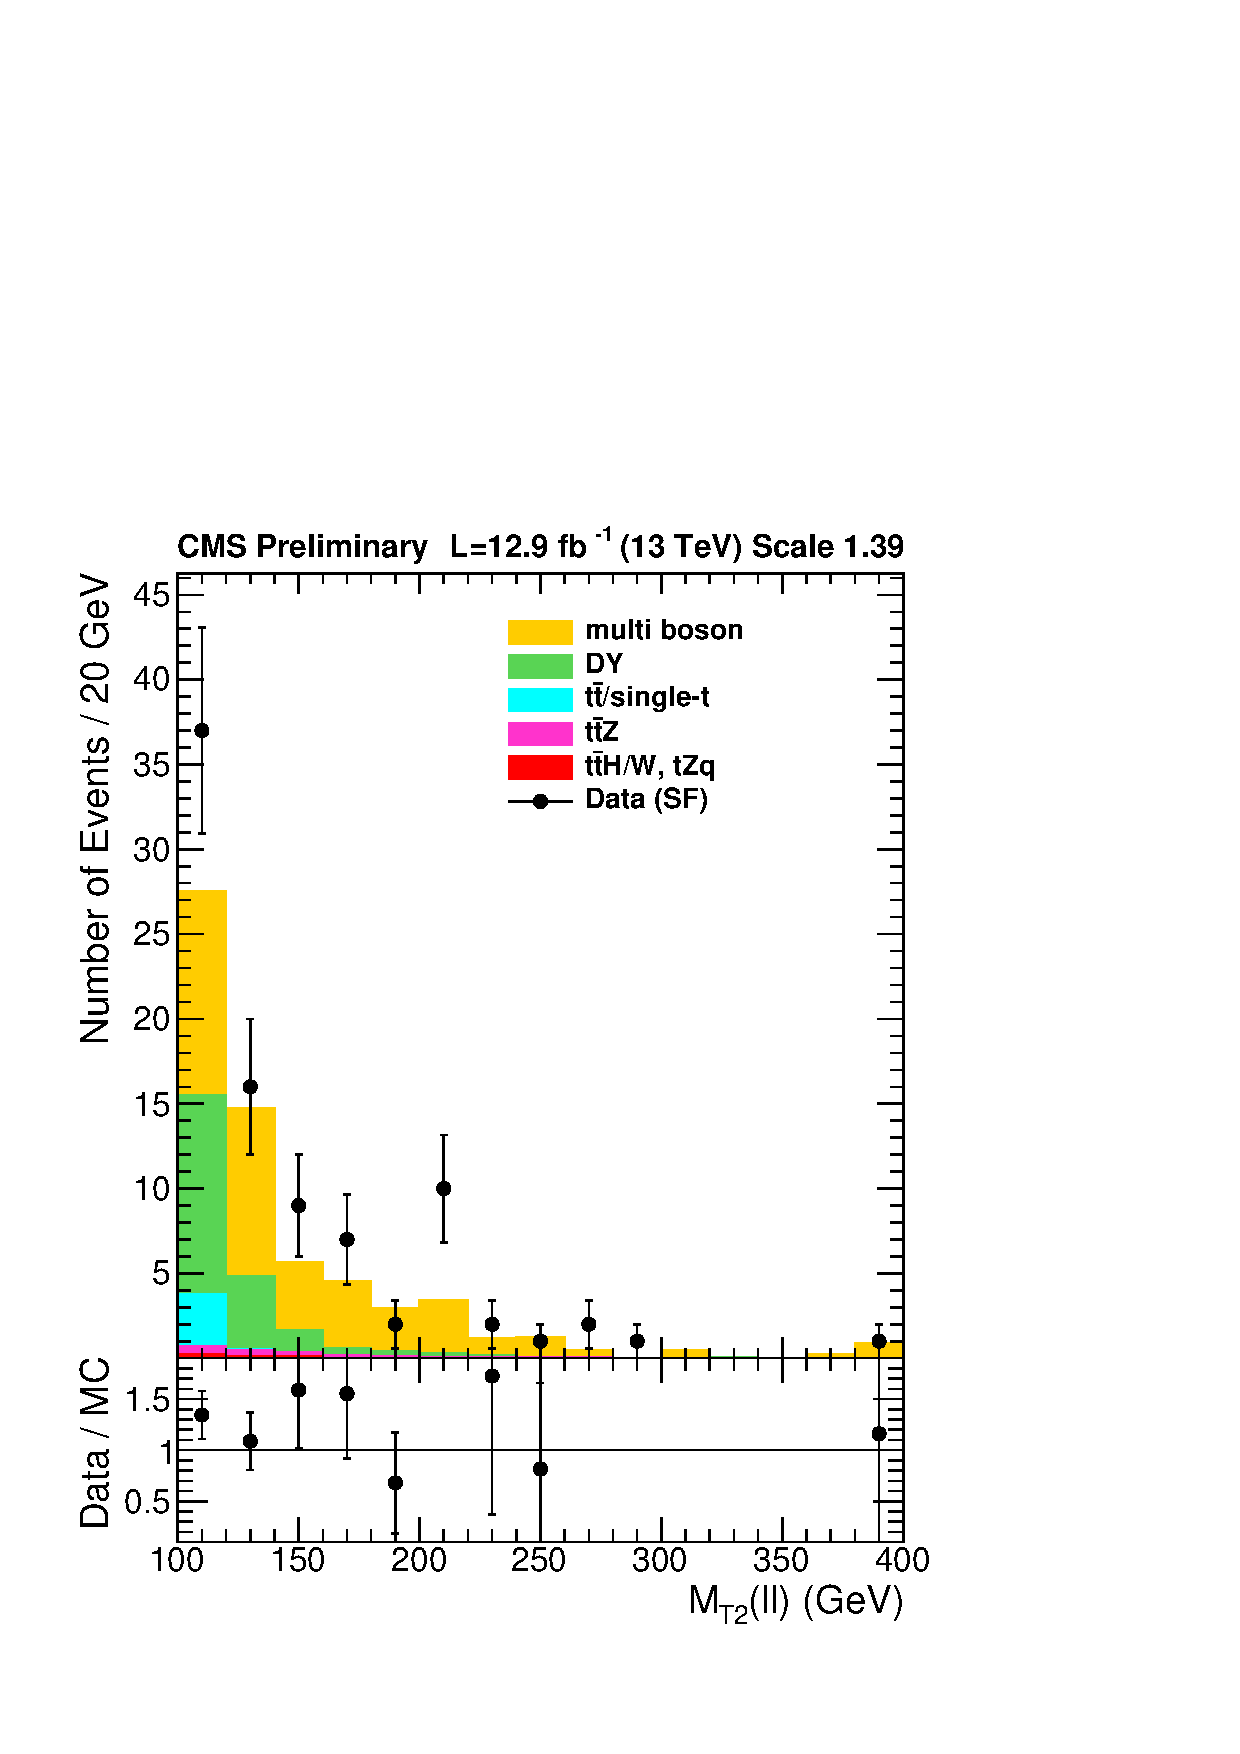
\includegraphics[width=0.4\textwidth]{figures/analysisPlots/SF/njet2-btag0-multiIsoWP-looseLeptonVeto-mll20-onZ-met80-metSig5-dPhiJet0-dPhiJet1-mt2ll100/dl_mt2ll.pdf}}
\caption{Distributions of \mtll in a DY and diboson dominated region for same-flavour ($ee$/$\mu\mu$) events falling within the $Z$-mass window, with two jets and exactly 0 $b$-tags, $\met > 80$ GeV, \metSig $> 5$
     and $\mtll > 100$ GeV.}
\label{fig:DY_dPhiInv}
\end{figure}

\begin{table}
\centering
%\scriptsize
\begin{tabular}{l|ccccccc} 
  selection & DY&TTJets&multiBoson&TTX&observed&DY purity \\ 
  \hline 
  $\met > 50$ GeV & 837.96 & 6.12 & 87.76 & 4.98 & 1052&                                         $89\%$\\ %$1.14\pm0.04$ &
  $\met > 80$ GeV & 261.25 & 5.65 & 64.57 & 3.89 & 392&                                          $77\%$\\ %$1.22\pm0.08$ &
  $\met > 50$ GeV, $\metSig > 5$ & 179.30 & 5.40 & 59.83 & 3.47 & 346&                           $72\%$\\ %$1.55\pm0.11$ &
  $\met > 80$ GeV, $\metSig > 5$ & 132.20 & 5.13 & 57.34 & 3.38 & 257&                           $66\%$\\ %$1.45\pm0.13$ &
  $\met > 50$ GeV, inv. $\Delta\phi$ & 656.29 & 2.38 & 39.14 & 2.26 & 776&                       $94\%$\\ %$1.12\pm0.04$ &
  $\met > 80$ GeV, inv. $\Delta\phi$ & 217.04 & 2.14 & 22.92 & 1.61 & 265&                       $89\%$\\ %$1.10\pm0.08$ &
  $\met > 50$ GeV, $\metSig > 5, \Delta\phi$ & 28.02 & 3.29 & 40.17 & 2.11 & 100&                $37\%$\\ %$1.94\pm0.38$ &
  $\met > 80$ GeV, $\metSig > 5, \Delta\phi$ & 18.45 & 3.14 & 39.49 & 2.07 & 88&                 $29\%$\\ %$2.35\pm0.54$ &
  $\met > 50$ GeV, $\metSig > 5$, inv. $\Delta\phi$ & 151.28 & 2.12 & 19.66 & 1.36 & 246&        $86\%$\\ %$1.47\pm0.11$ &
  $\met > 80$ GeV, $\metSig > 5$, inv. $\Delta\phi$ & 113.75 & 1.99 & 17.85 & 1.31 & 169&        $84\%$\\ %$1.30\pm0.12$ &
\end{tabular} 

\caption{Yields and DY purity in 0b with the listed cuts applied on top of events falling within the $Z$-mass window, having two jets and exactly 0 $b$-tags, and $\mtll > 100$ GeV}
\label{table:scalefactorsDY}
\end{table}

To quantify the robustness of the scale factor we first consider Fig.~\ref{fig:DY_nbtag} which shows a large fraction of DY events without generated (defined as \texttt{hadronFlavour} of $\pm 5$ \cite{twiki:hadronFlavour}) b-quarks entering the $\Nbtags\geq 1$ region. 
The uncertainties on events with only fake b tags are covered by the experimental uncertainties provided by the BTV POG. 
\begin{figure}[!hbtp]
\centering
\subfloat[\Nbtags]{\includegraphics[width=0.45\textwidth]{figures/DY/dy_nbtag.png}}
\caption{Distributions of \Nbtags in simulated DY events in events with and without generated b-quarks.}
\label{fig:DY_nbtag}
\end{figure}
In order to assess the uncertainties on the generated b-quark multiplicity we calculate  the variation of ratios as a function of the {\texttt NNPDF} weights and find a 2\% variation. 
Furthermore, we scale the events with generated b-quarks up and down by 50\% to cover the uncertainty on the modeling of gluon splitting. This translates into an uncertainty~of~25\%~on~$R$. 

In a second step, we invert the requirements on the angular separation of \ETmiss and jets and consequently obtain a region that is dominated by diboson backgrounds as seen in Fig.~\ref{fig:DY_dPhiInv}b.
The purity of diboson backgrounds is approximately 70\%. 
Applying the scale factor $R$ on DY and subtracting again simulated yields from data, we calculate a scale factor of $1.45\pm0.26$ for the diboson background and we add a 25\% uncertainty on the DY component. 
As the DY and diboson scale factors are used to correct the simulation based prediction, their uncertainty is propagated to every signal region in a correlated way.
For completeness, we list the composition of several selections in the on-Z selection with 0 b-tags in Table~\ref{table:scalefactorsDY}. 

%lists the measured scalefactors for different configurations of \met, \metSig and $\Delta\phi(\met, \text{jet})$ cuts. It is not possible to take exactly the same \met cuts
%as in the main analysis, given that very few DY events pass these cuts in combination with the $\mtll > 100 GeV$ requirement. 
%In order to achieve a $\mtll > 100 GeV$ region where DY dominates with sufficient statistics, we need to relax the \met and \metSig cuts and/or invert the $\Delta\phi(\met, \text{jet})$ cuts.
%Given that the region with $\met > 80$ GeV, $\metSig > 5$ and inverted $\Delta\phi$ cuts has a high purity, we choose this as our DY control region.
%Similarly, we derive a scalefactor of $1.45\pm0.26$ for dibosons using the $\met > 80$ GeV, $\metSig > 5$ and $\Delta\phi$ region where dibosons have a purity of 56 \%. While deriving the diboson scalfactors,the DY scalefactor was applied in the subtraction of the residual MC.

\begin{figure}[!hbtp]
\centering
\subfloat[inverted $\Delta\phi$ cuts and $\mtll>100$]{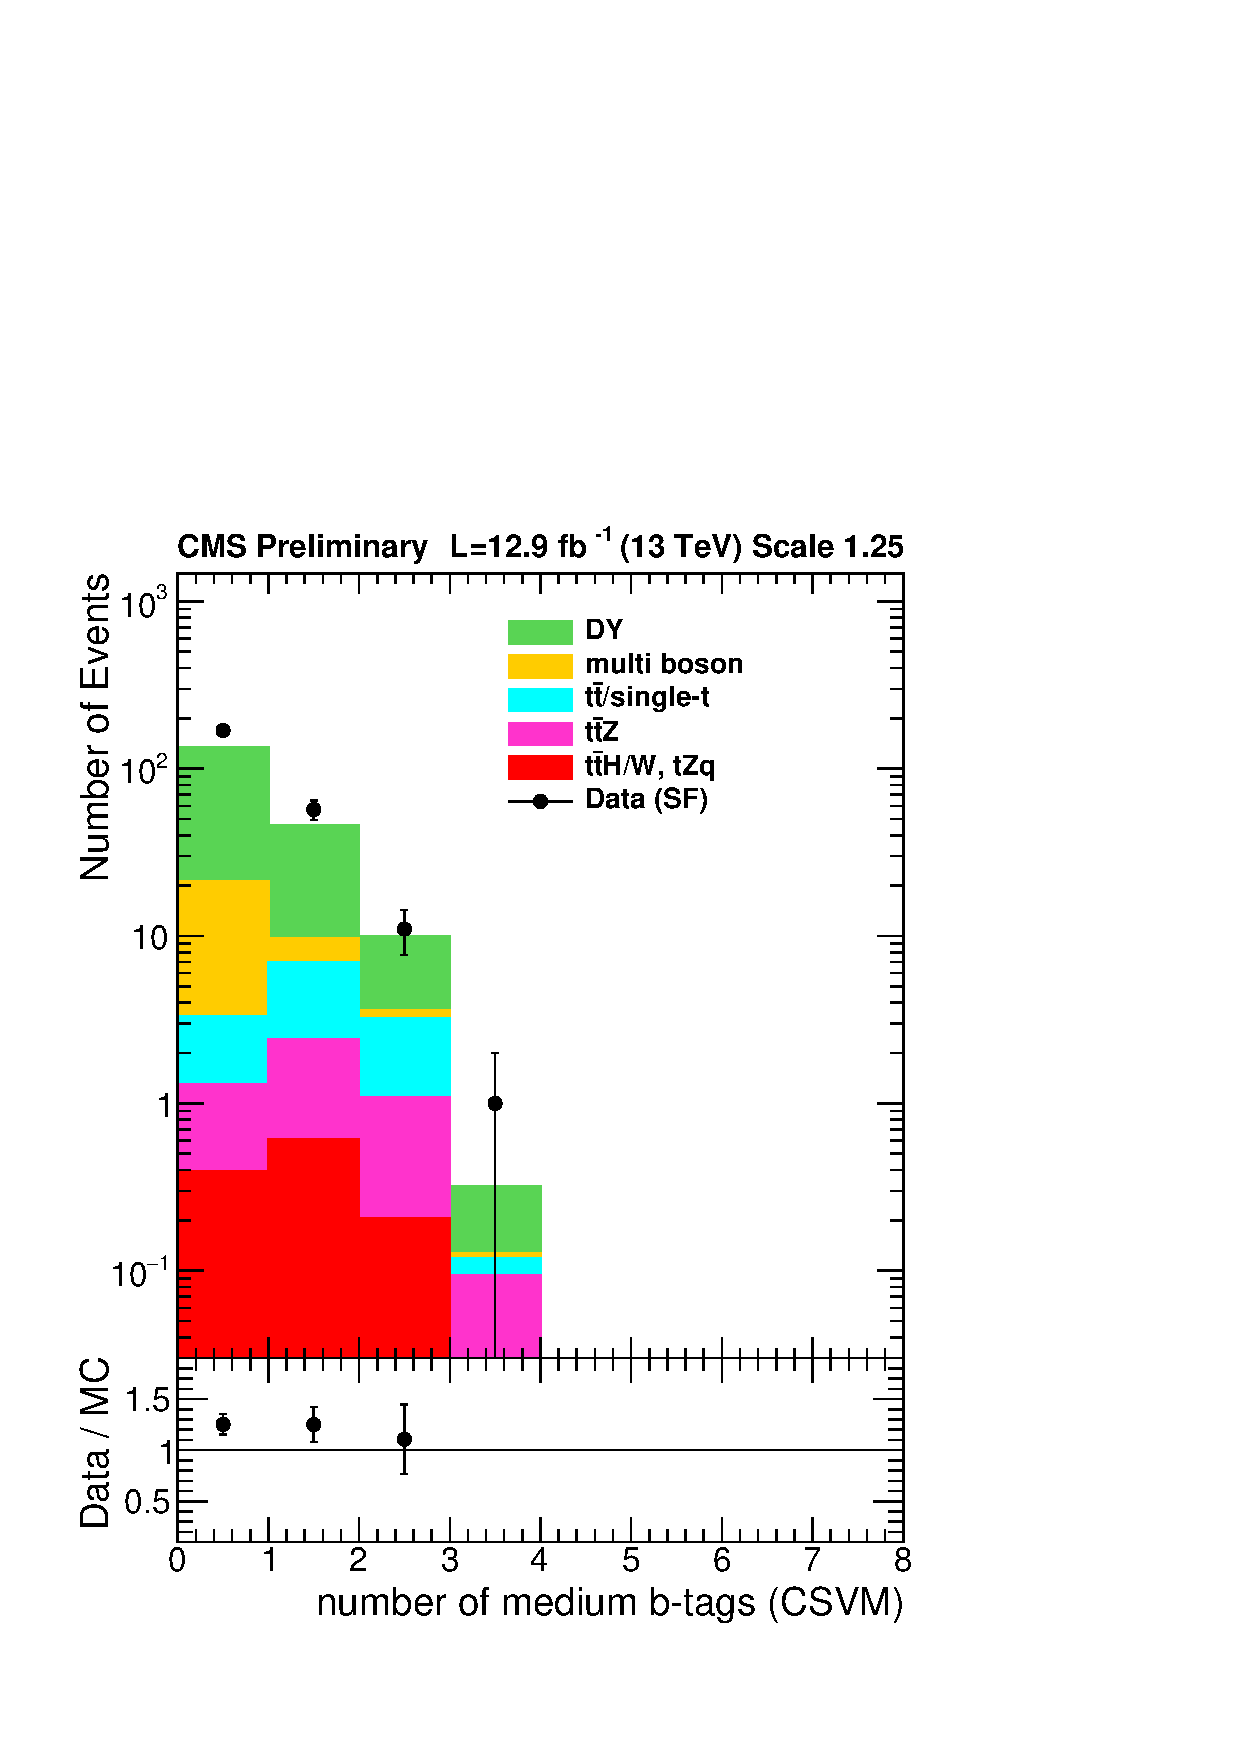
\includegraphics[width=0.45\textwidth]{figures/analysisPlots/SF_log/njet2-multiIsoWP-looseLeptonVeto-mll20-onZ-met80-metSig5-dPhiInv-mt2ll100/nBTag.pdf}}
\subfloat[inclusive]{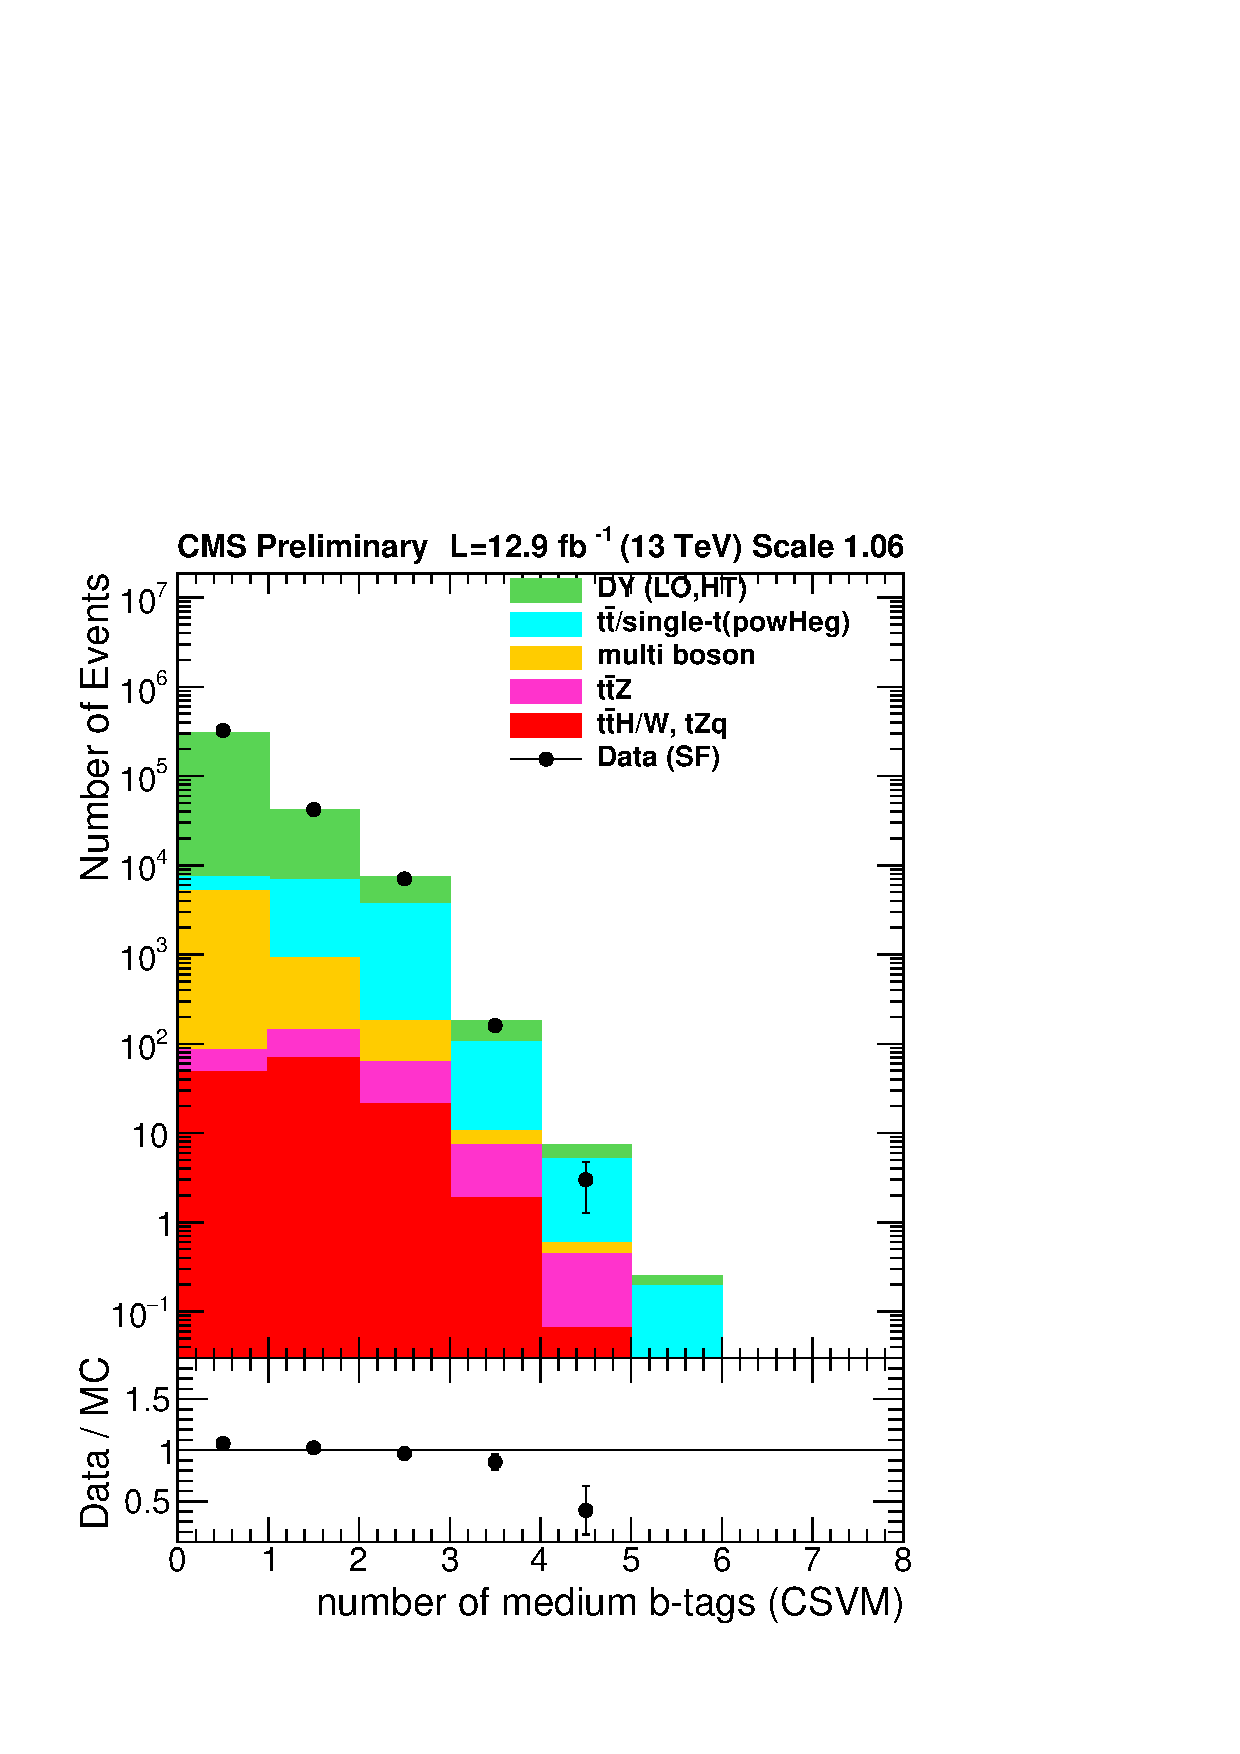
\includegraphics[width=0.45\textwidth]{figures/analysisPlots/SF_log/njet2-multiIsoWP-looseLeptonVeto-mll20-onZ/nBTag.pdf}}
\caption{Data/MC comparison of \Nbtags in the on-Z DY selection with $\mtll>100$~\GeV (left) and, inclusively, when removing the \mtll, \ETmiss, \metSig and $\Delta\phi$ requirements (right).}
\label{fig:DY_nbtag_validation}
\end{figure}


  \subsection{\texorpdfstring{$ttZ$}{TTZ} background estimation}

  One of our main backgrounds in the \mtll tail is $t\bar{t}Z$, in which the $Z$-boson decays into neutrinos. These neutrinos add additional missing energy to the event which promotes $t\bar{t}Z$ events
  from to bulk into the tail of the \mtll distribution. We use two complementary methods to verify the cross section normalization and \mtll shape description respectively.

  \subsubsection{Normalization in the \texorpdfstring{$t\bar{t}Z \to 3l$}{ttZ->3l} region}

    The normalization of the $t\bar{t}Z$ background could be estimated in a data-driven way using the $3l$ sideband, in which the \Z decays into two leptons, one top decays leptonically and the other hadronically:
    \begin{equation}
      t\bar{t}Z \to (bl\nu) (bjj) (ll) \nonumber 
    \end{equation}

    This measurement has recently performed~\citep{CMS-PAS-TOP-16-017}, measuring a signal strength parameter of 
    \begin{equation}
     0.89^{+0.18}_{-0.16} \text{(stat) }^{+0.14}_{-0.12}\text{(sys)}
    \end{equation}
    We use the measured
    signal strength as a scale factor for the $t\bar{t}Z$ MC and propagate its statistical and systematic errors into our analysis.
    The measurement requires the presence of three leptons exceeding respectively \pt thresholds of 30, 20 and 10 GeV.
    Two of these leptons are required to have the same flavour and opposite charge and should fall within a $Z$-mass window of 10 GeV in order to construct the $Z$-boson candidate.
    Additionally, we require at least three jets of which at least one has been identified as a $b$-jet.
    Figure~\ref{fig:ttz3l} shows the dilepton mass and b-jet distribution.

%    \begin{figure}
%      \centering
%      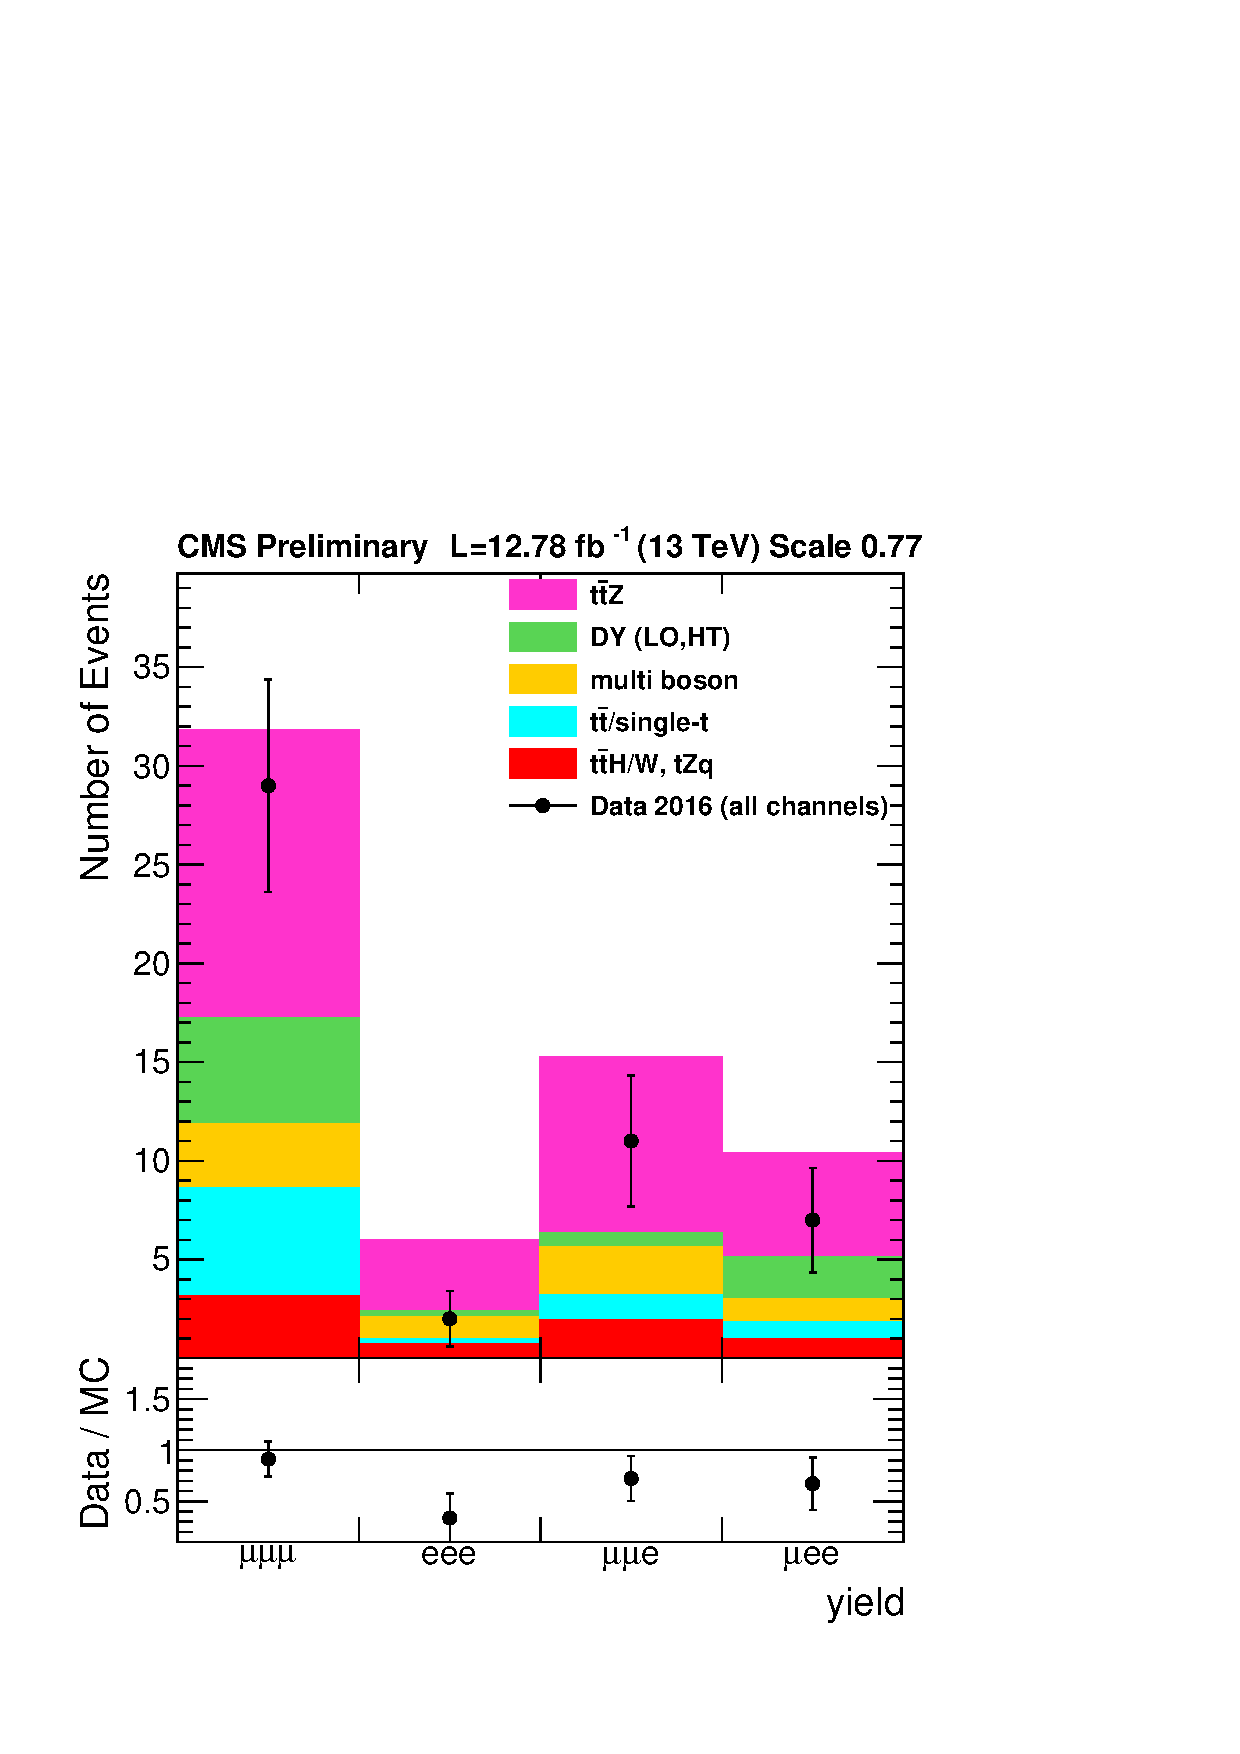
\includegraphics[width=0.7\textwidth]{figures/TTZ/all/njet3-nbtagLL-onZ-dR/yield.pdf}
%      \caption{Yields of the $t\bar{t}Z$ selection for the different 3-lepton channels}
%      \label{fig:ttz3l}
%    \end{figure}

    \begin{figure}
      \centering
      \includegraphics[width=0.45\textwidth]{figures/TOP-16-017/mll.png}
      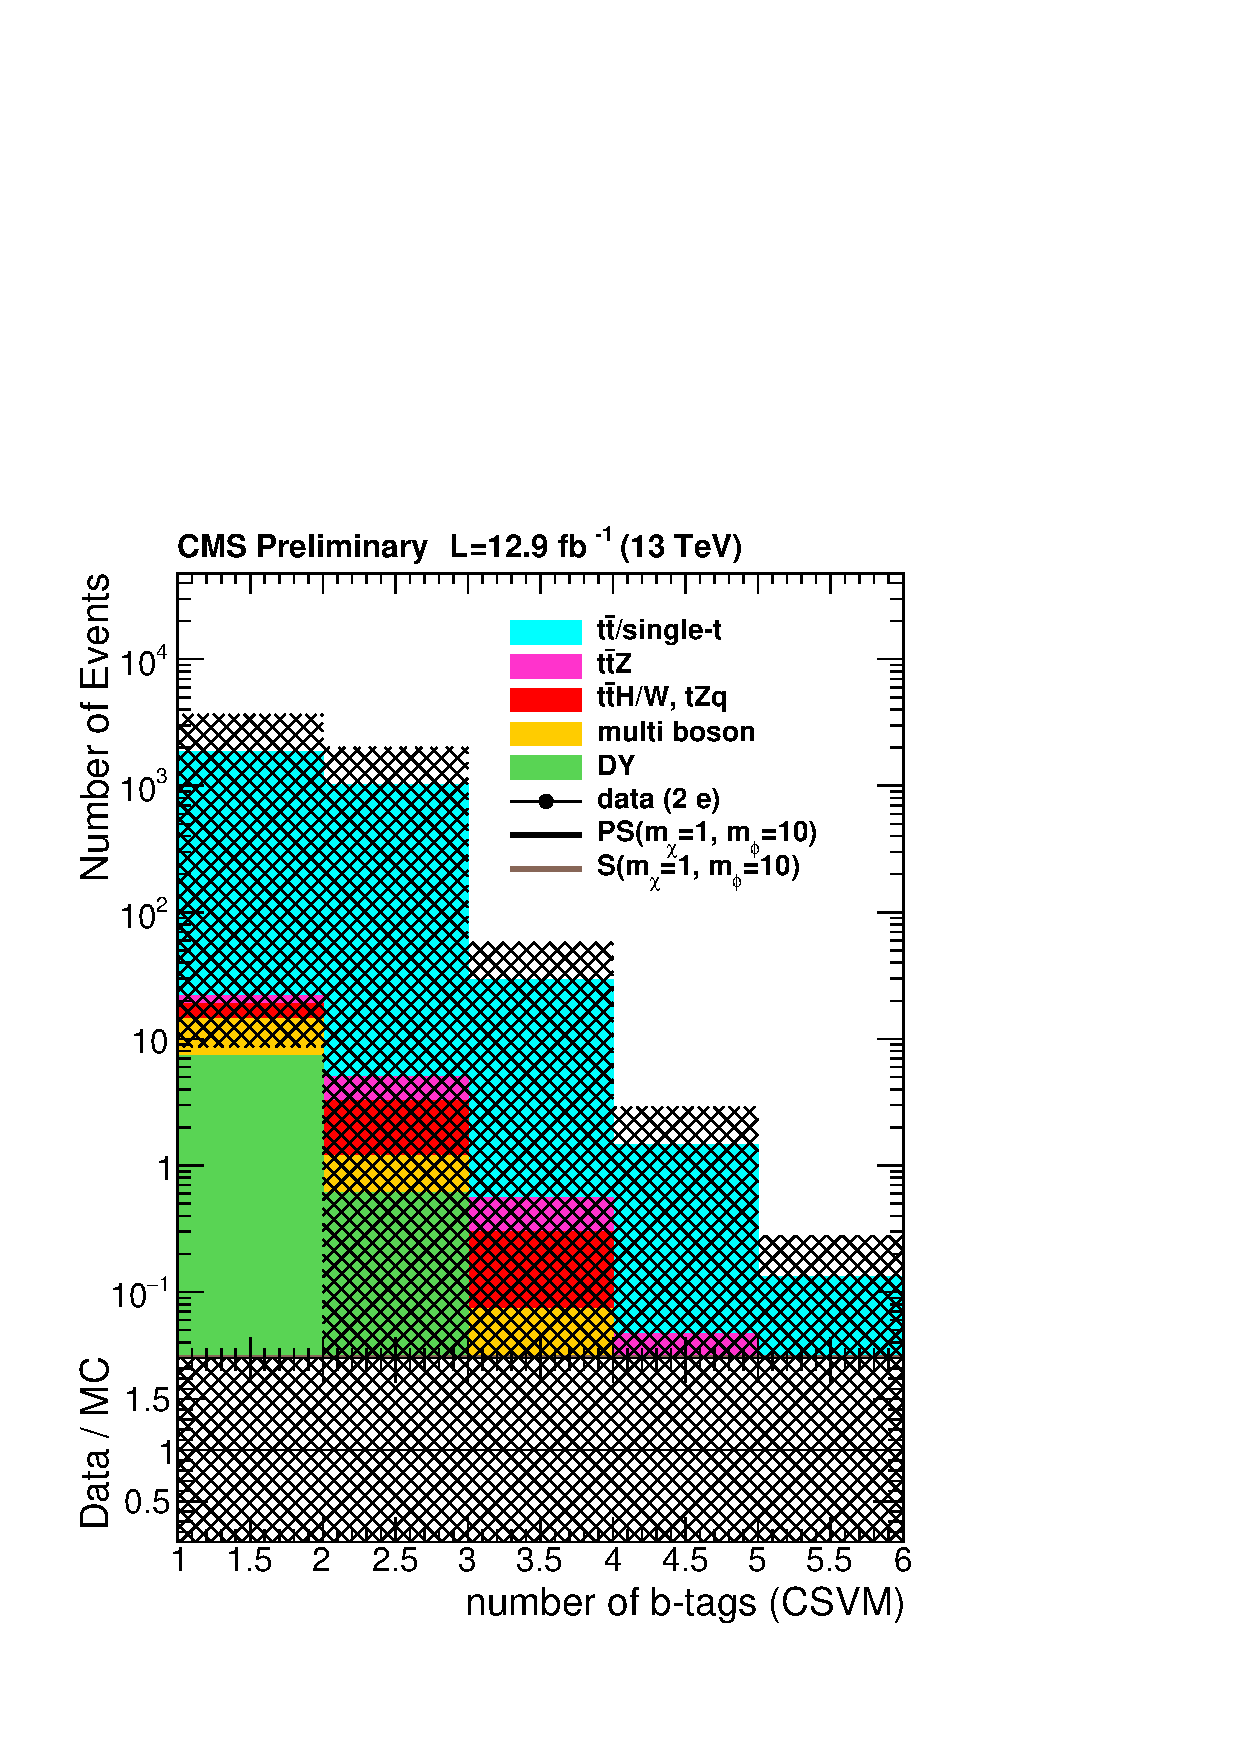
\includegraphics[width=0.45\textwidth]{figures/TOP-16-017/nbtags.png}
      \caption{Dilepton mass and b-jet distribution in the $t\bar{t}Z$ control region~\citep{CMS-PAS-TOP-16-017}}
      \label{fig:ttz3l}
    \end{figure}


  \subsubsection{Shape control region using \texorpdfstring{$tt\gamma$}{ttg} events}
    In order to verify the MC description of the \met and \mtll tails for the $t\bar{t}Z$ background, we select $t\bar{t}\gamma$ events in data and treat the photon \pt as additional missing energy
    such that it acts as a proxy for $t\bar{t}Z$ (\ie the photon \pt is vectorially added to the \met). Photons are selected according to Tab.~\ref{photonSelection}. Even though the kinematics of $t\bar{t}\gamma$ events differ from $t\bar{t}Z$ events due to the fact that the photon is massless, these kinematic
    differences could be mitigated by a reweighting of the boson \pt. Figure~\ref{fig:ttgGen} shows that the \met, \mtll, \mtlblb and \mtbb variables at generator-level between $t\bar{t}\gamma$ and $t\bar{t}Z$ are very similar
    after a bin-by-bin reweighting of the photon \pt to the $Z$ boson \pt,

    % GEN plots
    \begin{figure}
      \centering
      \subfloat[]{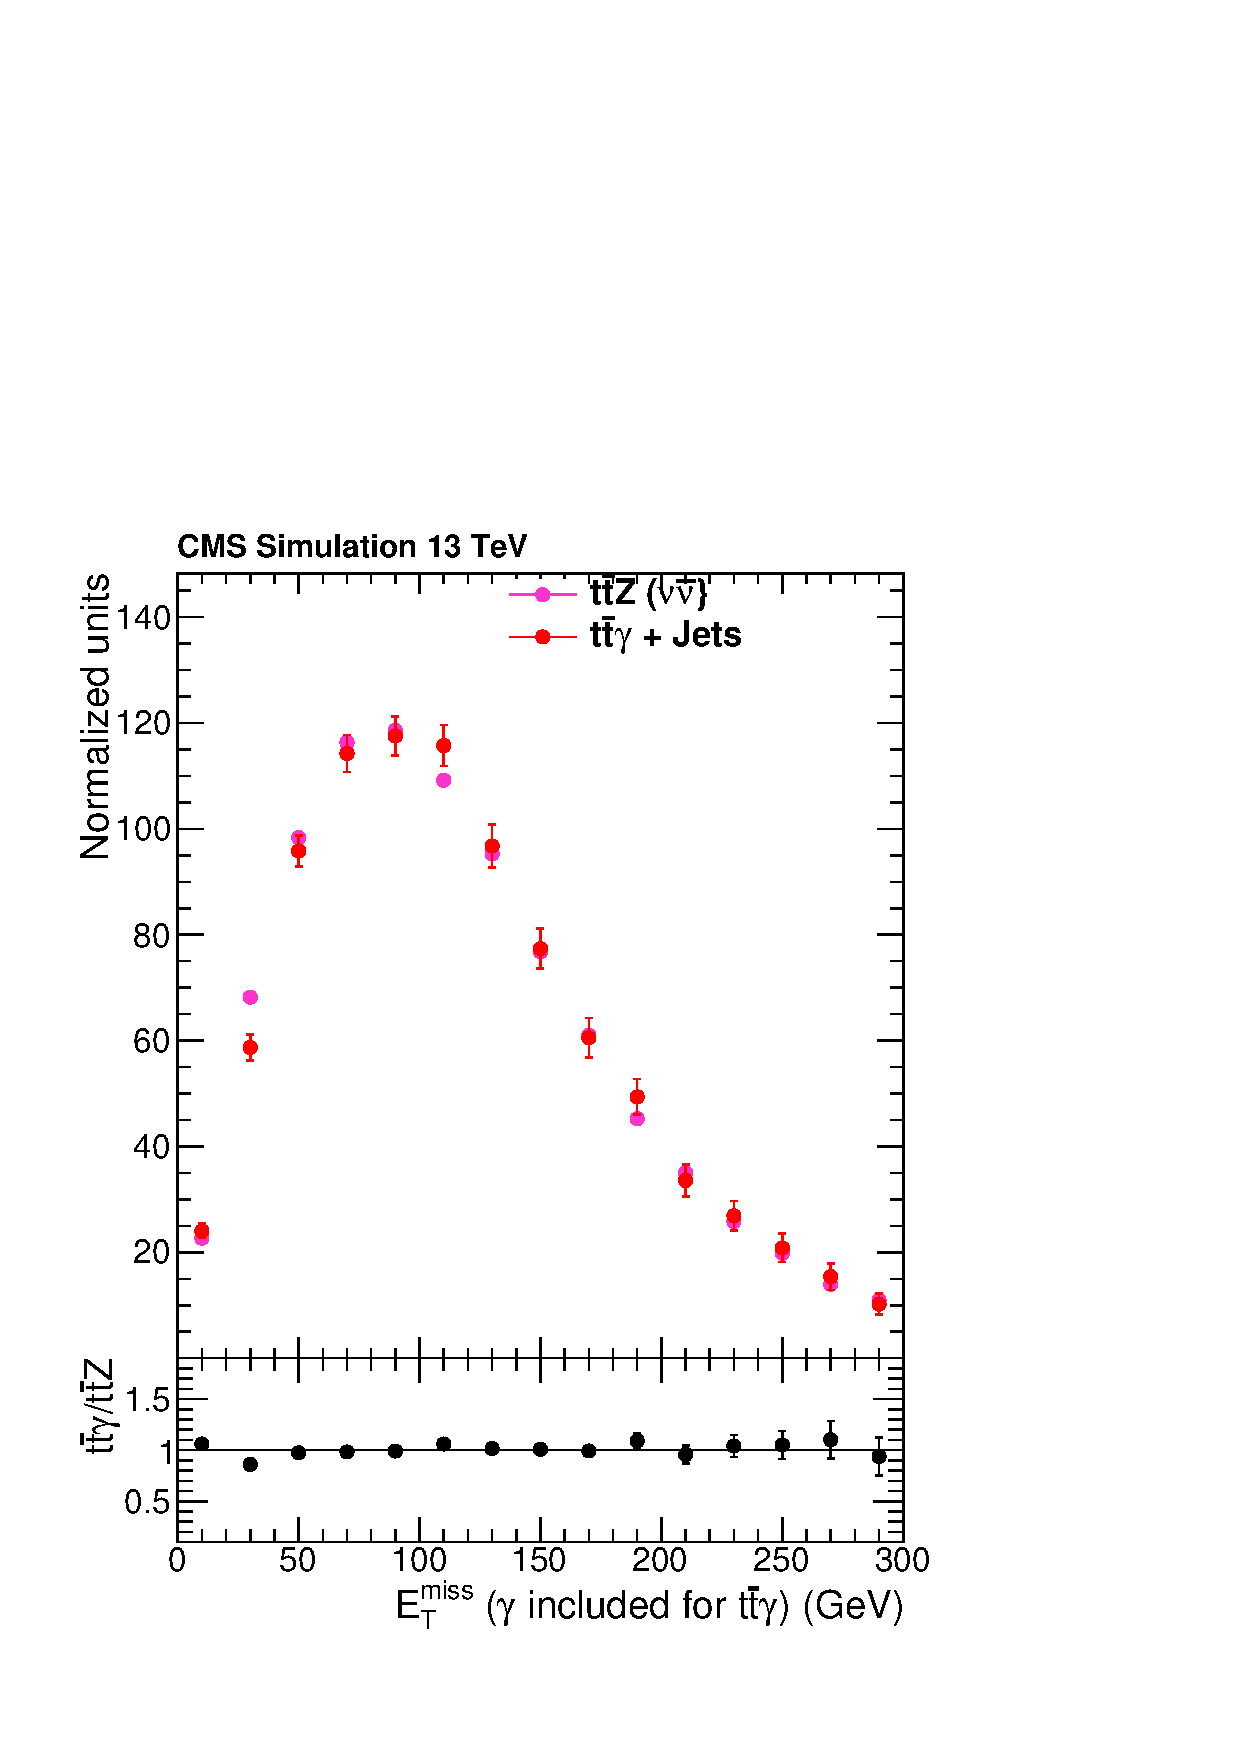
\includegraphics[width=0.45\textwidth]{figures/TTG_gen/reweighted/all_normalized/etaGamma25-ptGamma30/met_photonIncluded.pdf}}
      \subfloat[]{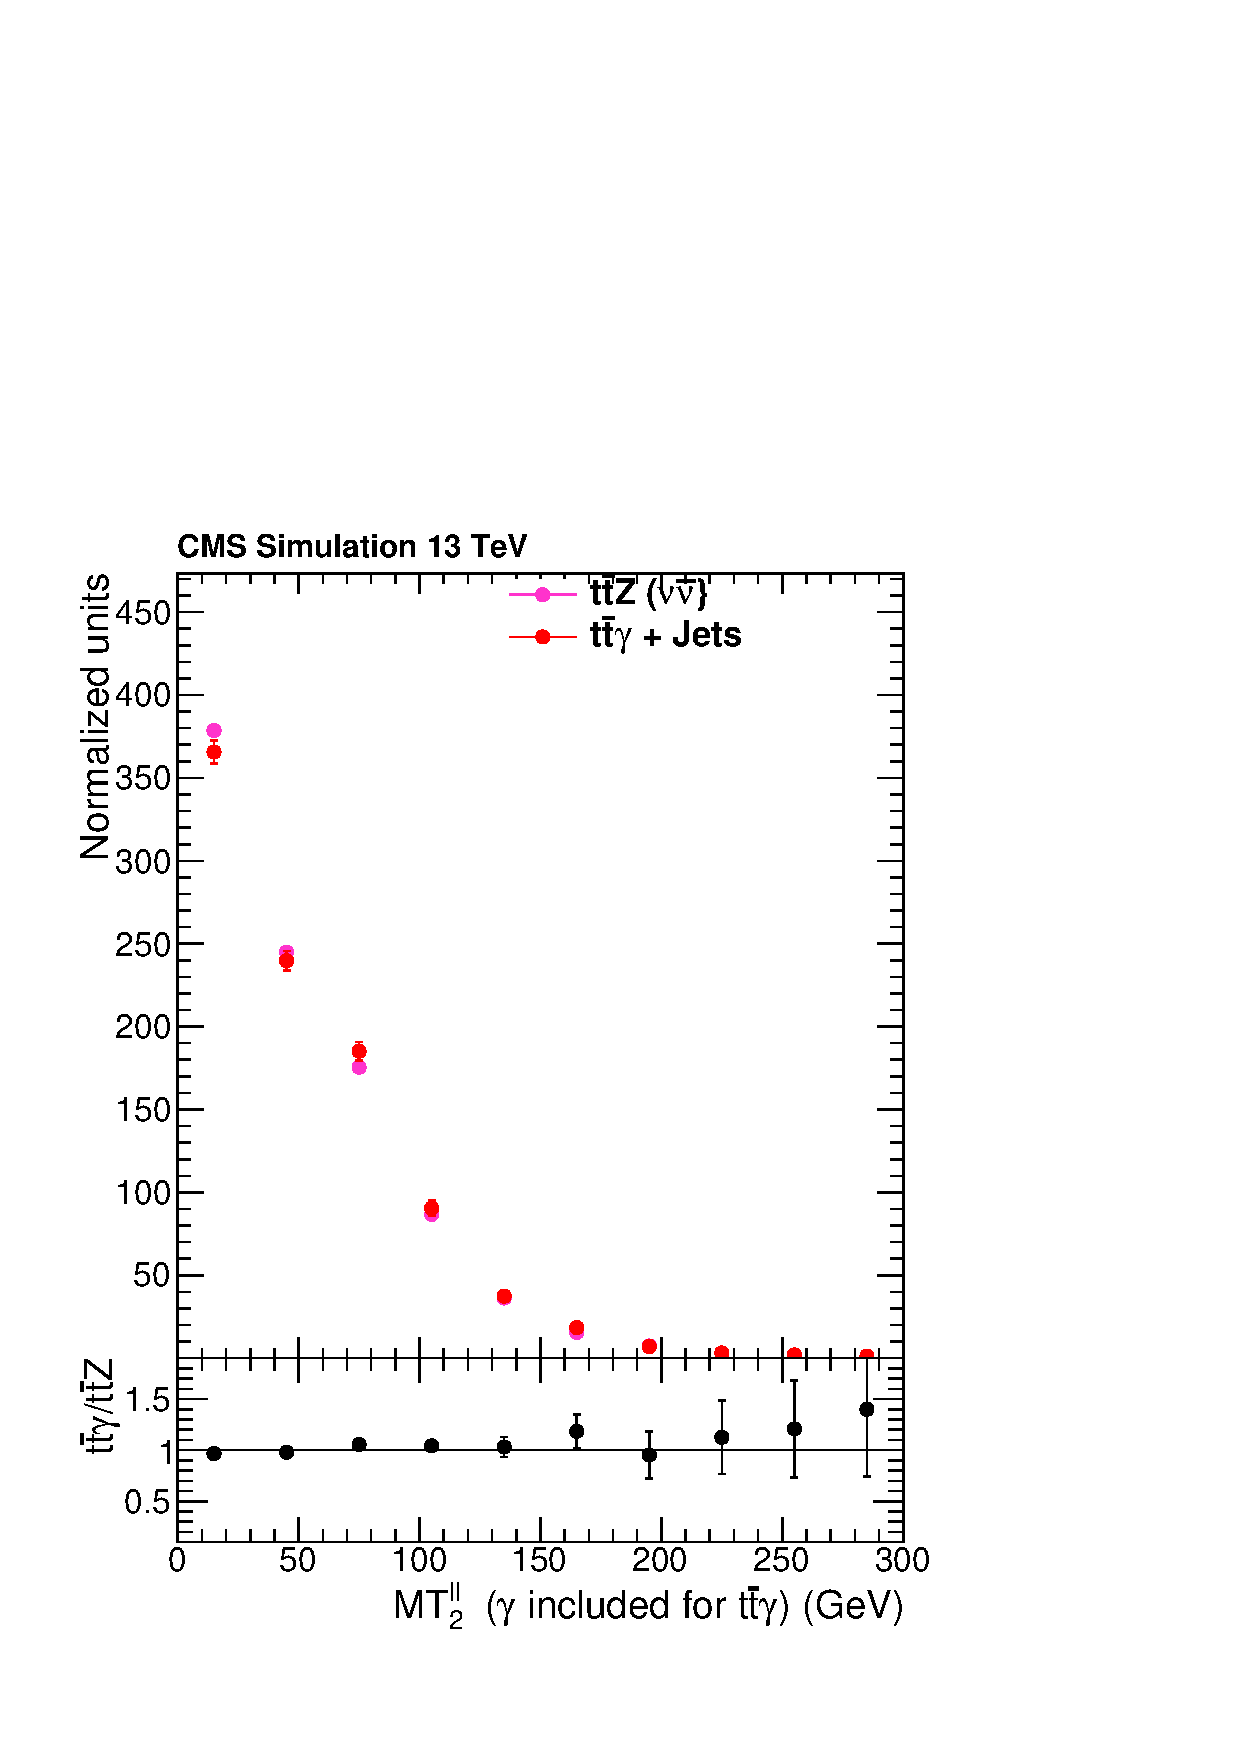
\includegraphics[width=0.45\textwidth]{figures/TTG_gen/reweighted/all_normalized/etaGamma25-ptGamma30/mt2ll_photonIncluded.pdf}}\\
      \subfloat[]{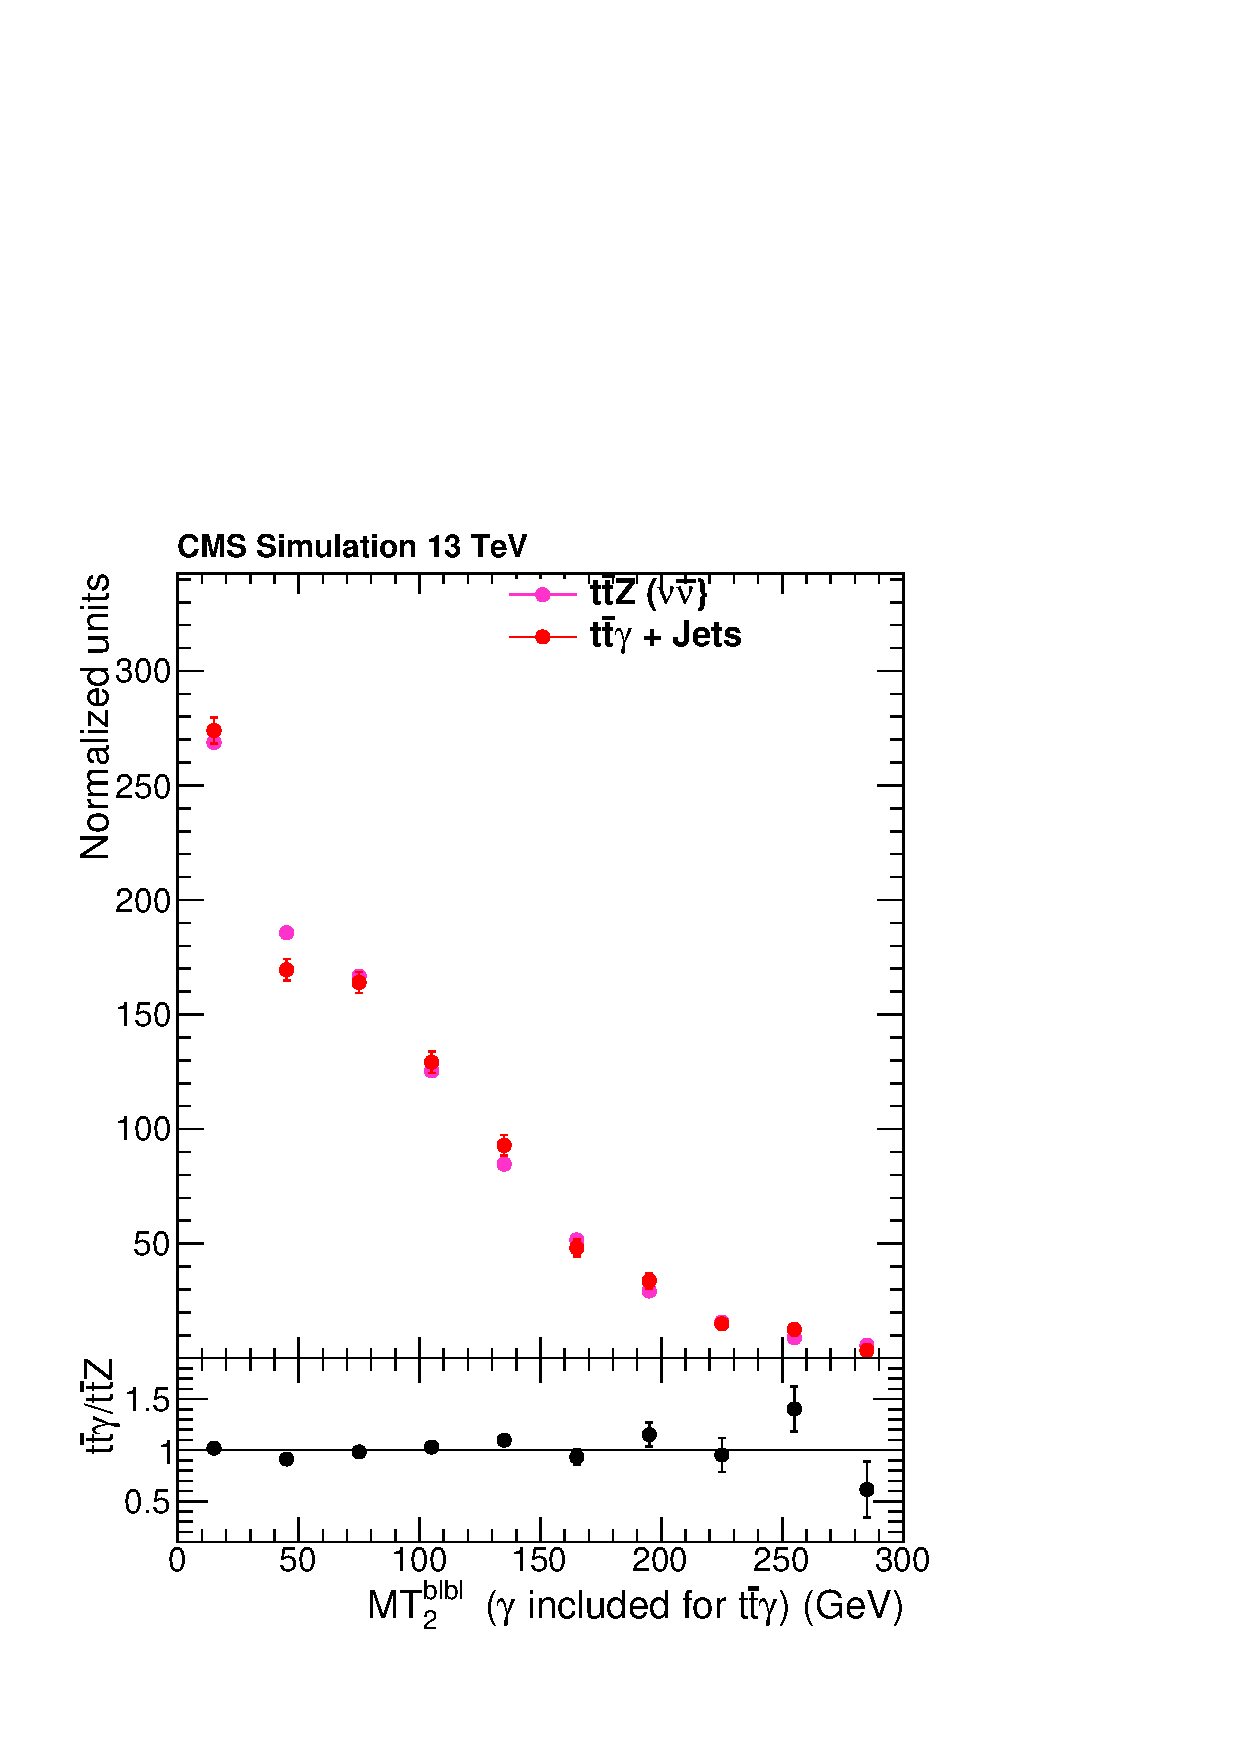
\includegraphics[width=0.45\textwidth]{figures/TTG_gen/reweighted/all_normalized/etaGamma25-ptGamma30/mt2blbl_photonIncluded.pdf}}
      \subfloat[]{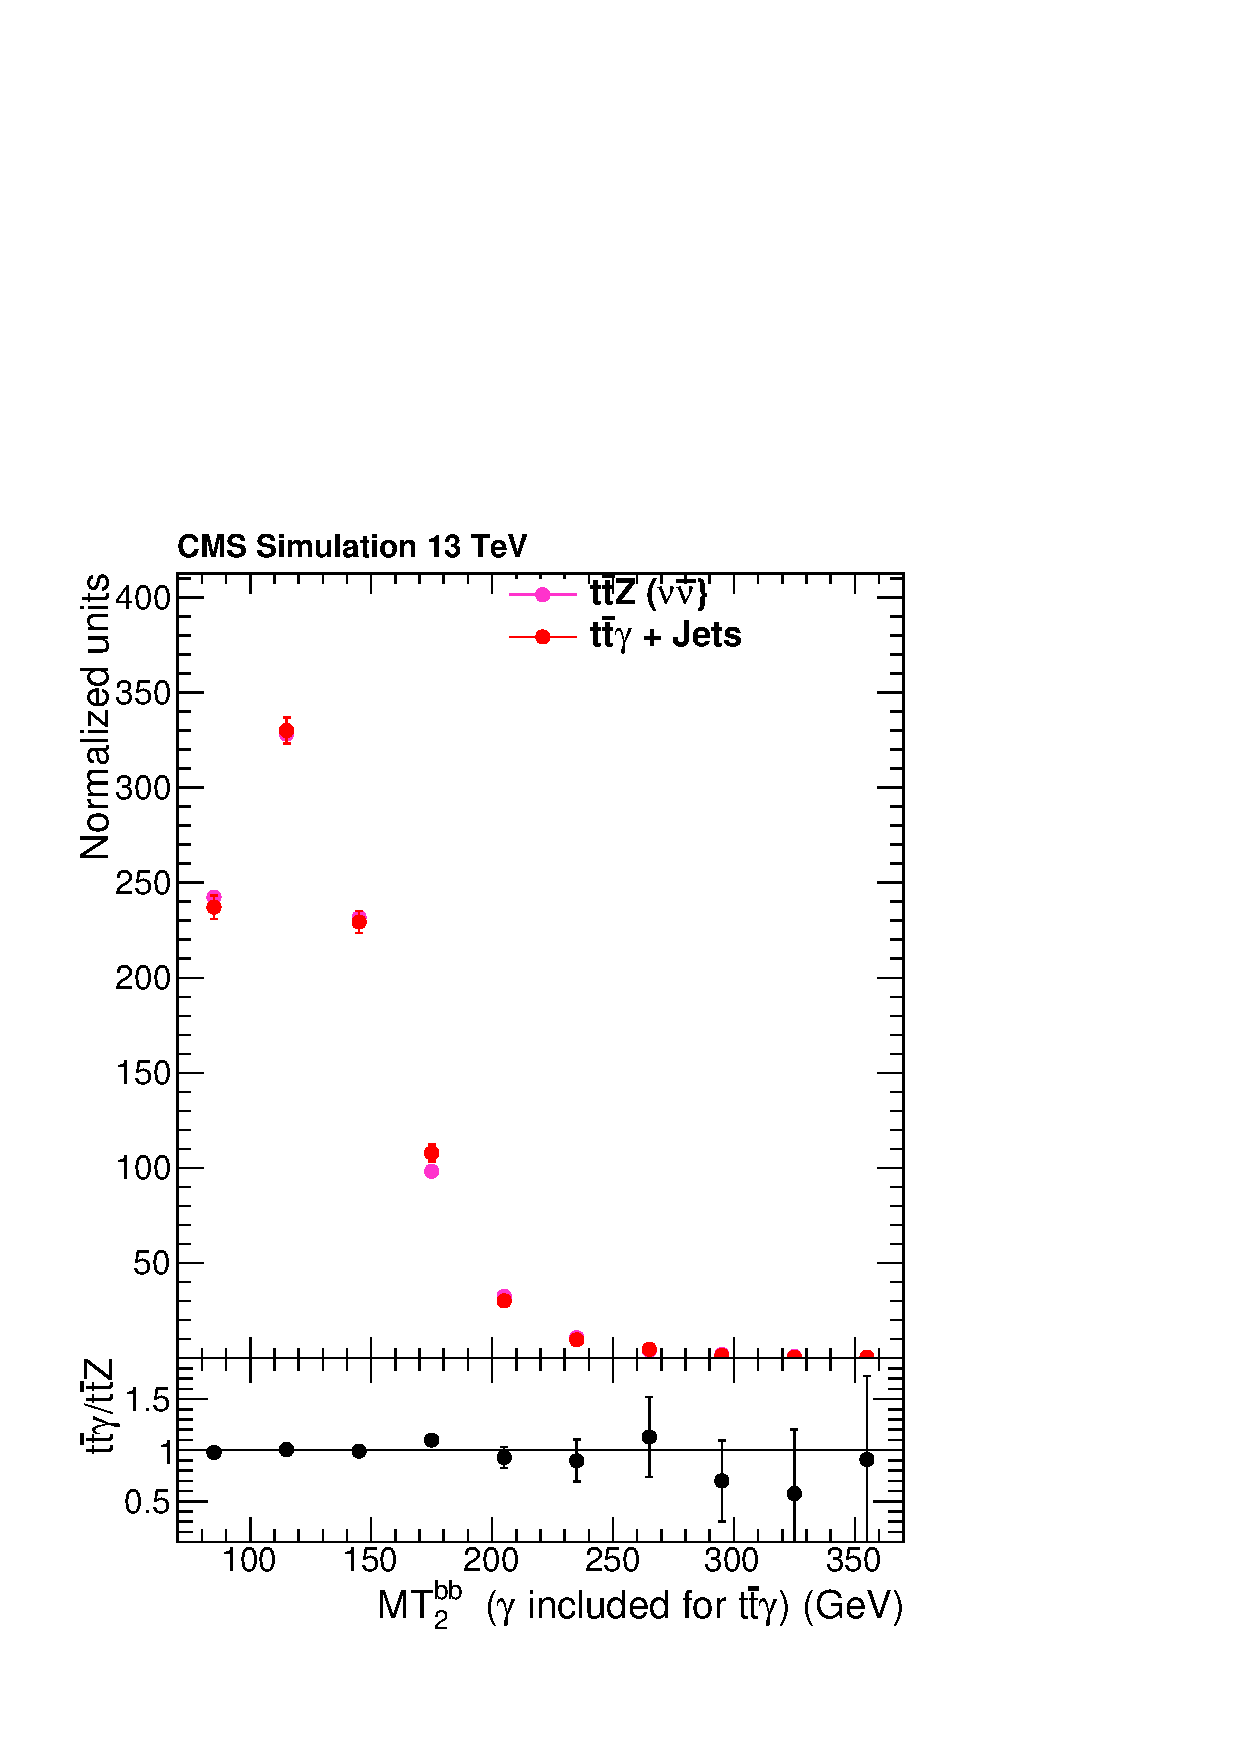
\includegraphics[width=0.45\textwidth]{figures/TTG_gen/reweighted/all_normalized/etaGamma25-ptGamma30/mt2bb_photonIncluded.pdf}}
      \caption{Generator-level comparison of $t\bar{t}\gamma$ (with photon treated as additional \met) with $t\bar{t}Z$ for the \met, \mtll, \mtlblb and \mtbb variables}
      \label{fig:ttgGen}
    \end{figure}

    In order to select a pure $t\bar{t}\gamma$ sample which is closely related to the control and signal regions of our main analysis, we use similar selections but add a photon with $\pt > 30$ \GeV falling within $|\eta| < 2.5$.
    The missing energy cuts are now replaced by \metPhoton and \metSigPhoton which are the photon-estimated variants of \met and \metSig. In order to reduce contributions of $Z\gamma$ events, the $Z$-mass window cut
    is also applied on the invariant mass $m(ll\gamma)$ of the dilepton plus gamma system, as illustrated in Figure~\ref{fig:llg}. Furthermore, photons are required to have $\Delta R(\gamma, l) > 0.3$ and $\Delta R(\gamma, j) > 0.3$, of which the latter
    is used to reject photons which are constructed as jets.
    \begin{table}
  \center
  \small
  \begin{tabular}{c|c}
                     & photons         \\
     \hline
     \pt             & $> 30\GeV$    \\    
     $|\eta|$        & $< 2.5$         \\   
     identification  & cut-based tight id  \\
  \end{tabular}
  \caption{Photon selection criteria}
  \label{photonSelection}
\end{table}


    Figure~\ref{fig:ttg_met} shows the \metPhoton before requiring the $\metPhoton > 80 \GeV$ requirement and \metSigPhoton before requiring $\metSigPhoton > 5$. The distributions of
    the photon-estimated \mtll, \mtlblb and \mtbb variables before applying the \met and \metSigPhoton requirements is shown in Figure~\ref{fig:ttg_mt2}.
    Figures~\ref{fig:ttg_mt2ll},~\ref{fig:ttg_mt2blbl} and~\ref{fig:ttg_mt2bb} show these variables after \met, \metSig and $\Delta\phi(\met, j)$ cuts, both before and after subtraction of the residual backgrounds.
    Based on the level of agreement we assign a 20\% uncertainty from the \mtll shape of TTZ. 
    
    % Data plots
    \begin{figure}
      \centering
      \subfloat[before $m(ll\gamma)$ cut]{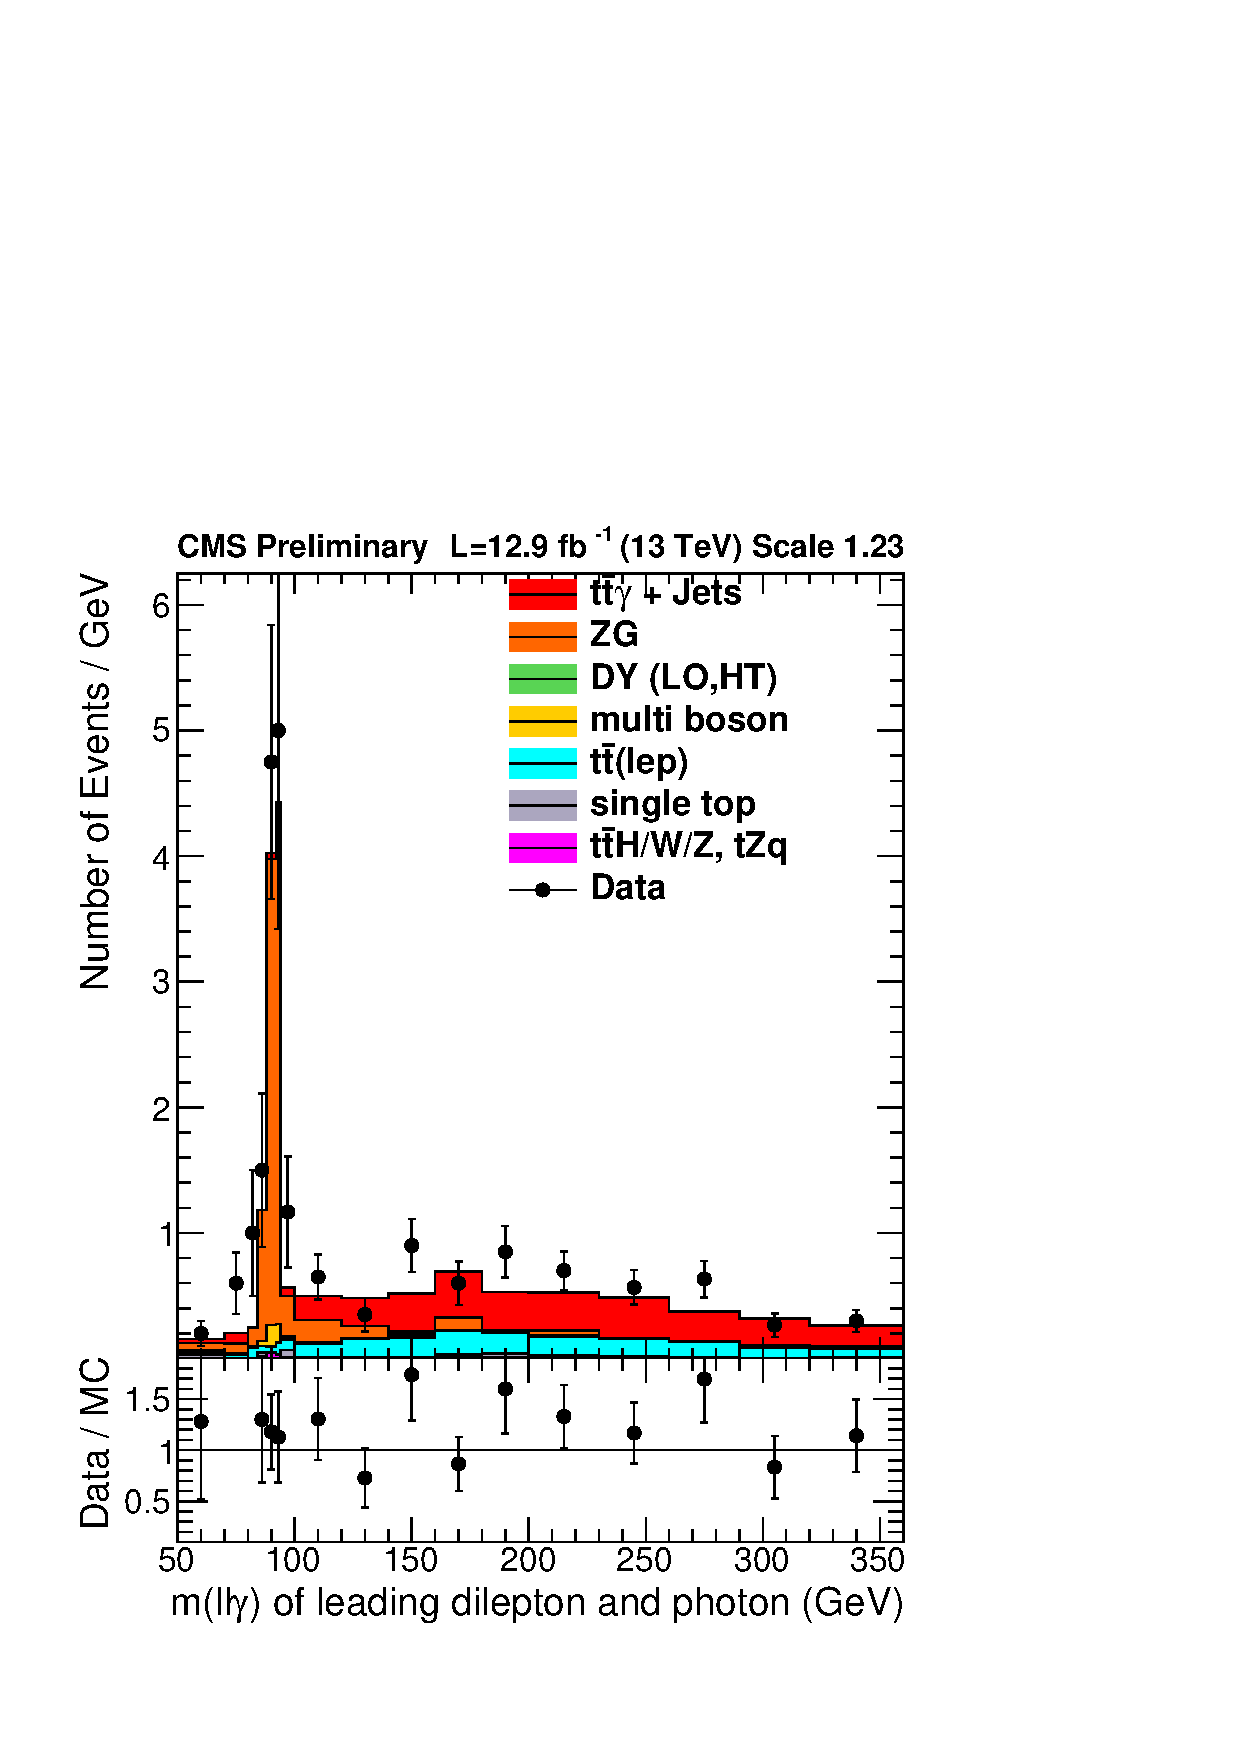
\includegraphics[width=0.45\textwidth]{figures/TTG/all/njet2-photon30-gJetdR-gLepdR-btagM/dlg_mass.pdf}}
      \subfloat[after $m(ll\gamma)$ cut]{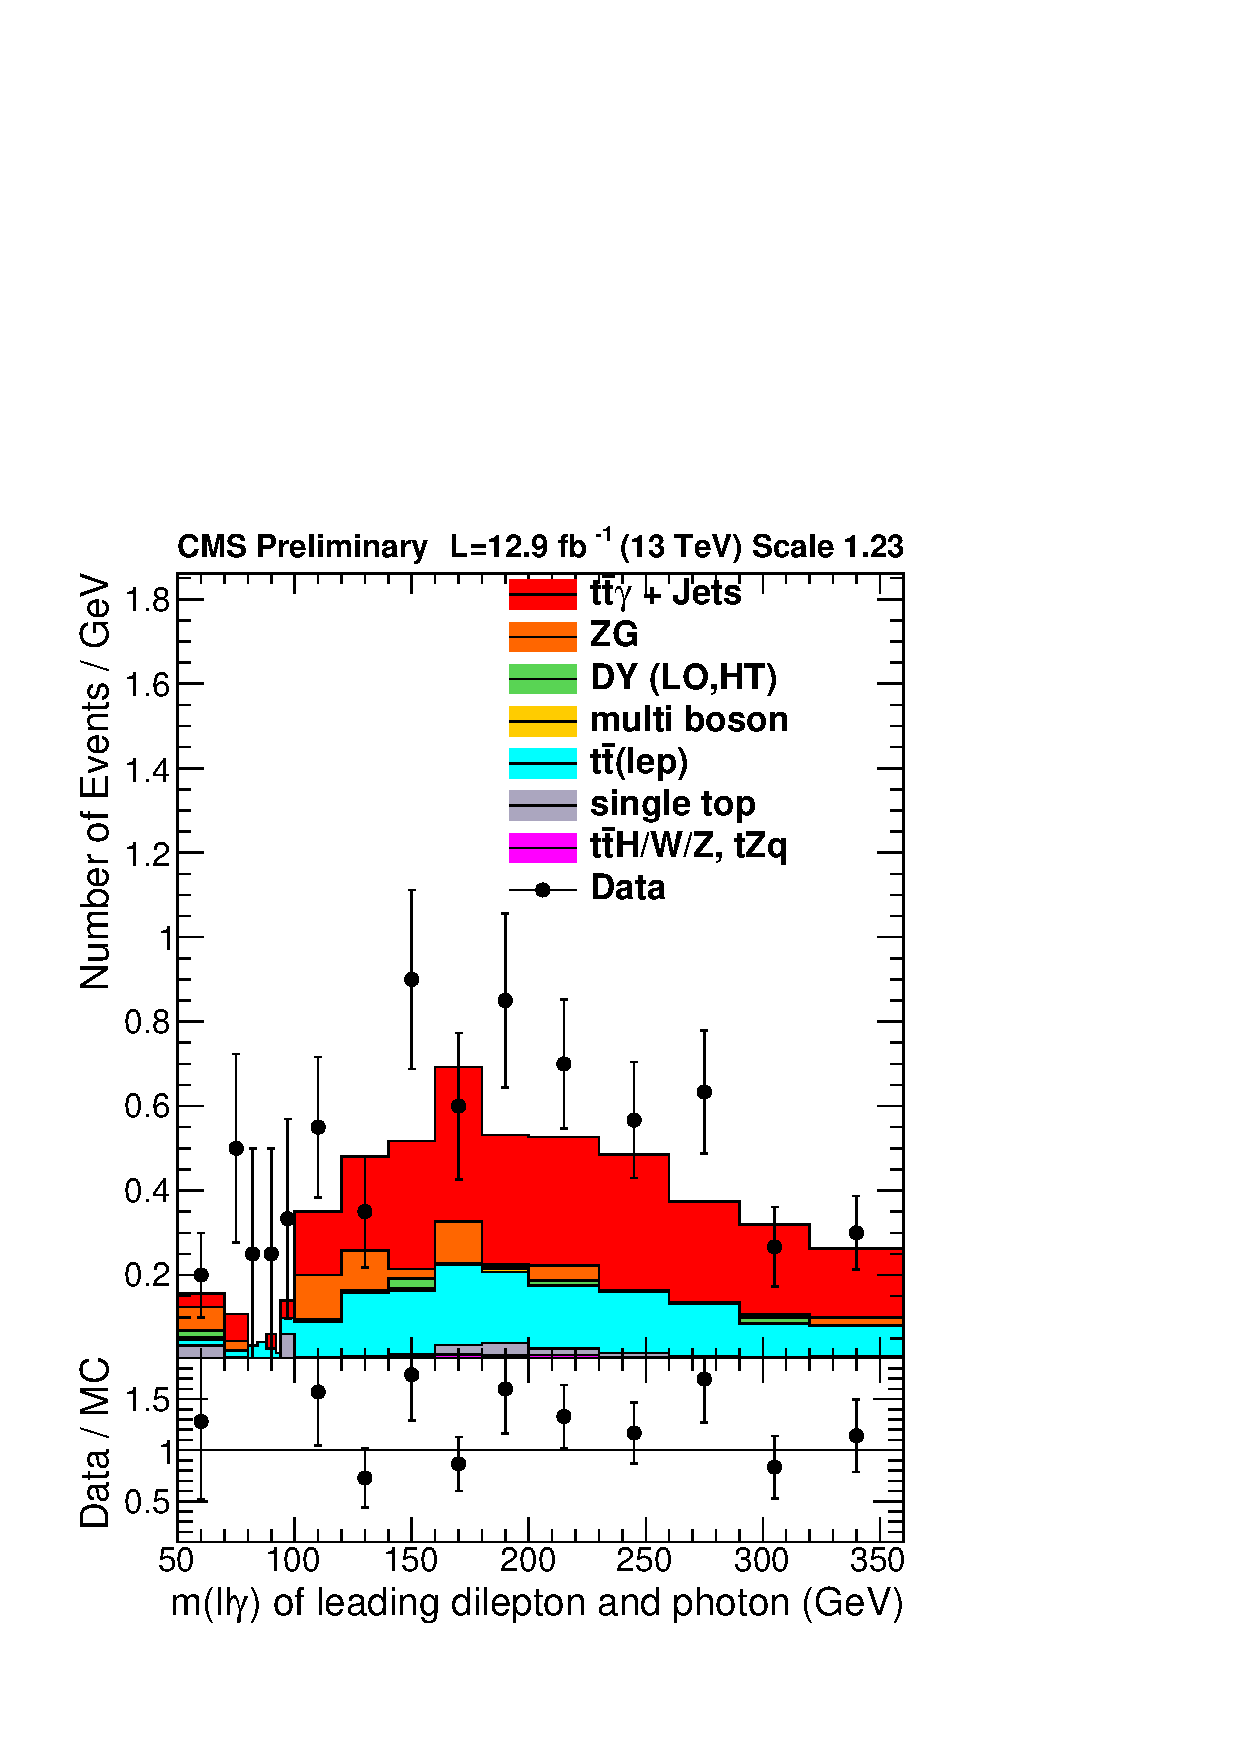
\includegraphics[width=0.45\textwidth]{figures/TTG/all/njet2-photon30-llgNoZ-gJetdR-gLepdR-btagM/dlg_mass.pdf}}
      \caption{Requiring a $Z$ window on $m(ll\gamma)$ in the same-flavour channels removes most of the $Z\gamma$ background. Given the sharp $Z$ peak in combination with a low-statistics tail, a dynamic binning
      is used for these plots, each bin showing the average number of events per \GeV for its $m(ll\gamma)$ range.}
      \label{fig:llg}
    \end{figure}

    \begin{figure}
      \centering
      \subfloat[\metPhoton]{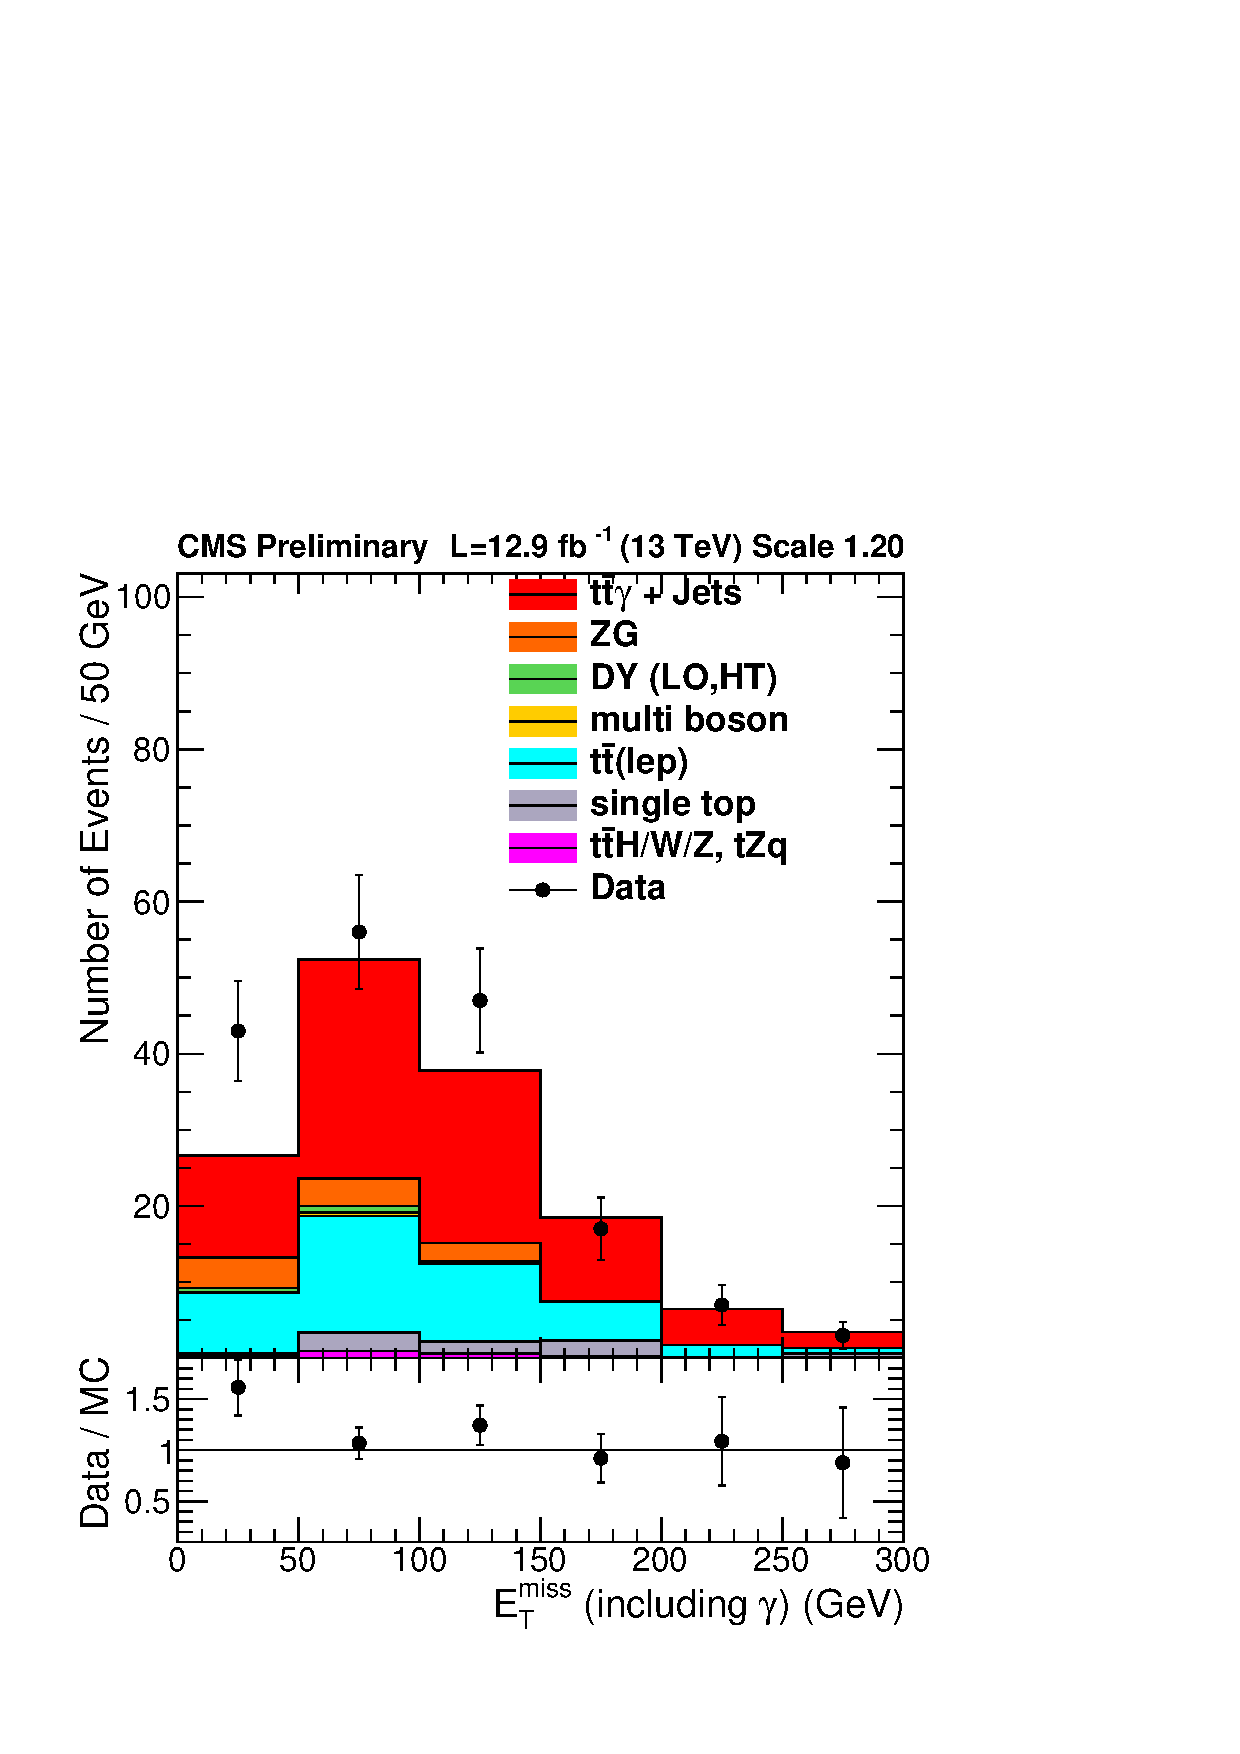
\includegraphics[width=0.45\textwidth]{figures/TTG/all/njet2-photon30-llgNoZ-gJetdR-gLepdR-btagM-mll20/met_pt_photonEstimated.pdf}}
      \subfloat[\metSigPhoton]{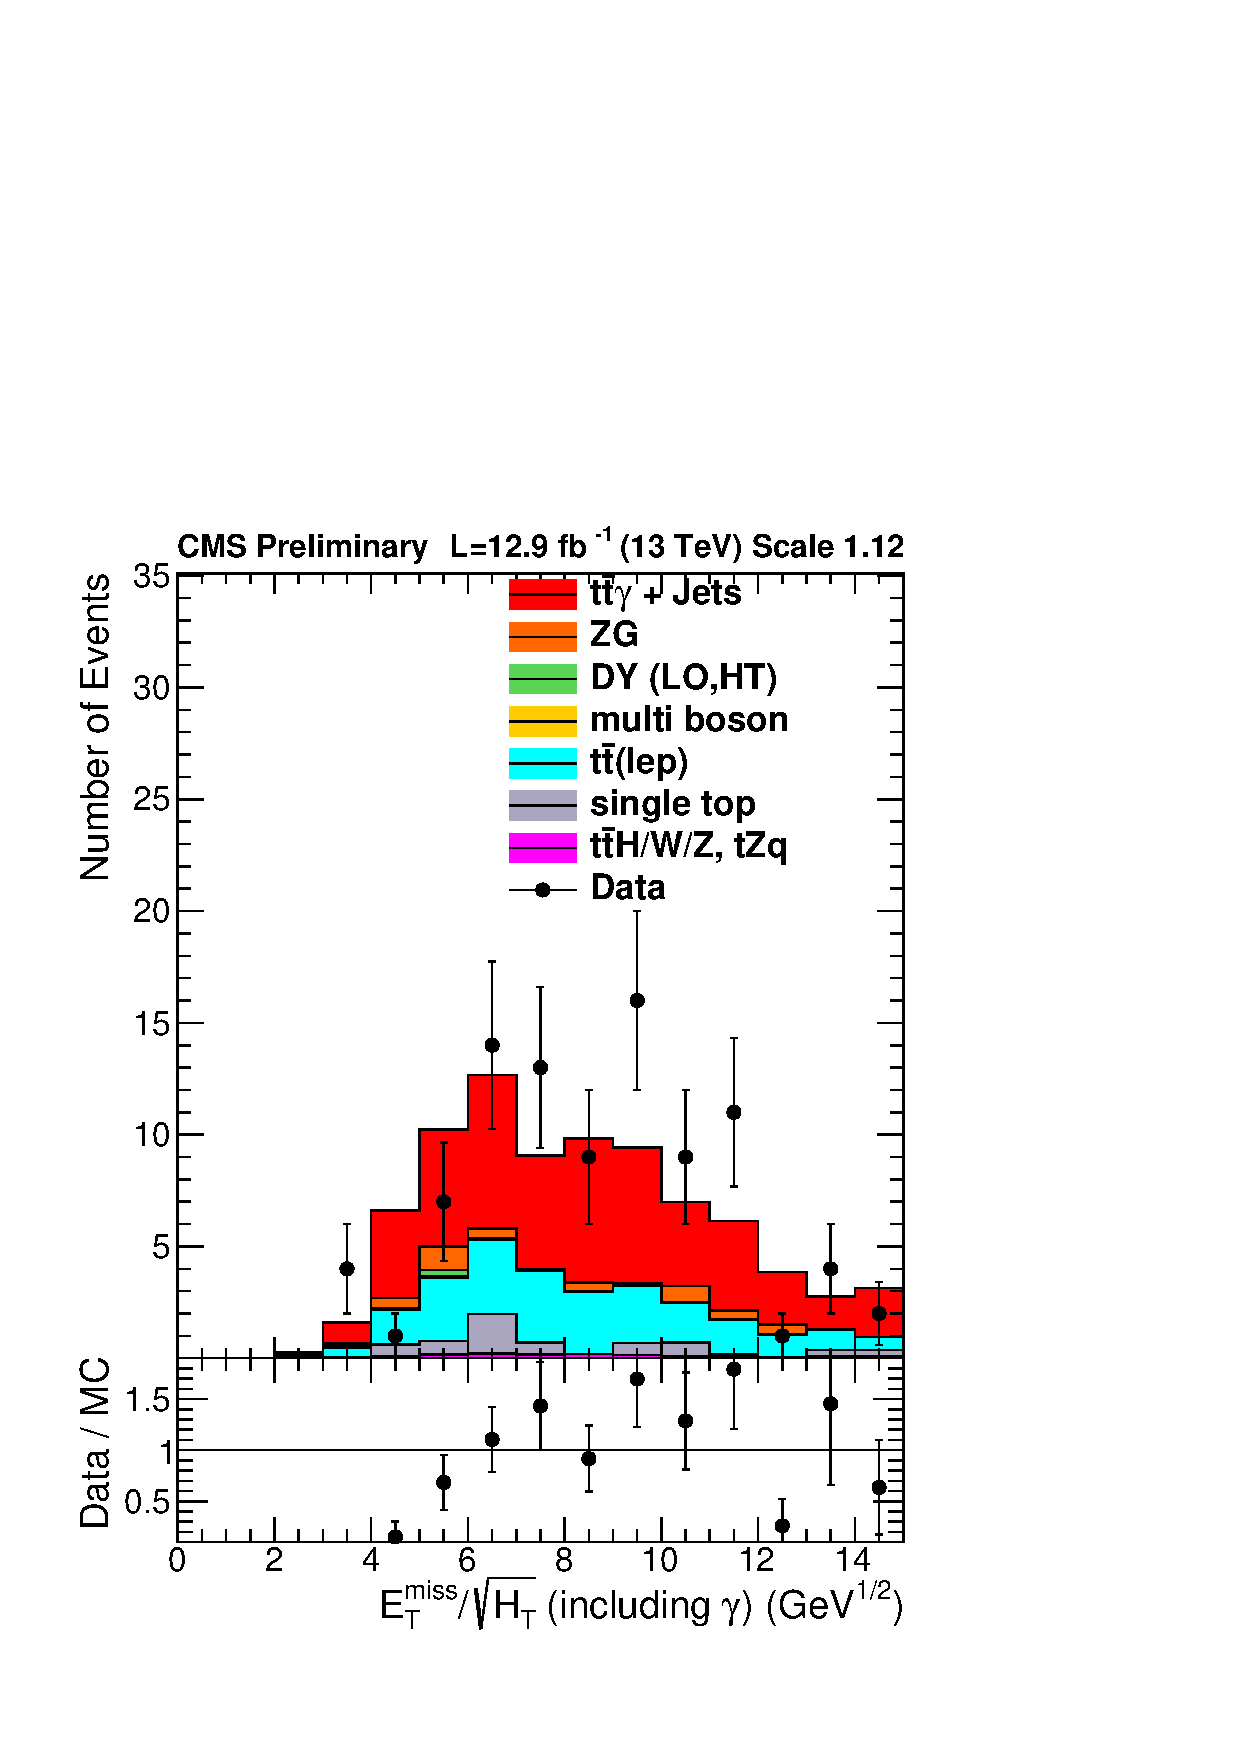
\includegraphics[width=0.45\textwidth]{figures/TTG/all/njet2-photon30-llgNoZ-gJetdR-gLepdR-btagM-mll20-met80/metSig_photonEstimated.pdf}}
      \caption{Distribution of \metPhoton and \metSigPhoton with photon \pt included in the \met calculation, before cutting on them}
      \label{fig:ttg_met}
    \end{figure}

    \begin{figure}
      \centering
      \subfloat[\mtll]{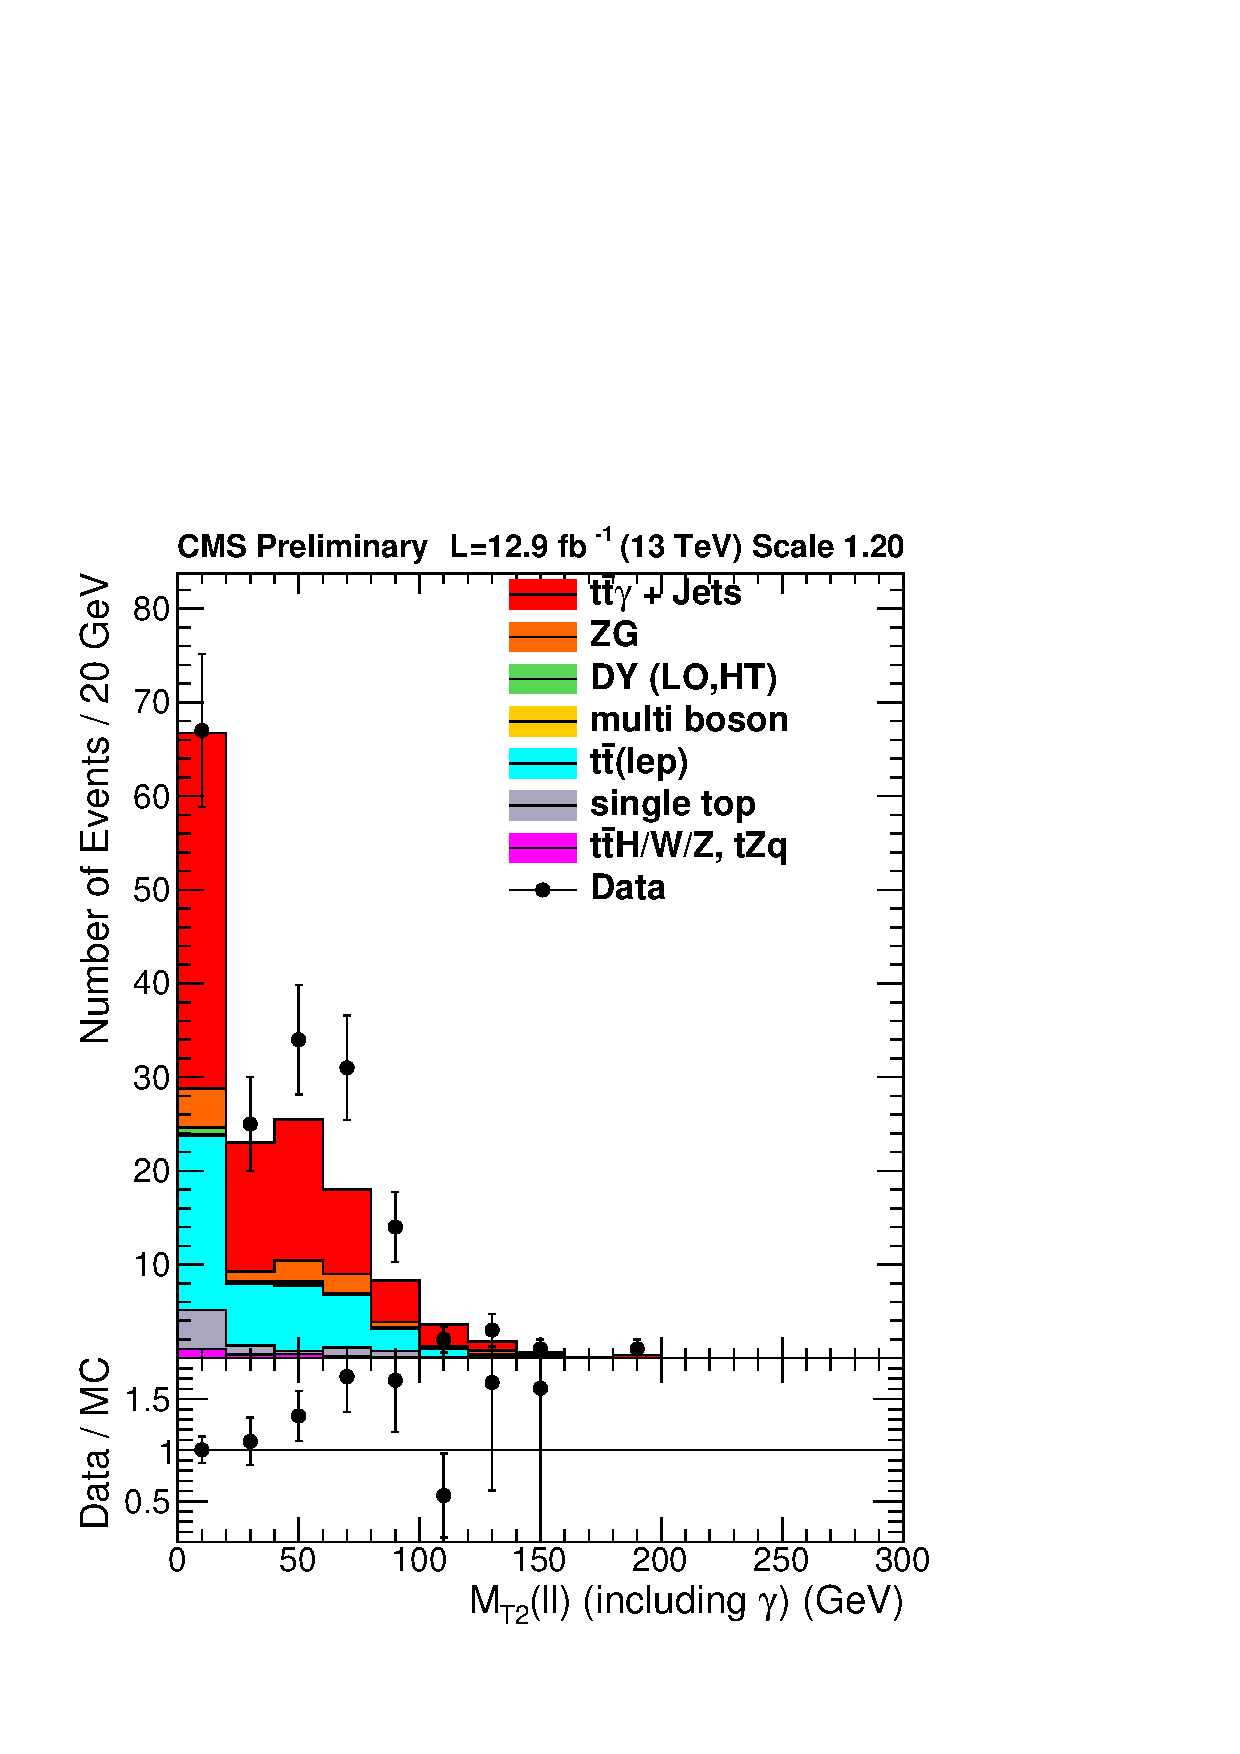
\includegraphics[width=0.32\textwidth]{figures/TTG/all/njet2-photon30-llgNoZ-gJetdR-gLepdR-btagM-mll20/dl_mt2ll_photonEstimated.pdf}}
      \subfloat[\mtlblb]{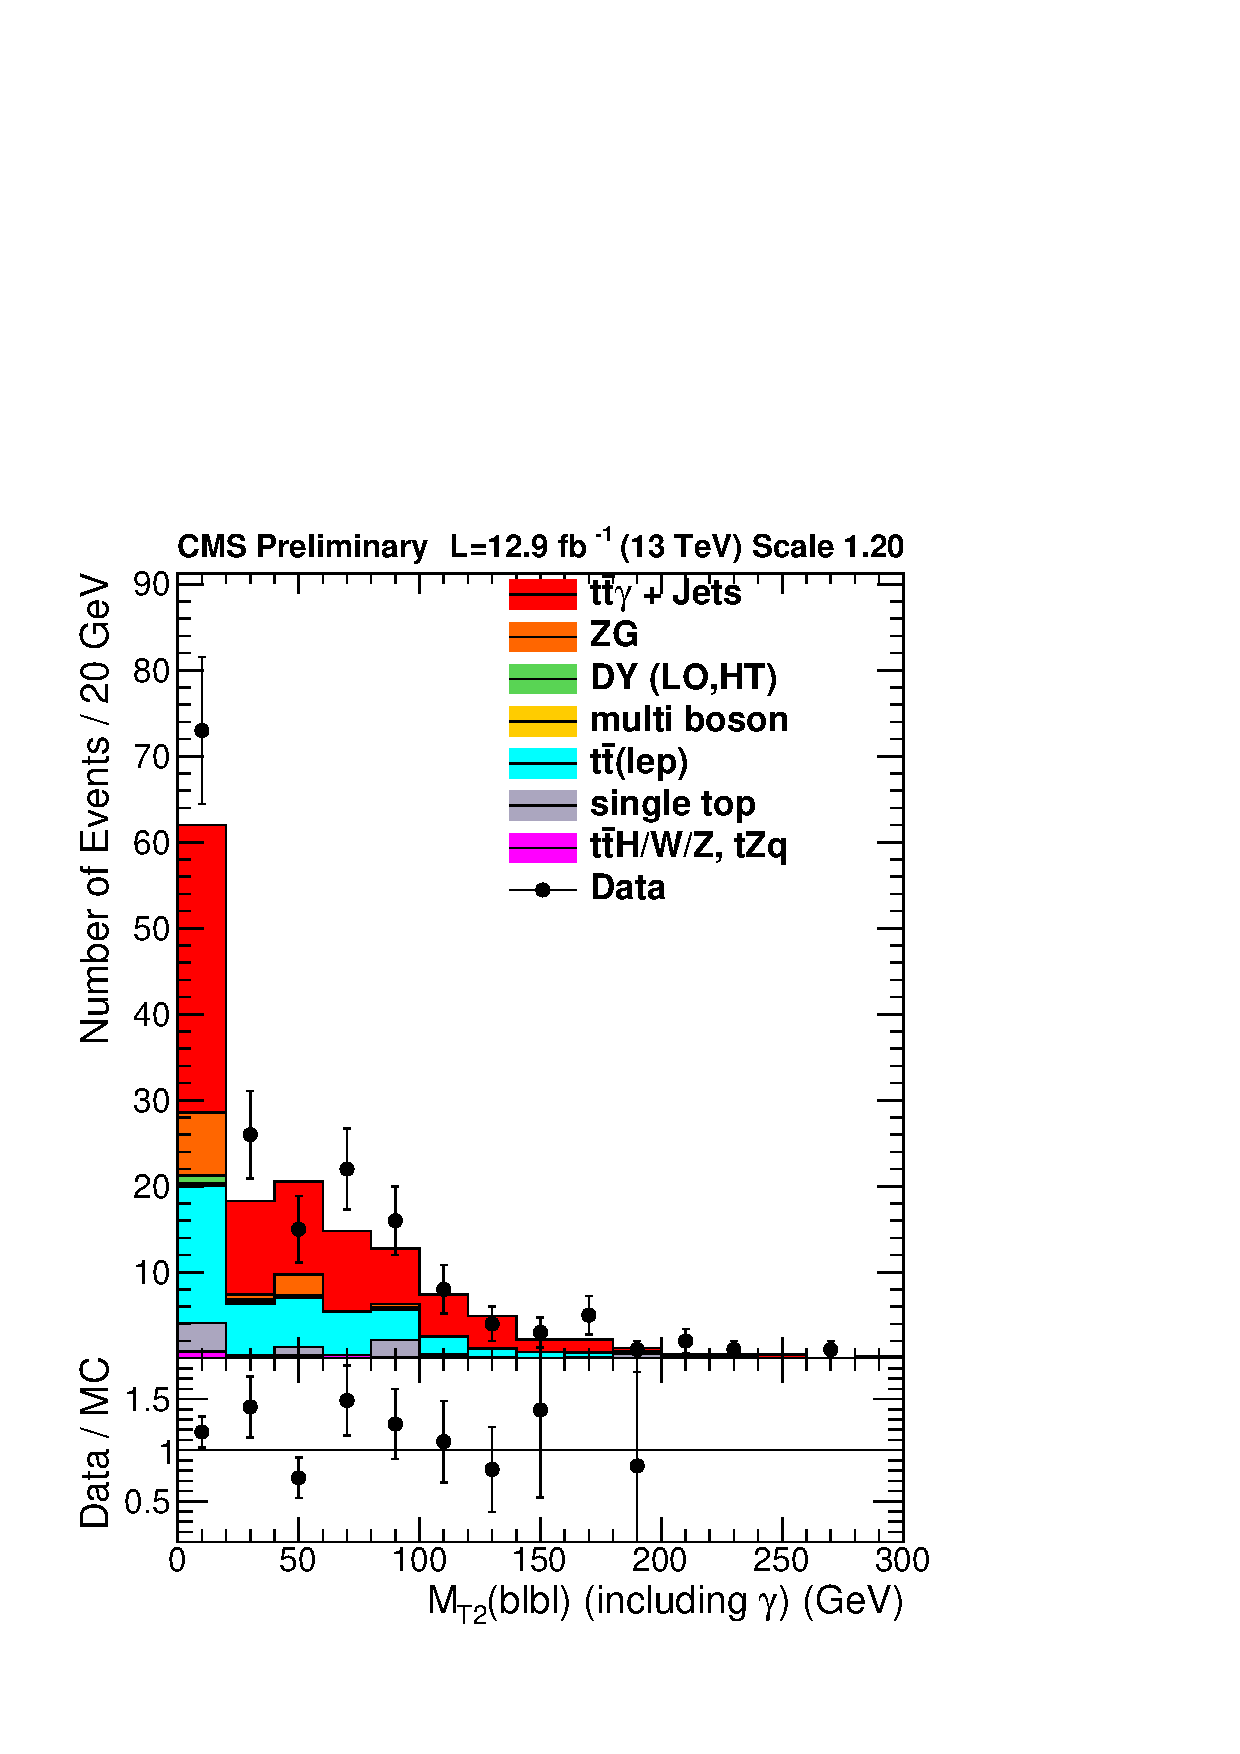
\includegraphics[width=0.32\textwidth]{figures/TTG/all/njet2-photon30-llgNoZ-gJetdR-gLepdR-btagM-mll20/dl_mt2blbl_photonEstimated.pdf}}
      \subfloat[\mtbb]{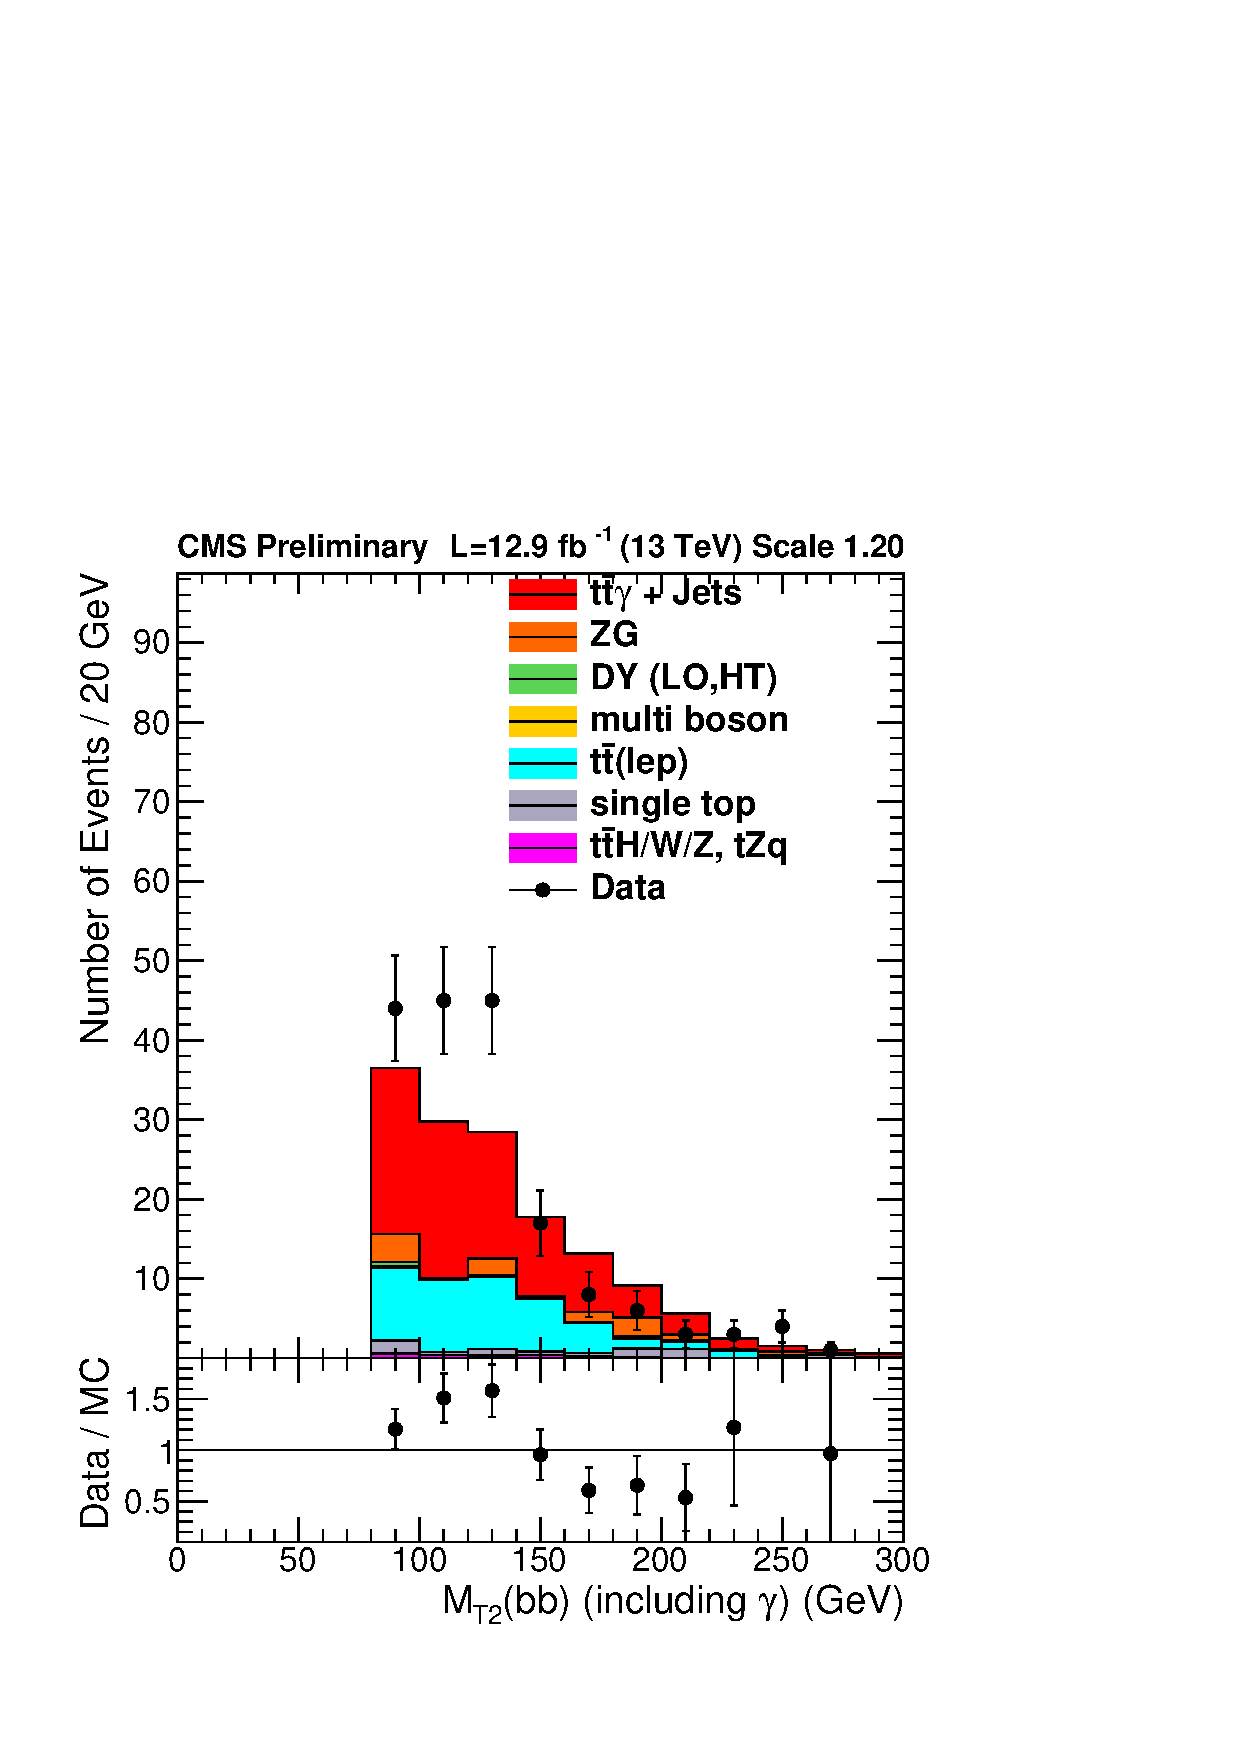
\includegraphics[width=0.32\textwidth]{figures/TTG/all/njet2-photon30-llgNoZ-gJetdR-gLepdR-btagM-mll20/dl_mt2bb_photonEstimated.pdf}}
      \caption{Distribution of \mtll, \mtlblb and \mtbb using the photon-estimated \metPhoton}
      \label{fig:ttg_mt2}
    \end{figure}

    \begin{figure}
      \centering
      \subfloat[other MC included]{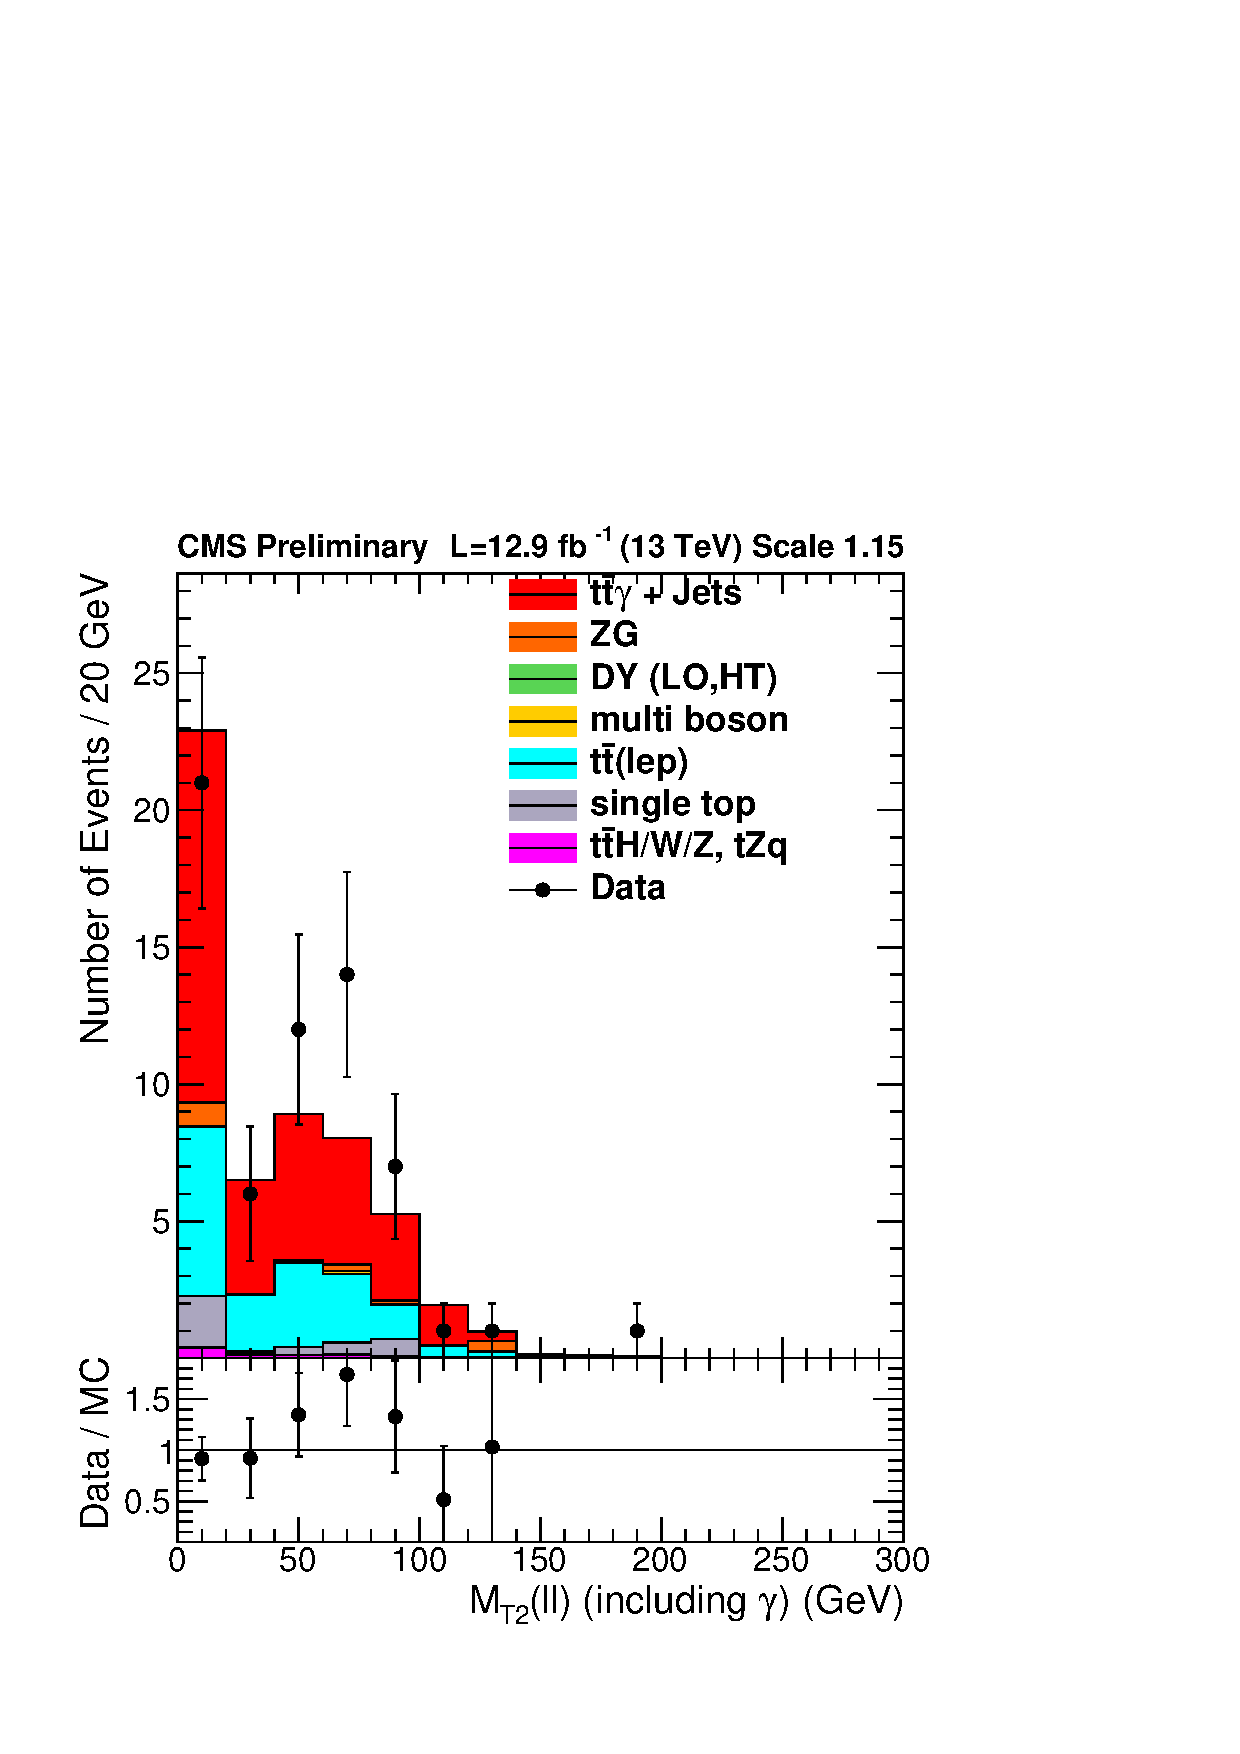
\includegraphics[width=0.45\textwidth]{figures/TTG/all/njet2-photon30-llgNoZ-gJetdR-gLepdR-btagM-mll20-met80-metSig5-dPhiJet0-dPhiJet1/dl_mt2ll_photonEstimated.pdf}}
      \subfloat[other MC subtracted]{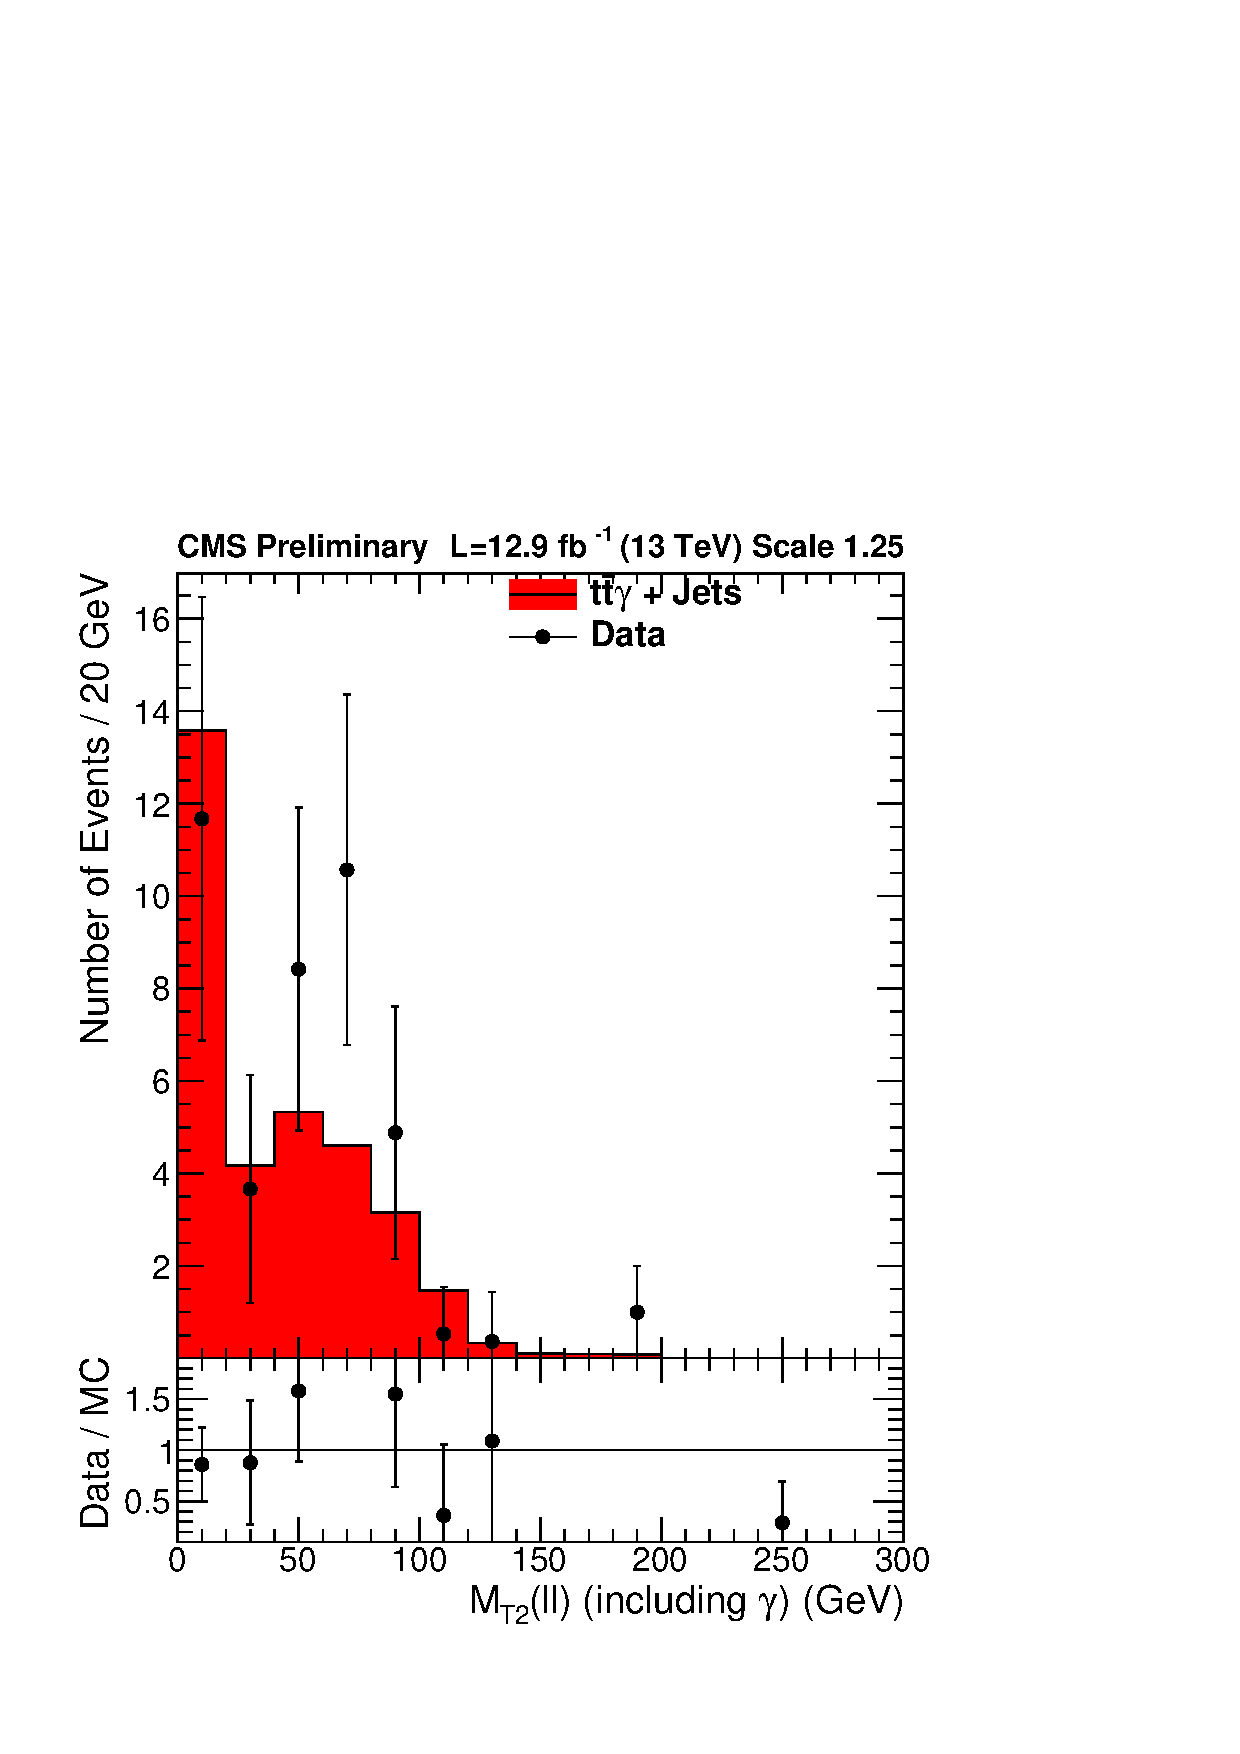
\includegraphics[width=0.45\textwidth]{figures/TTG_subtracted/all/njet2-photon30-llgNoZ-gJetdR-gLepdR-btagM-mll20-met80-metSig5-dPhiJet0-dPhiJet1/dl_mt2ll_photonEstimated.pdf}}
      \caption{Distribution of \mtll using the photon-estimated \metPhoton (after \met cuts)}
      \label{fig:ttg_mt2ll}
    \end{figure}

    \begin{figure}
      \centering
      \subfloat[other MC included]{\includegraphics[width=0.45\textwidth]{figures/TTG/all/njet2-photon30-llgNoZ-gJetdR-gLepdR-btagM-mll20-met80-metSig5-dPhiJet0-dPhiJet1/dl_mt2blbl_photonEstimated.pdf}}
      \subfloat[other MC subtracted]{\includegraphics[width=0.45\textwidth]{figures/TTG_subtracted/all/njet2-photon30-llgNoZ-gJetdR-gLepdR-btagM-mll20-met80-metSig5-dPhiJet0-dPhiJet1/dl_mt2blbl_photonEstimated.pdf}}
      \caption{Distribution of \mtlblb using the photon-estimated \metPhoton (after \met cuts)}
      \label{fig:ttg_mt2blbl}
    \end{figure}

    \begin{figure}
      \centering
      \subfloat[other MC included]{\includegraphics[width=0.45\textwidth]{figures/TTG/all/njet2-photon30-llgNoZ-gJetdR-gLepdR-btagM-mll20-met80-metSig5-dPhiJet0-dPhiJet1/dl_mt2bb_photonEstimated.pdf}}
      \subfloat[other MC subtracted]{\includegraphics[width=0.45\textwidth]{figures/TTG_subtracted/all/njet2-photon30-llgNoZ-gJetdR-gLepdR-btagM-mll20-met80-metSig5-dPhiJet0-dPhiJet1/dl_mt2bb_photonEstimated.pdf}}
      \caption{Distribution of \mtbb using the photon-estimated \metPhoton (after \met cuts)}
      \label{fig:ttg_mt2bb}
    \end{figure}

\subsection{Rare backgrounds}
Rare backgrounds whose contribution is negligible in all search regions are \ttbar production in association with a Higgs boson and triple gauge boson background.
Those are taken from simulation and assigned an uncertainty of 50\%.

\section{Systematic uncertainties}
\label{sec:systematics}

Besides the systematics related to the background estimation techniques discussed in Sec.~\ref{sec:background_estimations} we following the ICHEP recommendations~\cite{twiki:sys} for signal systematics and the POG recommended experimental uncertainties.

%%% Uncorrelated point by point MC statistical uncertainty

Specifically, the jet energy scale (JES) is varied within uncertainty~\cite{Chatrchyan:2011ds} as a function of jet \pt and $\eta$, and
these changes are propagated to all observables, including \ETmiss. The \ETmiss observable is moreover subject to uncertainties from the 
unclustered energy which is varied within uncertainties.

The simulated efficiencies for the identification of b-quark jets and for the misidentification of c-quark,
light-quark or gluon jets need to be corrected for with scale factors and their respective uncertainties~\cite{CMS-PAS-BTV-15-001} are evaluated using method 1a~\cite{twiki:btagSF}.

Uncertainties for the efficiency of lepton reconstruction and identification according to the ICHEP data set are handled in the same way. We consider
lepton-ID efficiencies (electrons and muons separately) that were derived for our particular lepton definition. Moreover, we correct the simulation based
on studies of the HIP effect (heavily ionizing particle) that accounts for a dynamic inefficiency of the silicon strip tracker and hence a reduction in tracking efficiency
as a function of instantaneous luminosity. 

To adjust the simulated PU activity to data, we perform a rewighting based on a total inelastic crossection of 69.2~mb and apply a 5\% uncertainty that we propagate to the reweighting histogram..
The luminosity is measured with the pixel cluster counting method, and the absolute luminosity scale calibration is derived from
an analysis of Van der Meer scans performed in May 2016, resulting in an uncertainty of 6.2\%~\cite{LUMI2016}

Trigger efficiencies are applied as described in Sec.\ref{sec:trigger} and the corresponding bin-by-bin uncertainties are applied as systematics in a correlated way.
Uncertainties on the lepton scale factors following the POG prescriptions~\citep{twiki:eSFsys}.
When a background or signal yield is taken from a simulated sample, the statistical uncertainties are taken into account.
These uncertainties discussed so far, apply to both the background prediction and the signal yield.

Specifically for the backgrounds, the \pt distribution of the top quarks in \ttbar events have found to be softer in 8 \TeV data compared to the prediction by various simulations. 
Based on the NNLO prediction, which gives a reasonable description of the \pt spectrum in data,
a reweighting function has been introduced to alter the shape according to $\sqrt{w(t)\cdot w(\overline{t})}$ where
\begin{equation}
w(\pt) = e^{0.148-0.00129\pt}.
\end{equation}
The reweighting is applied such that it preserves the normalization of the sample, and the difference relative to the results obtained with the unweighted sample is assigned as a systematic uncertainty.

For the signals, an uncertainty on initial-state radiation (ISR) is applied, based on the number of jets which are not matched to simulated particles descending from top quarks, W,Z or Higgs bosons or SUSY particles. The event is reweighted based on the distribution of this observables but correcting for the total change in the crosssection of the respective mass point.
The factorization and renormalization scale are each changed by a factor of 0.5 and 2 and the envelope of variations on the predicted signal yield is assigned as systematic; anti-correlated variations
are not considered.
Finally, uncertainties in the signal cross section are also taken into account.

\subsection{Kinematic distributions in the pre-selection}
\label{sec:preselectionplots}
Figures~\ref{fig:jetsSys} and \ref{fig:mt2llSys} show the distributions of number of jets, medium $b$-tags and \mtll, \mtbb and \mtlblb variables including uncertainty bands from the JEC, \ETmiss uncertainties, top \pt and PU reweighting systematics.
Figure~\ref{fig:mt2bbSys} shows \mtbb and \mtlblb after selecting events with $\mtll > 100$ GeV, where scale factors for $t\bar{t}$, DY, diboson and $t\bar{t}Z$ backgrounds are applied, and their shape uncertainties
are added to the uncertainty band.

\begin{figure}
\centering
\subfloat[]{\includegraphics[width=0.45\textwidth]{figures/systematicPlots/all_log_scaled/njet2-btagM-multiIsoWP-looseLeptonVeto-mll20-met80-metSig5-dPhiJet0-dPhiJet1/njets_normalizeBinWidth.pdf}}
\subfloat[]{\includegraphics[width=0.45\textwidth]{figures/systematicPlots/all_log_scaled/njet2-btagM-multiIsoWP-looseLeptonVeto-mll20-met80-metSig5-dPhiJet0-dPhiJet1/nbtags_normalizeBinWidth.pdf}}
\caption{Number of jets and medium $b$-tags}
\label{fig:jetsSys}
\end{figure}


\begin{figure}
\centering
\subfloat[]{\includegraphics[width=0.45\textwidth]{figures/systematicPlots/all_log_scaled/njet2-btagM-multiIsoWP-looseLeptonVeto-mll20-met80-metSig5-dPhiJet0-dPhiJet1/met_pt_normalizeBinWidth.pdf}}
\subfloat[]{\includegraphics[width=0.45\textwidth]{figures/systematicPlots/all_log_scaled/njet2-btagM-multiIsoWP-looseLeptonVeto-mll20-met80-metSig5-dPhiJet0-dPhiJet1/dl_mt2ll_normalizeBinWidth.pdf}} \\
\caption{Distributions of \ETslash and \mtll after pre-selection.}
\label{fig:mt2llSys}
\end{figure}

\begin{figure}
\centering
\subfloat[]{\includegraphics[width=0.45\textwidth]{figures/systematicPlots/all_log_scaled/njet2-btagM-multiIsoWP-looseLeptonVeto-mll20-met80-metSig5-dPhiJet0-dPhiJet1-mt2ll100/dl_mt2bb_normalizeBinWidth.pdf}}
\subfloat[]{\includegraphics[width=0.45\textwidth]{figures/systematicPlots/all_log_scaled/njet2-btagM-multiIsoWP-looseLeptonVeto-mll20-met80-metSig5-dPhiJet0-dPhiJet1-mt2ll100/dl_mt2blbl_normalizeBinWidth.pdf}}
\caption{Distributions of \mtbb and \mtlblb after pre-selection and $\mtll > 100$ GeV. Scale factors are applied for the $t\bar{t}$, DY, diboson and $t\bar{t}Z$ backgrounds.}
\label{fig:mt2bbSys}
\end{figure}

\begin{table}
\centering
\begin{tabular}{l|c} 
  systematic & min-max of signal regions (\%) \\ 
  \hline 
MC statistics & 4  - 40  \\ 
pile-up & $<$ 14  \\ 
JEC & $<$ 36  \\ 
top-\pt & $<$ 3  \\ 
trigger & $<$ 1  \\ 
lepton SF & $<$ 3  \\ 
b-tag SF-b & $<$ 4  \\ 
b-tag SF-l & $<$ 5  \\ 
top background & $<$ 50  \\ 
$t\bar{t}Z$ background & $<$ 12  \\ 
multiboson background & $<$ 10  \\ 
$t\bar{t}X$ (excl. $t\bar{t}Z$) background & $<$ 8  \\ 
DY background & $<$ 12  \\ 
\end{tabular} 

\caption{Minimal and maximal relative errors for the systematics over all signal regions (all channels combined). Numbers are given relative to the total background contribution per signal region.}
\end{table}

\section{Results}

  For each of the signal regions, the total expectation  and observed yields are shown in Tables~\ref{table:yield_EMu},~\ref{table:yield_SF} and ~\ref{table:yield_all} for respectively the $e\mu$ channel, same-flavor channels
  and, moreover, for all the channels combined. When calculating the total expect yields, the $t\bar{t}$, DY, diboson and $t\bar{t}Z$ scale factors as well as their uncertainties are taken into account. 
  The uncertainties related to MC statistics, pile-up, jet energy scale, top-$\pt$ reweighting, trigger efficiencies, lepton identification and isolation scale factors, $b$-tagging scale factors
  and the different background components are also included.
  The observed yields and its statistically are also visually presented in Figures~\ref{fig:signalRegions-emu},~\ref{fig:signalRegions-sf} and~\ref{fig:signalRegions-all} where, additionally, three
  signal mass configurations are overlaid. The uncertainty band includes the MC statistics, pile-up, jet energy scale, top-$\pt$ reweighting, trigger efficiencies, lepton identification and isolation scale factors, $b$-tagging scale factors
  uncertainties.
  The observation is in agreement with the prediction within uncertainties.

  \begin{sidewaystable}
    \centering
    \setlength{\tabcolsep}{4pt}
    \footnotesize
    \begin{tabular}{l|cc|cccccccc|ccccc} 
  \rotatebox[origin=c]{50}{signal region} & \rotatebox[origin=c]{50}{observed} & \rotatebox[origin=c]{50}{expected}&\rotatebox[origin=c]{50}{MC stat}&\rotatebox[origin=c]{50}{PU}&\rotatebox[origin=c]{50}{JEC}&\rotatebox[origin=c]{50}{top-\pt}&\rotatebox[origin=c]{50}{trigger}&\rotatebox[origin=c]{50}{lepton SF}&\rotatebox[origin=c]{50}{b-tag SF-b}&\rotatebox[origin=c]{50}{b-tag SF-l}&\rotatebox[origin=c]{50}{TTJets}&\rotatebox[origin=c]{50}{TTZ}&\rotatebox[origin=c]{50}{multiBoson}&\rotatebox[origin=c]{50}{TTXNoZ}&\rotatebox[origin=c]{50}{DY} \\ 
  \hline 
 $0$  & 40 & 27.80 & 1.35 & 0.77 & 1.06 & 0.46 & 0.05 & 0.04 & 0.05 & 0.01 & 26.78 $\pm$ 13.39 & 0.17 $\pm$ 0.04 & 0.34 $\pm$ 0.09 & 0.18 $\pm$ 0.05 & 0.0 $\pm$ 0.00 \\ 
 $1$  & 3 & 1.00 & 0.25 & 0.08 & 0.05 & 0.01 & 0.01 & 0.01 & 0.01 & 0.01 & 0.98 $\pm$ 0.50 & 0.02 $\pm$ 0.01 & 0.0 $\pm$ 0.00 & 0.0 $\pm$ 0.00 & 0.0 $\pm$ 0.00 \\ 
 $2$  & 18 & 13.24 & 0.89 & 0.21 & 0.06 & 0.14 & 0.02 & 0.02 & 0.02 & 0.02 & 12.42 $\pm$ 6.21 & 0.39 $\pm$ 0.08 & 0.11 $\pm$ 0.03 & 0.21 $\pm$ 0.06 & 0.0 $\pm$ 0.00 \\ 
 $3$  & 1 & 1.13 & 0.19 & 0.03 & 0.07 & 0.01 & 0.01 & 0.01 & 0.02 & 0.01 & 0.85 $\pm$ 0.43 & 0.05 $\pm$ 0.02 & 0.05 $\pm$ 0.02 & 0.13 $\pm$ 0.04 & 0.0 $\pm$ 0.00 \\ 
 $4$  & 0 & 0.06 & 0.03 & 0.01 & 0.01 & 0.01 & 0.01 & 0.01 & 0.01 & 0.00 & 0.03 $\pm$ 0.02 & 0.02 $\pm$ 0.01 & 0.0 $\pm$ 0.00 & 0.0 $\pm$ 0.01 & 0.0 $\pm$ 0.00 \\ 
 $5$  & 0 & 0.90 & 0.44 & 0.02 & 0.04 & 0.01 & 0.01 & 0.01 & 0.01 & 0.01 & 0.78 $\pm$ 0.39 & 0.1 $\pm$ 0.02 & 0.0 $\pm$ 0.00 & 0.03 $\pm$ 0.01 & 0.0 $\pm$ 0.00 \\ 
 $6$  & 0 & 0.12 & 0.07 & 0.01 & 0.01 & 0.01 & 0.01 & 0.01 & 0.01 & 0.01 & 0.1 $\pm$ 0.06 & 0.02 $\pm$ 0.01 & 0.0 $\pm$ 0.00 & 0.0 $\pm$ 0.00 & 0.0 $\pm$ 0.00 \\ 
 $7$  & 0 & 0.01 & 0.02 & 0.01 & 0.01 & 0.01 & 0.00 & 0.01 & 0.01 & 0.00 & 0.01 $\pm$ 0.01 & 0.0 $\pm$ 0.01 & 0.0 $\pm$ 0.00 & 0.0 $\pm$ 0.01 & 0.0 $\pm$ 0.00 \\ 
 $8$  & 0 & 0.48 & 0.12 & 0.01 & 0.02 & 0.02 & 0.01 & 0.01 & 0.01 & 0.01 & 0.27 $\pm$ 0.14 & 0.15 $\pm$ 0.03 & 0.0 $\pm$ 0.00 & 0.07 $\pm$ 0.02 & 0.0 $\pm$ 0.00 \\ 
 $9$  & 0 & 0.05 & 0.03 & 0.01 & 0.02 & 0.00 & 0.01 & 0.01 & 0.01 & 0.00 & 0.0 $\pm$ 0.00 & 0.01 $\pm$ 0.01 & 0.0 $\pm$ 0.00 & 0.04 $\pm$ 0.01 & 0.0 $\pm$ 0.00 \\ 
 $10$  & 1 & 0.18 & 0.07 & 0.02 & 0.02 & 0.01 & 0.01 & 0.01 & 0.01 & 0.01 & 0.04 $\pm$ 0.02 & 0.11 $\pm$ 0.03 & 0.01 $\pm$ 0.01 & 0.01 $\pm$ 0.01 & 0.0 $\pm$ 0.00 \\ 
 $11$  & 0 & 0.24 & 0.08 & 0.01 & 0.01 & 0.01 & 0.01 & 0.01 & 0.01 & 0.01 & 0.07 $\pm$ 0.04 & 0.11 $\pm$ 0.03 & 0.0 $\pm$ 0.00 & 0.07 $\pm$ 0.02 & 0.0 $\pm$ 0.00 \\ 
 $12$  & 0 & 0.05 & 0.02 & 0.01 & 0.01 & 0.00 & 0.01 & 0.01 & 0.01 & 0.00 & 0.0 $\pm$ 0.00 & 0.04 $\pm$ 0.01 & 0.0 $\pm$ 0.00 & 0.0 $\pm$ 0.01 & 0.0 $\pm$ 0.00 \\ 
\end{tabular} 

    \caption{Yields and uncertainties for the total background in each of the signal regions for the $e\mu$ channel. Scale factors are applied for the $t\bar{t}$, DY, diboson and $t\bar{t}Z$ backgrounds.}
    \label{table:yield_EMu}
  \end{sidewaystable}

  \begin{sidewaystable}
    \centering
    \footnotesize
    \setlength{\tabcolsep}{4pt}
    \begin{tabular}{l|cc|cccccccc|ccccc} 
  \rotatebox[origin=c]{50}{signal region} & \rotatebox[origin=c]{50}{observed} & \rotatebox[origin=c]{50}{expected}&\rotatebox[origin=c]{50}{MC stat}&\rotatebox[origin=c]{50}{PU}&\rotatebox[origin=c]{50}{JEC}&\rotatebox[origin=c]{50}{top-\pt}&\rotatebox[origin=c]{50}{trigger}&\rotatebox[origin=c]{50}{lepton SF}&\rotatebox[origin=c]{50}{b-tag SF-b}&\rotatebox[origin=c]{50}{b-tag SF-l}&\rotatebox[origin=c]{50}{TTJets}&\rotatebox[origin=c]{50}{TTZ}&\rotatebox[origin=c]{50}{multiBoson}&\rotatebox[origin=c]{50}{TTXNoZ}&\rotatebox[origin=c]{50}{DY} \\ 
  \hline 
 $0$  & 27 & 28.48 & 1.05 & 0.75 & 0.73 & 0.45 & 0.09 & 0.01 & 0.02 & 0.02 & 27.27 $\pm$ 13.64 & 0.26 $\pm$ 0.06 & 0.07 $\pm$ 0.02 & 0.24 $\pm$ 0.06 & 0.67 $\pm$ 0.17 \\ 
 $1$  & 3 & 1.98 & 0.58 & 0.03 & 0.09 & 0.01 & 0.01 & 0.01 & 0.01 & 0.01 & 1.72 $\pm$ 0.87 & 0.04 $\pm$ 0.01 & 0.06 $\pm$ 0.02 & 0.03 $\pm$ 0.01 & 0.08 $\pm$ 0.03 \\ 
 $2$  & 17 & 14.89 & 0.87 & 0.39 & 0.57 & 0.15 & 0.03 & 0.02 & 0.03 & 0.03 & 13.5 $\pm$ 6.75 & 0.47 $\pm$ 0.10 & 0.33 $\pm$ 0.09 & 0.2 $\pm$ 0.05 & 0.16 $\pm$ 0.05 \\ 
 $3$  & 2 & 2.01 & 0.28 & 0.05 & 0.04 & 0.02 & 0.01 & 0.01 & 0.02 & 0.01 & 1.63 $\pm$ 0.82 & 0.08 $\pm$ 0.02 & 0.06 $\pm$ 0.02 & 0.07 $\pm$ 0.02 & 0.13 $\pm$ 0.04 \\ 
 $4$  & 0 & 0.09 & 0.03 & 0.01 & 0.04 & 0.01 & 0.00 & 0.01 & 0.00 & 0.01 & 0.04 $\pm$ 0.02 & 0.03 $\pm$ 0.01 & 0.0 $\pm$ 0.00 & 0.01 $\pm$ 0.01 & 0.01 $\pm$ 0.01 \\ 
 $5$  & 1 & 0.60 & 0.14 & 0.03 & 0.05 & 0.02 & 0.01 & 0.01 & 0.01 & 0.01 & 0.45 $\pm$ 0.23 & 0.08 $\pm$ 0.02 & 0.01 $\pm$ 0.01 & 0.06 $\pm$ 0.02 & 0.0 $\pm$ 0.00 \\ 
 $6$  & 0 & 0.26 & 0.07 & 0.01 & 0.01 & 0.01 & 0.01 & 0.01 & 0.01 & 0.01 & 0.05 $\pm$ 0.03 & 0.04 $\pm$ 0.01 & 0.07 $\pm$ 0.02 & 0.04 $\pm$ 0.02 & 0.01 $\pm$ 0.01 \\ 
 $7$  & 0 & 0.12 & 0.05 & 0.02 & 0.01 & 0.00 & 0.00 & 0.01 & 0.01 & 0.01 & 0.0 $\pm$ 0.00 & 0.02 $\pm$ 0.01 & 0.02 $\pm$ 0.01 & 0.01 $\pm$ 0.01 & 0.06 $\pm$ 0.02 \\ 
 $8$  & 2 & 0.53 & 0.15 & 0.00 & 0.00 & 0.01 & 0.01 & 0.01 & 0.02 & 0.01 & 0.04 $\pm$ 0.02 & 0.2 $\pm$ 0.05 & 0.1 $\pm$ 0.03 & 0.07 $\pm$ 0.02 & 0.04 $\pm$ 0.02 \\ 
 $9$  & 0 & 0.47 & 0.21 & 0.03 & 0.02 & 0.00 & 0.01 & 0.01 & 0.02 & 0.01 & 0.0 $\pm$ 0.00 & 0.04 $\pm$ 0.01 & 0.1 $\pm$ 0.03 & 0.06 $\pm$ 0.02 & 0.21 $\pm$ 0.06 \\ 
 $10$  & 1 & 0.23 & 0.06 & 0.01 & 0.16 & 0.01 & 0.01 & 0.01 & 0.01 & 0.01 & 0.08 $\pm$ 0.05 & 0.1 $\pm$ 0.03 & 0.0 $\pm$ 0.01 & 0.05 $\pm$ 0.02 & 0.01 $\pm$ 0.01 \\ 
 $11$  & 0 & 0.73 & 0.26 & 0.07 & 0.15 & 0.01 & 0.01 & 0.01 & 0.01 & 0.04 & 0.0 $\pm$ 0.00 & 0.12 $\pm$ 0.03 & 0.35 $\pm$ 0.09 & 0.03 $\pm$ 0.01 & 0.01 $\pm$ 0.01 \\ 
 $12$  & 0 & 0.18 & 0.05 & 0.01 & 0.01 & 0.01 & 0.01 & 0.01 & 0.01 & 0.01 & 0.02 $\pm$ 0.03 & 0.07 $\pm$ 0.02 & 0.0 $\pm$ 0.00 & 0.06 $\pm$ 0.02 & 0.03 $\pm$ 0.01 \\ 
\end{tabular} 

    \caption{Yields and uncertainties for the total background in each of the signal regions for the same-flavor ($ee/\mu\mu$) channels. Scale factors are applied for the $t\bar{t}$, DY, diboson and $t\bar{t}Z$ backgrounds.}
    \label{table:yield_SF}
  \end{sidewaystable}
 
  \begin{sidewaystable}
    \centering
    \footnotesize
    \setlength{\tabcolsep}{4pt}
    \begin{tabular}{l|cc|cccccccc|ccccc} 
  \rotatebox[origin=c]{50}{signal region} & \rotatebox[origin=c]{50}{observed} & \rotatebox[origin=c]{50}{expected}&\rotatebox[origin=c]{50}{MC stat}&\rotatebox[origin=c]{50}{PU}&\rotatebox[origin=c]{50}{JEC}&\rotatebox[origin=c]{50}{top-\pt}&\rotatebox[origin=c]{50}{trigger}&\rotatebox[origin=c]{50}{lepton SF}&\rotatebox[origin=c]{50}{b-tag SF-b}&\rotatebox[origin=c]{50}{b-tag SF-l}&\rotatebox[origin=c]{50}{TTJets}&\rotatebox[origin=c]{50}{TTZ}&\rotatebox[origin=c]{50}{multiBoson}&\rotatebox[origin=c]{50}{TTXNoZ}&\rotatebox[origin=c]{50}{DY} \\ 
  \hline 
 $0$  & 67 & 56.28 & 1.70 & 1.52 & 1.79 & 0.91 & 0.13 & 0.04 & 0.03 & 0.03 & 54.05 $\pm$ 27.03 & 0.43 $\pm$ 0.09 & 0.41 $\pm$ 0.11 & 0.42 $\pm$ 0.11 & 0.67 $\pm$ 0.17 \\ 
 $1$  & 6 & 2.98 & 0.63 & 0.11 & 0.04 & 0.01 & 0.01 & 0.01 & 0.01 & 0.01 & 2.71 $\pm$ 1.36 & 0.06 $\pm$ 0.02 & 0.06 $\pm$ 0.02 & 0.03 $\pm$ 0.01 & 0.08 $\pm$ 0.03 \\ 
 $2$  & 35 & 28.13 & 1.24 & 0.59 & 0.63 & 0.29 & 0.04 & 0.01 & 0.02 & 0.04 & 25.91 $\pm$ 12.96 & 0.86 $\pm$ 0.18 & 0.45 $\pm$ 0.12 & 0.41 $\pm$ 0.11 & 0.16 $\pm$ 0.05 \\ 
 $3$  & 3 & 3.14 & 0.34 & 0.07 & 0.03 & 0.03 & 0.01 & 0.02 & 0.03 & 0.01 & 2.47 $\pm$ 1.24 & 0.13 $\pm$ 0.03 & 0.11 $\pm$ 0.03 & 0.2 $\pm$ 0.05 & 0.13 $\pm$ 0.04 \\ 
 $4$  & 0 & 0.15 & 0.05 & 0.02 & 0.04 & 0.01 & 0.01 & 0.01 & 0.01 & 0.01 & 0.07 $\pm$ 0.04 & 0.05 $\pm$ 0.01 & 0.0 $\pm$ 0.00 & 0.02 $\pm$ 0.01 & 0.01 $\pm$ 0.01 \\ 
 $5$  & 1 & 1.50 & 0.46 & 0.02 & 0.01 & 0.03 & 0.01 & 0.01 & 0.01 & 0.01 & 1.23 $\pm$ 0.62 & 0.17 $\pm$ 0.04 & 0.01 $\pm$ 0.01 & 0.09 $\pm$ 0.03 & 0.0 $\pm$ 0.00 \\ 
 $6$  & 0 & 0.37 & 0.10 & 0.01 & 0.01 & 0.01 & 0.01 & 0.01 & 0.01 & 0.01 & 0.15 $\pm$ 0.08 & 0.05 $\pm$ 0.02 & 0.07 $\pm$ 0.02 & 0.04 $\pm$ 0.02 & 0.01 $\pm$ 0.01 \\ 
 $7$  & 0 & 0.14 & 0.05 & 0.02 & 0.01 & 0.01 & 0.00 & 0.01 & 0.01 & 0.01 & 0.01 $\pm$ 0.01 & 0.02 $\pm$ 0.01 & 0.02 $\pm$ 0.01 & 0.01 $\pm$ 0.01 & 0.06 $\pm$ 0.02 \\ 
 $8$  & 2 & 1.00 & 0.19 & 0.01 & 0.02 & 0.02 & 0.01 & 0.02 & 0.02 & 0.01 & 0.3 $\pm$ 0.16 & 0.35 $\pm$ 0.07 & 0.1 $\pm$ 0.03 & 0.13 $\pm$ 0.04 & 0.04 $\pm$ 0.02 \\ 
 $9$  & 0 & 0.52 & 0.21 & 0.03 & 0.01 & 0.00 & 0.01 & 0.01 & 0.02 & 0.01 & 0.0 $\pm$ 0.00 & 0.05 $\pm$ 0.01 & 0.1 $\pm$ 0.03 & 0.1 $\pm$ 0.03 & 0.21 $\pm$ 0.06 \\ 
 $10$  & 2 & 0.41 & 0.09 & 0.02 & 0.15 & 0.01 & 0.01 & 0.01 & 0.01 & 0.01 & 0.12 $\pm$ 0.06 & 0.22 $\pm$ 0.05 & 0.01 $\pm$ 0.01 & 0.06 $\pm$ 0.02 & 0.01 $\pm$ 0.01 \\ 
 $11$  & 0 & 0.97 & 0.27 & 0.08 & 0.16 & 0.01 & 0.01 & 0.01 & 0.01 & 0.04 & 0.07 $\pm$ 0.04 & 0.23 $\pm$ 0.05 & 0.35 $\pm$ 0.09 & 0.1 $\pm$ 0.03 & 0.01 $\pm$ 0.01 \\ 
 $12$  & 0 & 0.22 & 0.05 & 0.01 & 0.01 & 0.01 & 0.01 & 0.01 & 0.01 & 0.01 & 0.02 $\pm$ 0.03 & 0.12 $\pm$ 0.03 & 0.0 $\pm$ 0.00 & 0.06 $\pm$ 0.02 & 0.03 $\pm$ 0.01 \\ 
\end{tabular} 

    \caption{Yields and uncertainties for the total background in each of the signal regions for all channels combined. Scale factors are applied for the $t\bar{t}$, DY, diboson and $t\bar{t}Z$ backgrounds.}
    \label{table:yield_all}
  \end{sidewaystable}


  % and in Figures~\ref{fig:signalRegions-emu}-\ref{fig:signalRegions-all}.
  \begin{figure}
    \centering
    \includegraphics[width=0.9\textwidth]{figures/regions80X/DY-DD/TTZ-DD-Top16009/TTJets-DD/multiBoson-DD/EMu_bkgs.pdf}
    \caption{Signal and background contributions in the signal regions, in the $e\mu$ channel. Scale factors are applied for the $t\bar{t}$, DY, diboson and $t\bar{t}Z$ backgrounds.}
    \label{fig:signalRegions-emu}
  \end{figure}

  \begin{figure}
    \centering
    \includegraphics[width=0.9\textwidth]{figures/regions80X/DY-DD/TTZ-DD-Top16009/TTJets-DD/multiBoson-DD/SF_bkgs.pdf}
    \caption{Signal and background contributions in the signal regions, for the same-flavor channels ($ee$ and $\mu\mu$ combined). Scale factors are applied for the $t\bar{t}$, DY, diboson and $t\bar{t}Z$ backgrounds.}
    \label{fig:signalRegions-sf}
  \end{figure} 

  \begin{figure}
    \centering
    \includegraphics[width=0.9\textwidth]{figures/regions80X/DY-DD/TTZ-DD-Top16009/TTJets-DD/multiBoson-DD/all_bkgs.pdf}
    \caption{Signal and background contributions in the signal regions, for all channels combined. Scale factors are applied for the $t\bar{t}$, DY, diboson and $t\bar{t}Z$ backgrounds.}
    \label{fig:signalRegions-all}
  \end{figure}

  \begin{table}[ht]
  \begin{center}
  \caption{Expected limits for scalar models.}\label{limit_S_exp}
  \begin{tabular}{cc|ccccccccc} 
 & & \multicolumn{9}{c}{$m_\phi$ (GeV)} \\ 
& &10 & 15 & 20 & 50 & 95 & 100 & 200 & 300 & 500\\ 
 \hline \hline 
\multirow{3}{*}{$m_\chi$ (GeV)} & 1 & 0.84 &  & 1.17 & 1.01 &  & 1.93 & 4.05 & 8.66 & 38.62\\ 
 & 10 & 32.12 & 36.62 &  & 1.12 &  & 1.90 &  &  & \\ 
 & 50 & 218.25 &  &  & 195.62 & 93.62 &  & 4.42 & 8.78 & \\ 
 \end{tabular}
  \end{center}
  \end{table}

  \begin{table}[ht]
  \begin{center}
  \caption{Observed limits for scalar models.}\label{limit_S_obs}
  \begin{tabular}{cc|ccccccccc} 
 & & \multicolumn{9}{c}{$m_\phi$ (GeV)} \\ 
& &10 & 15 & 20 & 50 & 95 & 100 & 200 & 300 & 500\\ 
 \hline \hline 
\multirow{3}{*}{$m_\chi$ (GeV)} & 1 & 1.62 &  & 1.01 & 1.56 &  & 2.30 & 4.80 & 10.49 & 43.37\\ 
 & 10 & 45.94 & 62.24 &  & 1.16 &  & 2.37 &  &  & \\ 
 & 50 & 263.58 &  &  & 246.26 & 108.85 &  & 5.04 & 10.73 & \\ 
 \end{tabular}
  \end{center}
  \end{table}

  \newpage
  \begin{table}[ht]
  \begin{center}
  \caption{Expected limits for pseudo-scalar models.}\label{limit_PS_exp}
  \begin{tabular}{cc|ccccccccc} 
 & & \multicolumn{9}{c}{$m_\phi$ (GeV)} \\ 
& &10 & 15 & 20 & 50 & 95 & 100 & 200 & 300 & 500\\ 
 \hline \hline 
\multirow{3}{*}{$m_\chi$ (GeV)} & 1 & 1.99 &  & 1.74 & 2.01 &  & 2.57 & 3.67 & 5.86 & 40.62\\ 
 & 10 & 33.12 & 29.38 &  & 2.21 &  & 2.56 &  &  & \\ 
 & 50 & 142.25 &  &  & 135.25 & 38.81 &  & 3.73 & 5.83 & \\ 
 \end{tabular}
  \end{center}
  \end{table}

  \begin{table}[ht]
  \begin{center}
  \caption{Observed limits for pseudo-scalar models.}\label{limit_PS_obs}
  \begin{tabular}{cc|ccccccccc} 
 & & \multicolumn{9}{c}{$m_\phi$ (GeV)} \\ 
& &10 & 15 & 20 & 50 & 95 & 100 & 200 & 300 & 500\\ 
 \hline \hline 
\multirow{3}{*}{$m_\chi$ (GeV)} & 1 & 2.61 &  & 2.40 & 2.37 &  & 2.95 & 4.55 & 7.04 & 47.16\\ 
 & 10 & 43.66 & 34.58 &  & 2.79 &  & 3.08 &  &  & \\ 
 & 50 & 180.95 &  &  & 174.52 & 49.89 &  & 4.71 & 7.03 & \\ 
 \end{tabular}

  \end{center}
  \end{table}

  Using the above yields and uncertainties, we compute 95\% confidence level (CL) upper limits on the new physics cross section using the CLs method.
  Expected and observed limits for scalar and pseudoscalar models are shown in Tab.~\ref{limit_S_exp}--Tab.~\ref{limit_PS_obs}.


\clearpage
\bibliography{auto_generated}
\newpage
\appendix
\section{Trigger efficiencies}
\label{app:triggerEff}

In this section we collect all trigger efficiency maps as described in Sec.~\ref{sec:trigger}. 

\begin{figure}[h!]
  \centering
  \subfloat[][only 2l, low $|\eta|$]    {\includegraphics[width=0.45\textwidth]{figures/trigger/HLT_mumuIso_pt1_pt2_lowEta1_veryCoarse.pdf}}
  \subfloat[][2l+backup, low $|\eta|$]  {\includegraphics[width=0.45\textwidth]{figures/trigger/HLT_mumuIso_OR_HLT_mumuNoiso_OR_HLT_SingleMu_noniso_pt1_pt2_lowEta1_veryCoarse.pdf}}\\
  \subfloat[][only 2l, high $|\eta|$]   {\includegraphics[width=0.45\textwidth]{figures/trigger/HLT_mumuIso_pt1_pt2_highEta1_veryCoarse.pdf}}
  \subfloat[][2l+backup, high $|\eta|$] {\includegraphics[width=0.45\textwidth]{figures/trigger/HLT_mumuIso_OR_HLT_mumuNoiso_OR_HLT_SingleMu_noniso_pt1_pt2_highEta1_veryCoarse.pdf}}
  \caption{Trigger efficiency maps for the e$\mu$ channel for $\eta$<1.5 (top) and $\eta>1.5$ (bottom) of the leading lepton. The plots on the left show the efficiency of the 
double lepton triggers without the single lepton backup.}
  \label{fig:mumu_triggerEff}
\end{figure}

\begin{figure}
  \centering
  \subfloat[][only 2l, low $|\eta|$]    {\includegraphics[width=0.45\textwidth]{figures/trigger/HLT_mue_pt1_pt2_lowEta1_veryCoarse.pdf}}
  \subfloat[][2l+backup, low $|\eta|$]  {\includegraphics[width=0.45\textwidth]{figures/trigger/HLT_mue_OR_HLT_mu30e30_OR_HLT_SingleEle_noniso_OR_HLT_SingleMu_noniso_pt1_pt2_lowEta1_veryCoarse.pdf}}\\
  \subfloat[][only 2l, high $|\eta|$]   {\includegraphics[width=0.45\textwidth]{figures/trigger/HLT_mue_pt1_pt2_highEta1_veryCoarse.pdf}}
  \subfloat[][2l+backup, high $|\eta|$] {\includegraphics[width=0.45\textwidth]{figures/trigger/HLT_mue_OR_HLT_mu30e30_OR_HLT_SingleEle_noniso_OR_HLT_SingleMu_noniso_pt1_pt2_highEta1_veryCoarse.pdf}}
  \caption{Trigger efficiency maps for the e$\mu$ channel for $\eta$<1.5 (top) and $\eta>1.5$ (bottom) of the muon. The plots on the left show the efficiency of the  
double lepton triggers without the single lepton backup.}
  \label{fig:emu_triggerEff}
\end{figure}

\begin{figure}
  \centering
  \subfloat[][only 2l, low $|\eta|$]    {\includegraphics[width=0.45\textwidth]{figures/trigger/HLT_ee_DZ_pt1_pt2_lowEta1_veryCoarse.pdf}}
  \subfloat[][2l+backup, low $|\eta|$]  {\includegraphics[width=0.45\textwidth]{figures/trigger/HLT_ee_DZ_OR_HLT_ee_33_OR_HLT_ee_33_MW_OR_HLT_SingleEle_noniso_pt1_pt2_lowEta1_veryCoarse.pdf}}\\
  \subfloat[][only 2l, high $|\eta|$]   {\includegraphics[width=0.45\textwidth]{figures/trigger/HLT_ee_DZ_pt1_pt2_highEta1_veryCoarse.pdf}}
  \subfloat[][2l+backup, high $|\eta|$] {\includegraphics[width=0.45\textwidth]{figures/trigger/HLT_ee_DZ_OR_HLT_ee_33_OR_HLT_ee_33_MW_OR_HLT_SingleEle_noniso_pt1_pt2_highEta1_veryCoarse.pdf}}
  \caption{Trigger efficiency maps for the ee channel for $\eta$<1.5 (top) and $\eta>1.5$ (bottom) of the leading lepton. The plots on the left show the efficiency of the  
double lepton triggers without the single lepton backup. }
  \label{fig:ee_triggerEff}
\end{figure}


%{\includegraphics[width=0.5\textwidth]{figures/trigger/HLT_mumuIso_OR_HLT_mumuNoiso_pt1_pt2_highEta1_veryCoarse.pdf}}
%{\includegraphics[width=0.5\textwidth]{figures/trigger/HLT_mumuIso_OR_HLT_mumuNoiso_pt1_pt2_lowEta1_veryCoarse.pdf}}


\newpage
\section{\texorpdfstring{\mtll}{MT2ll}, \texorpdfstring{\mtbb}{MT2bb} and \texorpdfstring{\mtlblb}{MT2lblb} distributions}
\label{app:mt2ll}

\begin{figure}[!h]
\centering
\subfloat[][\mtll ($ee$ events)]{\includegraphics[width=0.30\textwidth]{figures/systematicPlots/ee_log_scaled/njet2-btagM-multiIsoWP-looseLeptonVeto-mll20-met80-metSig5-dPhiJet0-dPhiJet1/dl_mt2ll_normalizeBinWidth.pdf}}
\subfloat[][\mtbb ($ee$ events)]{\includegraphics[width=0.30\textwidth]{figures/systematicPlots/ee_log_scaled/njet2-btagM-multiIsoWP-looseLeptonVeto-mll20-met80-metSig5-dPhiJet0-dPhiJet1/dl_mt2bb_normalizeBinWidth.pdf}}
\subfloat[][\mtlblb ($ee$ events)]{\includegraphics[width=0.30\textwidth]{figures/systematicPlots/ee_log_scaled/njet2-btagM-multiIsoWP-looseLeptonVeto-mll20-met80-metSig5-dPhiJet0-dPhiJet1/dl_mt2blbl_normalizeBinWidth.pdf}}\\
\subfloat[][\mtll ($\mu\mu$ events)]{\includegraphics[width=0.30\textwidth]{figures/systematicPlots/mumu_log_scaled/njet2-btagM-multiIsoWP-looseLeptonVeto-mll20-met80-metSig5-dPhiJet0-dPhiJet1/dl_mt2ll_normalizeBinWidth.pdf}}
\subfloat[][\mtbb ($\mu\mu$ events)]{\includegraphics[width=0.30\textwidth]{figures/systematicPlots/mumu_log_scaled/njet2-btagM-multiIsoWP-looseLeptonVeto-mll20-met80-metSig5-dPhiJet0-dPhiJet1/dl_mt2bb_normalizeBinWidth.pdf}}
\subfloat[][\mtlblb ($\mu\mu$ events)]{\includegraphics[width=0.30\textwidth]{figures/systematicPlots/mumu_log_scaled/njet2-btagM-multiIsoWP-looseLeptonVeto-mll20-met80-metSig5-dPhiJet0-dPhiJet1/dl_mt2blbl_normalizeBinWidth.pdf}}\\
\subfloat[][\mtll ($e\mu$ events)]{\includegraphics[width=0.30\textwidth]{figures/systematicPlots/mue_log_scaled/njet2-btagM-multiIsoWP-looseLeptonVeto-mll20-met80-metSig5-dPhiJet0-dPhiJet1/dl_mt2ll_normalizeBinWidth.pdf}}
\subfloat[][\mtbb ($e\mu$ events)]{\includegraphics[width=0.30\textwidth]{figures/systematicPlots/mue_log_scaled/njet2-btagM-multiIsoWP-looseLeptonVeto-mll20-met80-metSig5-dPhiJet0-dPhiJet1/dl_mt2bb_normalizeBinWidth.pdf}}
\subfloat[][\mtlblb ($e\mu$ events)]{\includegraphics[width=0.30\textwidth]{figures/systematicPlots/mue_log_scaled/njet2-btagM-multiIsoWP-looseLeptonVeto-mll20-met80-metSig5-dPhiJet0-dPhiJet1/dl_mt2blbl_normalizeBinWidth.pdf}}



\caption{Distributions of \mtll, \mtbb and \mtlblb in the $ee$, $\mu\mu$ and $e\mu$ channels.}
\end{figure}


